\chapter{Swarm coordination - concave reduction}\label{chapter:ConcaveReduction}
Swarms consist of many agents and this is exploited to make them tolerant of failures. Failures occur for may reasons; for example: resource exhaustion, component failure, or a disruption from an external event. The loss of agents reduces the size of a swarm and changes the structure in places where the agents are lost. A swarm's structure can also be irregular from an initial deployment or due to an obstacle in its path.

These changes in the structure and/or size do not stop a swarm from functioning but can affect the outcome of a task to which the swarm is being applied. 

The principle behind concave reduction is to counter the effect of agent loss or irregular structures within a swarm. Concave reduction is a technique where each agent identifies its position in relation to its neighbours and if the agent meets specific criteria it will attempt to move in such a way as to remove the gap between two of its neighbours. These changes in direction of multiple agents have a restructuring effect which results in a more uniform distribution of agents and reduces the perimeter size for the number of agents in the swarm.
 
When cohesion and repulsion are the only field effects creating a swarming effect (\textit{inter-agent vectors}) the number of stable structures that can develop is limited. These structures are either straight edges or partial lattices. Partial lattices can create concave anomalies (dents) and convex anomalies (peaks) in a perimeter~(Figure~\ref{concave:SwarmStableShape1}). An anomaly is any construct within the swarm that is not a hexagonal lattice or an agent distribution that causes the swarm to deviate from having only convex or flat edges. 

\begin{figure}[H]
\begin{center}
\includegraphics[width=9cm]{CHAPTER-7/figures/SwarmStableShape1}
\end{center}
\caption{Stable swarm edges\label{concave:SwarmStableShape1}}
\end{figure}

The problem with these anomalies is that although they are stable due to the \textit{inter-agent vectors} they create non-uniform structures that may be unsuitable for a task that requires a generic swarm formation.

\textit{Concave reduction} is a process that causes a swarm to coalesce towards a more generic shape. This is achieved by removing voids and concave edges to reshape the swarm to a structure with more hexagonal symmetry.  

The technique defined in this thesis functions without the need for inter-agent or global messaging and is implemented at the local agent level through proximity detection.

Researchers have identified several approaches to resolving swarm structure issues. A prototype framework for self healing swarms was developed by Dai et al.~\cite{DHMRZ:06} which considered the problem of agent failure in hostile environments. This is in line with work carried out by Vassev and Hinchey~\cite{VH:09} who model swarm deployment using ASSL (Autonomic System Specification Language). This technique was used by NASA (National Aeronautics and Space Administration) when developing their ANTS (Autonomous Nano Technology Swarm) for use in asteroid belt exploration. This line of research is more focused towards an agent's internal systems failure rather than the removal of anomalies in a swarm distribution. Roach et al. \cite{RMT:15} take a different approach and focus on the effects of sensor failure and the effect that has on agent distribution. The closest research to the concave reduction in this thesis is that of Lee and Chong \cite{GN:08} who identify the issue of concave edges within swarms in an attempt to create regular lattice formations. The main focus of their paper is the restructuring of the internal distribution of inter-agent formations. The research by Ismail and Timmis \cite{IT:10} used the approach of \textit{bio-inspired} healing using \textit{granuloma formation}, a biological method for encapsulating an antigen.

Concave reduction is an extension of the work discussed by Ismail and Timmis in their paper on `self-healing' \cite{IT:10} and Lee and Chong's work on identifying concave edges~\cite{GN:08}. The technique also draws on the work of McLurkin and Demaine who have developed algorithms to detect perimeter types~\cite{MD:09}, although this thesis does not identify the perimeter types as this would require a communications infrastructure.
 
In a 3D space a sphere provides maximum volume with the minimum surface area and in a 2D Euclidean plane a circle provides maximum area with the minimum perimeter size. Both of these facts indicate that a perimeter should be tending towards a structure where its outer edges are convex in nature. 

In chapter~\ref{chapter:coordination} perimeter detection is used to coordinate a swarm. Anomalies created by voids and dents add additional agents to the perimeter. This increases the size of a perimeter and reduces the efficiency of a swarm in terms of energy consumption when using sensors~(GPS) for a goal based task. 
 
Using the full perimeter detection algorithm, as described in~section~\ref{sec:complexMulti}, agents are identified as being perimeter based if they comply with a set of conditions. The conditions are: 
\begin{itemize}
  \item There are at least two adjacent neighbours that cannot\\detect each other~(Section~\ref{reduced:Perimeter1}, page \pageref{reduced:Perimeter1})
  \item The agent has less than 4 neighbours
  \item The angle between two neighbours is $> 180^\circ$~(Section~\ref{reduced:Perimeter2}, page \pageref{reduced:Perimeter2})
\end{itemize} 
These conditions create an identifiable set of adjacent agents~(Figure~\ref{fig:SwarmVoids}, page \pageref{fig:SwarmVoids}) that create a perimeter.

This process detects both the outer edge of a swarm and any internal features~(voids) that satisfy the same set of conditions. It is therefore possible to have both voids and islands of agents within the same swarm~(Figure~\ref{fig:SwarmVoids}, page \pageref{fig:SwarmVoids}). Voids are best defined as perimeters that are concave in nature and inside another perimeter. McLurkin describes two types of perimeters convex and concave~\cite{MD:09}. A convex perimeter is an edge where the average angle of the agent's exposed faces are~$< 180^\circ$. A concave perimeter is where the average exposed angle is~$> 180^\circ$~(Section~\ref{concave:VoidPerimeter1}, page \pageref{concave:VoidPerimeter1}).
 
When discussing concave reduction the concave angle of interest is the relationship between an agent and two of its adjacent neighbours such that the neighbours have no visibility of each other and the neighbour-agent-neighbour relationship produces an angle~$< 180^\circ$. This is unrelated to the aggregate angle used to identify the perimeter type that the agent is a member of. Concave reduction therefore affects both inner~(Figure~\ref{fig:InnerPerimeter1}) and outer~(Figure~\ref{fig:OuterPerimeter1}) perimeter agents. Figure~\ref{fig:ConcaveReductionAgents} shows candidate agents identified by this process in black. 

\begin{figure}[H]
\centering
\subfigure[Outer Perimeter]{
    \includegraphics[width=4cm]{CHAPTER-7/figures/OuterPerimeter1}
    \label{fig:OuterPerimeter1}
}
\subfigure[Inner Perimeter]{
    \includegraphics[width=4cm]{CHAPTER-7/figures/InnerPerimeter1}
    \label{fig:InnerPerimeter1}
}
\caption[Concave reduction agents]{Concave reduction agents}
\label{fig:ConcaveReductionAgents}
\end{figure}

The purpose of concave reduction is to alter the overall structure of the swarm by replacing the calculated \textit{movement-direction vector} on anomalous perimeter agents. These perimeter based changes cause a cascading movement within the swarm as non-perimeter based agent's \textit{interaction vectors} attempting to move towards a position of equilibrium to their neighbours. The movement of the concave-perimeter~(internal void) agents creates a tendency for the void to be removed~(Figure~\ref{fig:InnerPerimeterReduction}) by percolating the void out of the swarm. On the outer perimeter deformities (indents) are straightened~(Figure~\ref{fig:OuterPerimeterReduction}) and eventually a perimeter agent and its neighbours will tend towards creating a convex edge.

\begin{figure}[H]
\centering
\subfigure[Inner perimeter]{
    \includegraphics[width=4cm]{CHAPTER-7/figures/PerimeterBotsCircle3}
    \label{fig:InnerPerimeter2}
}
\subfigure[Void reduction result]{
    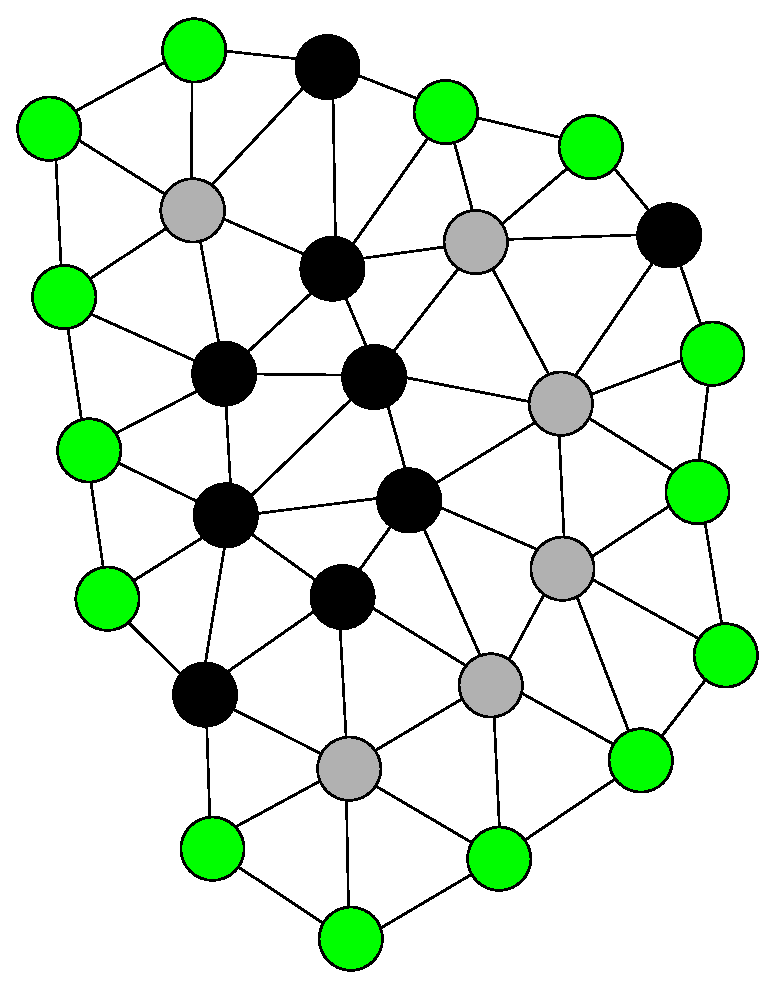
\includegraphics[width=4cm]{CHAPTER-7/figures/PerimeterBotsCircle4}
    \label{fig:InnerPerimeter3}
}
\caption[Inner perimeter effects]{Inner Perimeter Effects}
\label{fig:InnerPerimeterReduction}
\end{figure}

\begin{figure}[H]
\centering
\subfigure[Outer perimeter]{
    \includegraphics[width=4cm]{CHAPTER-7/figures/PerimeterBotsCircle1}
    \label{fig:OuterPerimeter2}
}
\subfigure[Void reduction result]{
    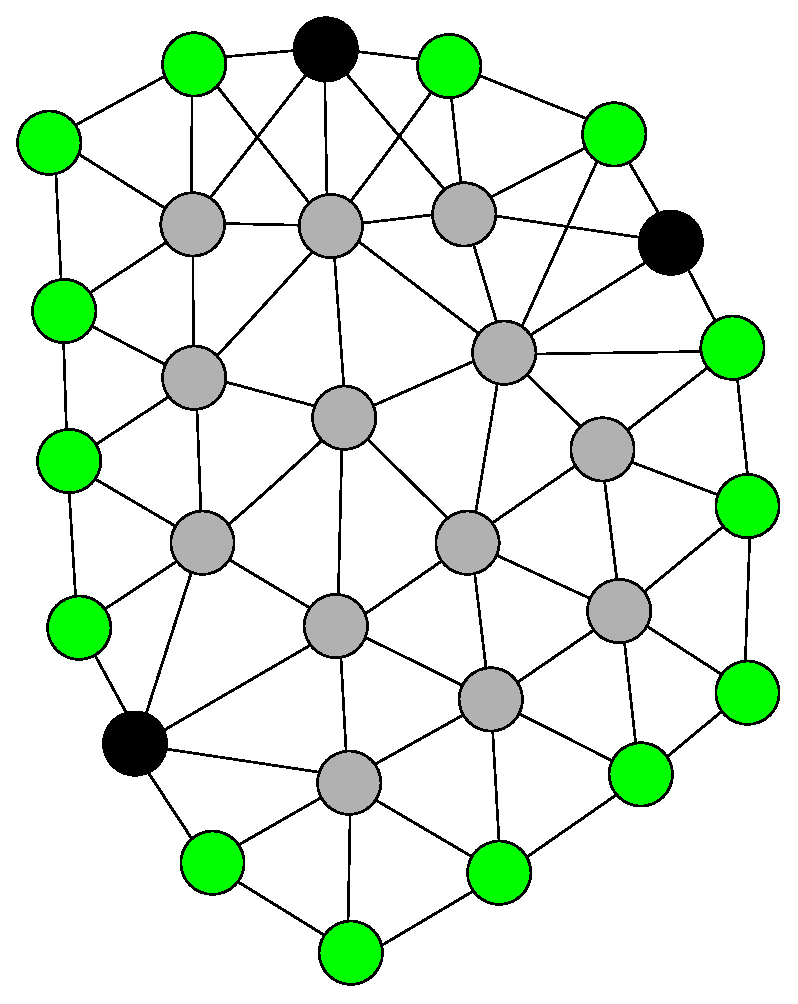
\includegraphics[width=4cm]{CHAPTER-7/figures/PerimeterBotsCircle2}
    \label{fig:OuterPerimeter3}
}
\caption[Outer perimeter effects]{Outer Perimeter Effects}
\label{fig:OuterPerimeterReduction}
\end{figure}

\section{Concave reduction implementation}\label{sec:ConcaveReductionImp}
As previously shown in chapter~\ref{chapter:coordination} detection of a swarm's perimeter can be used to create efficiencies in the use of sensors to coordinate a swarm to a destination. Identifying agents that are suitable for concave reduction to be applied involves the same conditional checks as the perimeter detection algorithm with the addition of a status check on the cyclic-angular-check component~(Section~\ref{reduced:Perimeter2}, page \pageref{reduced:Perimeter2}). In a static swarm, where there are no \textit{destination vectors}, concave reduction will result in a restructuring motion that creates a more `rounded' swarm~(Figure~\ref{fig:OuterPerimeterReduction}). Concave reduction also creates a surround effect as it removes voids from a swarm~(Section~\ref{voids:ObjectSurrounding}). When concave reduction is applied to a mobile swarm the void closing effect can be used to improve reconnaissance coverage as a swarm passes around obstacles~(Figure~\ref{concave:mobileSwarm1}).

Although these effects improve the potential applications of swarms there is a negative impact introduced by concave reduction. When a section of a swarm's perimeter has move concavities than its opposing side concave reduction can create an artificial aggregate \textit{destination vector}. This aggregate vector causes the swarm to move towards the opposing edge. 

To implement void reduction full perimeter detection~(Section~\ref{sec:complexMulti}) is required. Concave reduction does not require the perimeter type to be identified and therefore no communications infrastructure is required~\cite{MD:09,NIM:09,SOM:12,ZFG:13,JG:13}. The main limitation a communications infrastructure imposes on a swarm is the number of agents a swarm can contain. This is due to the propagation time of agent positions throughout the swarm as discussed in~section~\ref{methods:MessagePropogation}~page~\pageref{methods:MessagePropogation}. 

The implementation of concave reduction identification is therefore incorporated into the perimeter detection algorithm~(Algorithm~\ref{algo:checkVisibility}, page \pageref{algo:checkVisibility}). The changes are highlighted in~algorithm~\ref{algo:checkVisibility2}.\\

\begin{algorithm}[H]
\DontPrintSemicolon
\SetAlgoLined
\caption{CheckVisibility}
\KwData{b,angles}
$b.gap \leftarrow \emptyset$\;
$b.concave = False$\;
\For{$i \leftarrow 0$ \KwTo $size(angles)-1$}{
	\eIf{i == size(angles)-1}{
		\If{$cosrule(b,angles[size(angles)-1][0],angles[i][0]$}{
			\If{$angle(b,angles[size(angles)-1][0],angles[i][0]) < 180$}{
				\HiLi$b.concave = True$\;
				\HiLi$b.gap = (angles[size(angles)-1][1],angles[i][1])$\;\tcc{Gap agents (first and last in the dictionary)}
			}		   		   
   		\KwRet{True}
   	}
	}
	{\If{$cosrule(b,angles[i + 1][0],angles[i][0]$}{
			\If{$angle(b,angles[i + 1][0],angles[i][0]) < 180$}{
				\HiLi$b.concave = True$\;
				\HiLi$b.gap = (angles[i + 1][1],angles[i][1])$\;\tcc{Gap agents}
			}		   
			\KwRet{True}
		}
	}
}
\KwRet{False}
\label{algo:checkVisibility2}
\end{algorithm}

The purpose of the changes are to set a status flag to highlight a gap has been detected and to record the agent's neighbour pair that create the concave gap.

\section{Concave reduction agent movement}\label{concave:AgentMovement}
Adding a further characteristic to the motion of a swarm necessitates a revision to the existing agent model as discussed in~section~\ref{methods:BoidModel} page \pageref{methods:BoidModel}. With concave reduction this revision is based upon the identification of the concave perimeter edges as shown in~figure~\ref{concave:VoidConcave1} $(b^{'},b,b^{''})$. 

\begin{figure}[H]
\begin{center}
\includegraphics[width=5cm]{CHAPTER-7/figures/VoidConcave1}
\end{center}
\caption{Agent concave motion\label{concave:VoidConcave1}}
\end{figure}

When an agent is identified as being a component of concave characteristic~(Algorithm~\ref{algo:checkVisibility2}) the normal \textit{movement-direction vector}~(Equation~\ref{eq:BotPhysics1}, page \pageref{eq:BotPhysics1}) is replaced by a \textit{concavity reduction vector}. This new vector causes the agent to move in a direction that will reduce or remove a concave edge by moving the agent towards the identified gap. The effect of this will be to either straighten an outer perimeter or reduce/remove a void. This change in direction increases the distance and magnitude variances (jitter) due to the changes it will induce in the neighbours \textit{interaction vectors}.

Figure~\ref{fig:InterAgentEffects} shows this effect in more detail. Figure~\ref{fig:InterAgentEffect1}~shows the initial positions of the agents before the concave reduction affects the agent. Figure~\ref{fig:InterAgentEffect2}~shows the positive and negative effect on the inter-agent distances that the movement creates. The aggregate change is an increase in the inter-agent distances.

\begin{figure}[H]
\centering
\subfigure[Initial position]{
    \includegraphics[width=5cm]{CHAPTER-7/figures/InterAgentEffect1}
    \label{fig:InterAgentEffect1}
}
\subfigure[Reduced position]{
    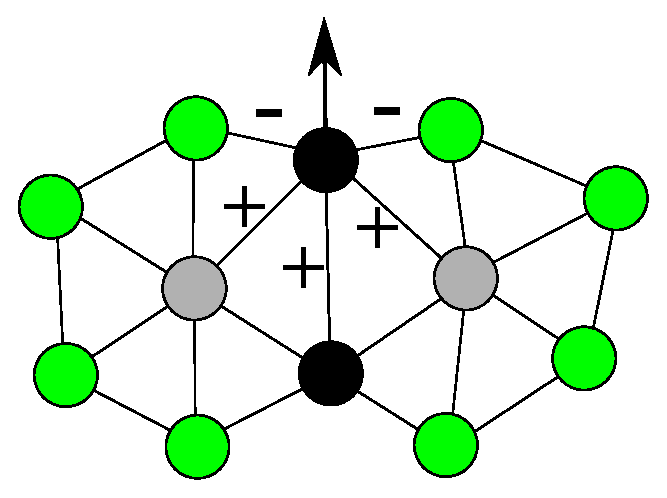
\includegraphics[width=5cm]{CHAPTER-7/figures/InterAgentEffect2}
    \label{fig:InterAgentEffect2}
}
\caption{Inter-agent effects}
\label{fig:InterAgentEffects}
\end{figure}

\subsection{Perimeter Exceptions}\label{concave:Exceptions}
When a swarm is forming or disrupted through either agent failures, catastrophic events or interactions with obstacles sections of the swarm may become isolated. When this occurs the sections can be considered as being a separate sub-swarms. It is also possible for sections of the swarm to remain connected through tenuous links of either 1 or 2 agents as shown in figure~\ref{fig:PerimeterConnectors}. In the case of a link connection~(Figure~\ref{fig:Connector1}) concave reduction can be applied as normal. In the case of a `bridge' link (Figure~\ref{fig:Connector2}) there is an issue in that there is more than one concave gap. As there is no communications infrastructure in swarm models there are limited options for handling this situation. One option is allow the swarming algorithm to apply as usual and no concave reduction takes place; the reasoning being that the overall structure of the swarm is unknown therefore the movement cannot be optimised. An alternative would be to select either the largest or the smallest gap; again as the structure of the swarm is unknown this may not be beneficial. A third option would be to select one of the gaps in some way (randomly, first seen, last seen) and implement the concave reduction at that point. The approach taken in this thesis is to select the first gap that is detected. Selecting the first gap reduces the computational overhead of the algorithm.

\begin{figure}[H]
\centering
\subfigure[Link]{
    \includegraphics[width=4cm]{CHAPTER-7/figures/PerimeterBots4}
    \label{fig:Connector1}
}
\subfigure[Bridge]{
    \includegraphics[width=5cm]{CHAPTER-7/figures/PerimeterBots5}
    \label{fig:Connector2}
}
\caption[Perimeter Connectors]{Perimeter Connectors}
\label{fig:PerimeterConnectors}
\end{figure}

\section{Concave reduction mathematical model}\label{concave:ConcaveVoidReduction1}
Equation~\ref{eq:ConcaveVoidPhysics1} page~\pageref{eq:ConcaveVoidPhysics1} produces a set of agents sorted by angle and algorithm~\ref{algo:checkVisibility2} page~\pageref{algo:checkVisibility2} produces a set ($b.gap \equiv G_b$) consisting of the first two agents identified as creating a `gap' in agent $b$'s neighbours. Equation~\ref{eq:ConcaveVoidPhysics3} calculates the centroid of the gap agents. 

\begin{center}
\begin{equation}‎
\label{eq:ConcaveVoidPhysics3}
D_{pos}(b) =‎ \frac{1}{2}\mathlarger{\sum_{b' \in G_b}}{b'} 
\end{equation}‎
\end{center}

The centroid $D_{pos}(b)$ is then used to calculate the \textit{concavity reduction vector}~(Equation~\ref{eq:ConcaveVoidPhysics3a}).

\begin{center}
\begin{equation}‎
\label{eq:ConcaveVoidPhysics3a}
D(b) =‎ D_{pos}b 
\end{equation}‎
\end{center}

$D(b)$~is a vector derived from the identified centroid of the neighbour gap~($G_b$) to the parent agent~($b$). This new vector is the \textit{concavity vector} used to implement the concave reduction movement~(Equation~\ref{eq:ConcaveVoidPhysics3a}).

This derived movement is specifically for reducing the anomaly of which the agent is a part. The concave reduction movement needs to be enhanced to take into consideration an agent's surroundings. Due to proximity it can be assumed that there are no agents in the path between the agent and the gap, however there may be an obstacle. The \textit{concavity vector} must include an obstacle avoidance component~(Equation~\ref{eq:ConcaveVoidPhysics4}) as shown in~section~\ref{section:ObstacleSection} on page \pageref{section:ObstacleSection}. As with all the previous vector based calculations a weighting is applied to the calculated \textit{concavity vector}~$k_{cr}$ to allow the model to vary the intensity of the effect. The resultant vector is then normalised to produce the \textit{concavity reduction vector} as shown in~equation~\ref{eq:ConcaveVoidPhysics4}. 

\begin{center}
\begin{equation}‎
\label{eq:ConcaveVoidPhysics4}
V(b) = (k_{cr}D(b) + k_ov_o(b))\string^
\end{equation}‎
\end{center}

\section{Application of concave reduction on perimeter agents}
If there is a `gap' on a perimeter then the \textit{concavity reduction vector} is applied instead of the normal \textit{interaction vector}. To test this effect a baseline is established for a comparison.

Using the same swarm deployment as used in chapter~\ref{chapter:metric} a baseline simulation is used as a comparison to identify the changes created by the introduction of the \textit{concavity reduction vectors}. The comparison takes into consideration not just the jitter identified by the distance and magnitude metrics but also the effect on the number of perimeter agents. The main effect concave reduction on a swarm's structure is to reduce the size of the perimeter. Table~\ref{tab:BaselineConcaveReduction} shows the simulation parameters for both the baseline and the concave reduction experiments.

\begin{table}[H]
\begin{center}
\begin{tabular}{| p{2.3cm} | p{2cm} | p{2cm} | p{5cm} |}
\hline
\bf Weight \bf component & \bf Baseline \bf swarm & \bf Concave \bf reduction & \bf Description \\ \hline
Sample rate & 100 & 100 & ms - Unit sampling interval\\  \hline
$k_{cr}$ & 0 & 100 & weight adjuster for concavity reduction vector\\  \hline
$k_c$ & 5 & 5 & weight adjuster for cohesion field\\  \hline
$k_r$ & 15 & 15 & weight adjuster for repulsion field\\  \hline
$k_d$ & 0 & 0 & weight adjuster for destination vector 0 for static baseline 100 from directional\\  \hline
Repulsion Boundary & 70 & 70 & units\\  \hline
Neighbour Distance & 80 & 80 & units\\  \hline
Speed & 20 & 20 & units/s\\  \hline
\end{tabular}\caption{Baseline comparison for concave reduction} \label{tab:BaselineConcaveReduction}
\end{center}
\end{table}

Figure~\ref{concave:BaselineConcaveEffectDist} shows the changes in the inter-agent distances that result from the concave reduction. The experiment demonstrates that with concave reduction the average distance increases and the variance of the distances increases. This is due to the `pulling' effect of the \textit{concavity reduction vector} on the perimeter. The algorithm distorts the distribution of the agents as discussed in~section~\ref{concave:AgentMovement}. The initial expansion of the swarm is similar for the baseline and the concave reduction however at 9 seconds into the simulation the \textit{concavity reduction vectors} affects the swarm sufficiently to prevent the average distance reducing to the same level as the baseline. Once the swarm has stabilised with the concave reduction enabled the average distance and variance remain constant but above the baseline.

%BASELINE-CONCAVE-DIST.py
\begin{figure}[H]
\begin{center}
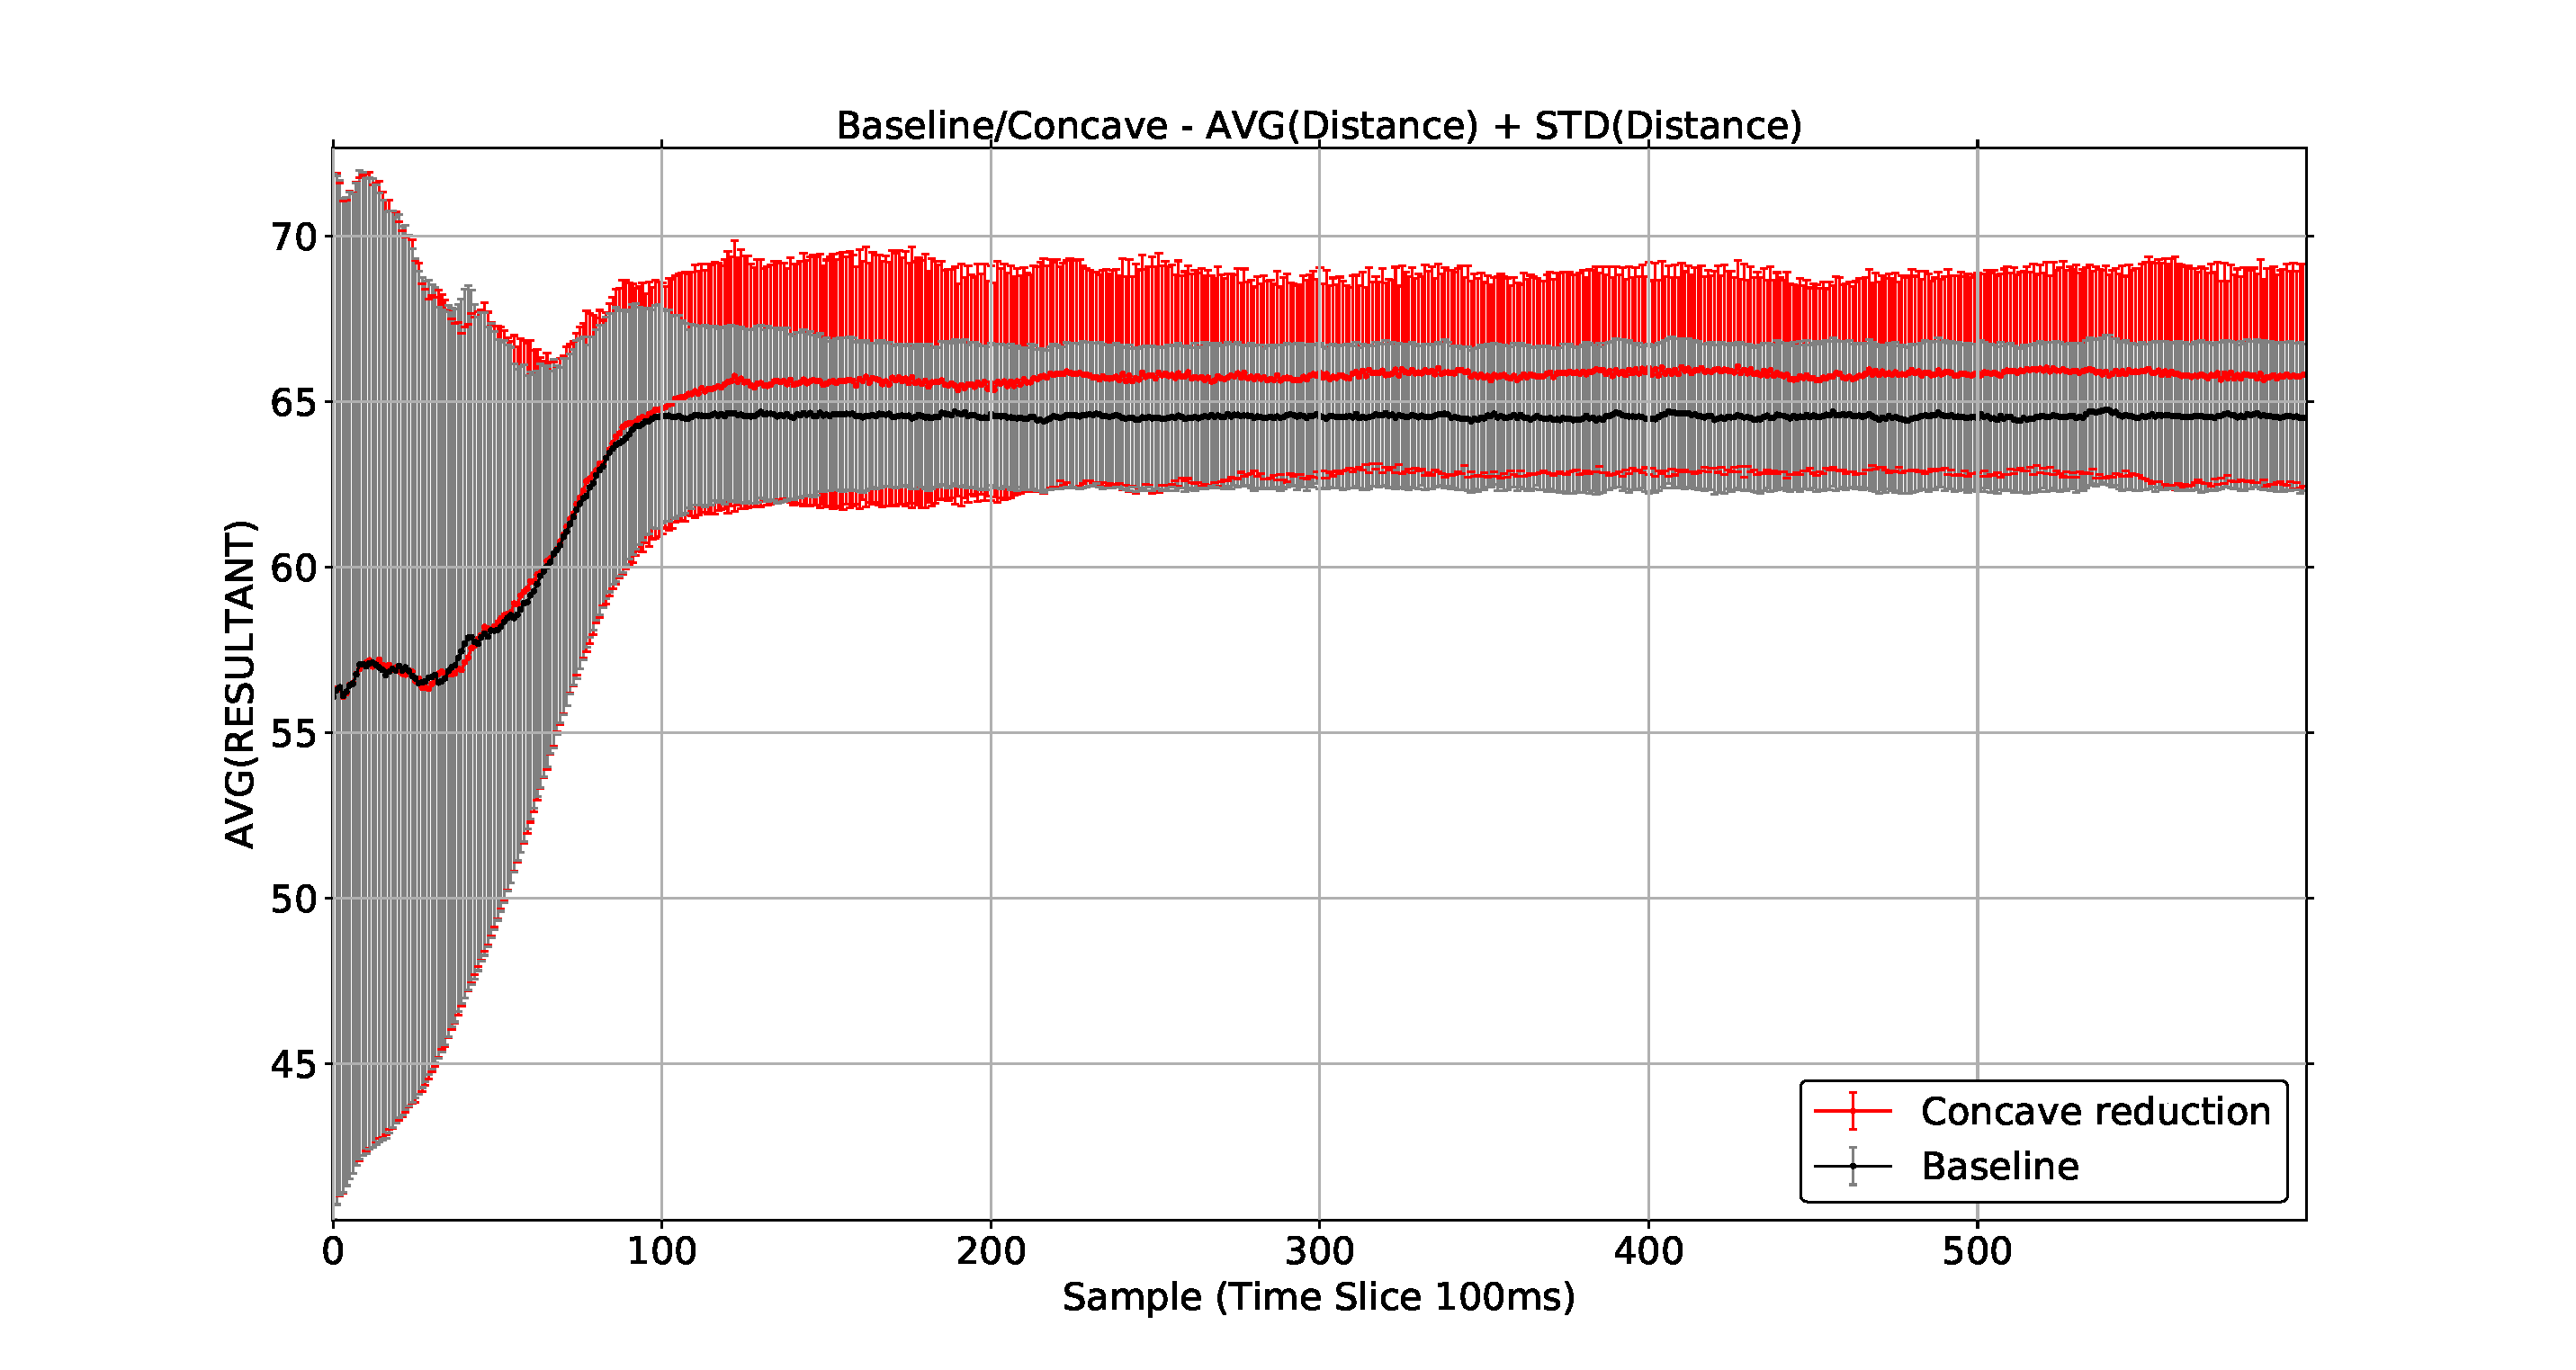
\includegraphics[width=14cm]{CHAPTER-7/figures/BaselineConcaveEffectDist}
\end{center}
\caption{Baseline/Concave effect distance \label{concave:BaselineConcaveEffectDist}}
\end{figure}

Figure~\ref{concave:BaselineConcaveEffectMag} shows the change in the \textit{inter-agent vector magnitudes} that the concave reduction introduces. Both the average magnitude increases and the variance. The magnitude increases as the \textit{concavity reduction vector} has caused the agents to move outwards increasing the area of the swarm. The increase in cohesion is a direct result of the increased distance. The field effects still intersect but due to the average distance of the agents being further apart the repulsion is reduced. The agents being further apart causes the increase in cohesion as the algorithm attempts to prevents the swarm from breaking up. The variance increase is caused by the concave reduction effect moving selected agents into less optimal positions.

The \textit{inter-agent vector magnitude} calculations in these experiments are based on the positions of the agents and the cohesion and repulsion field effects. The \textit{concavity reduction vector} is not part of the metric calculation. The \textit{concavity reduction vector} is only applied to an agent for movement calculation. 

%BASELINE-CONCAVE-MAG.py
\begin{figure}[H]
\begin{center}
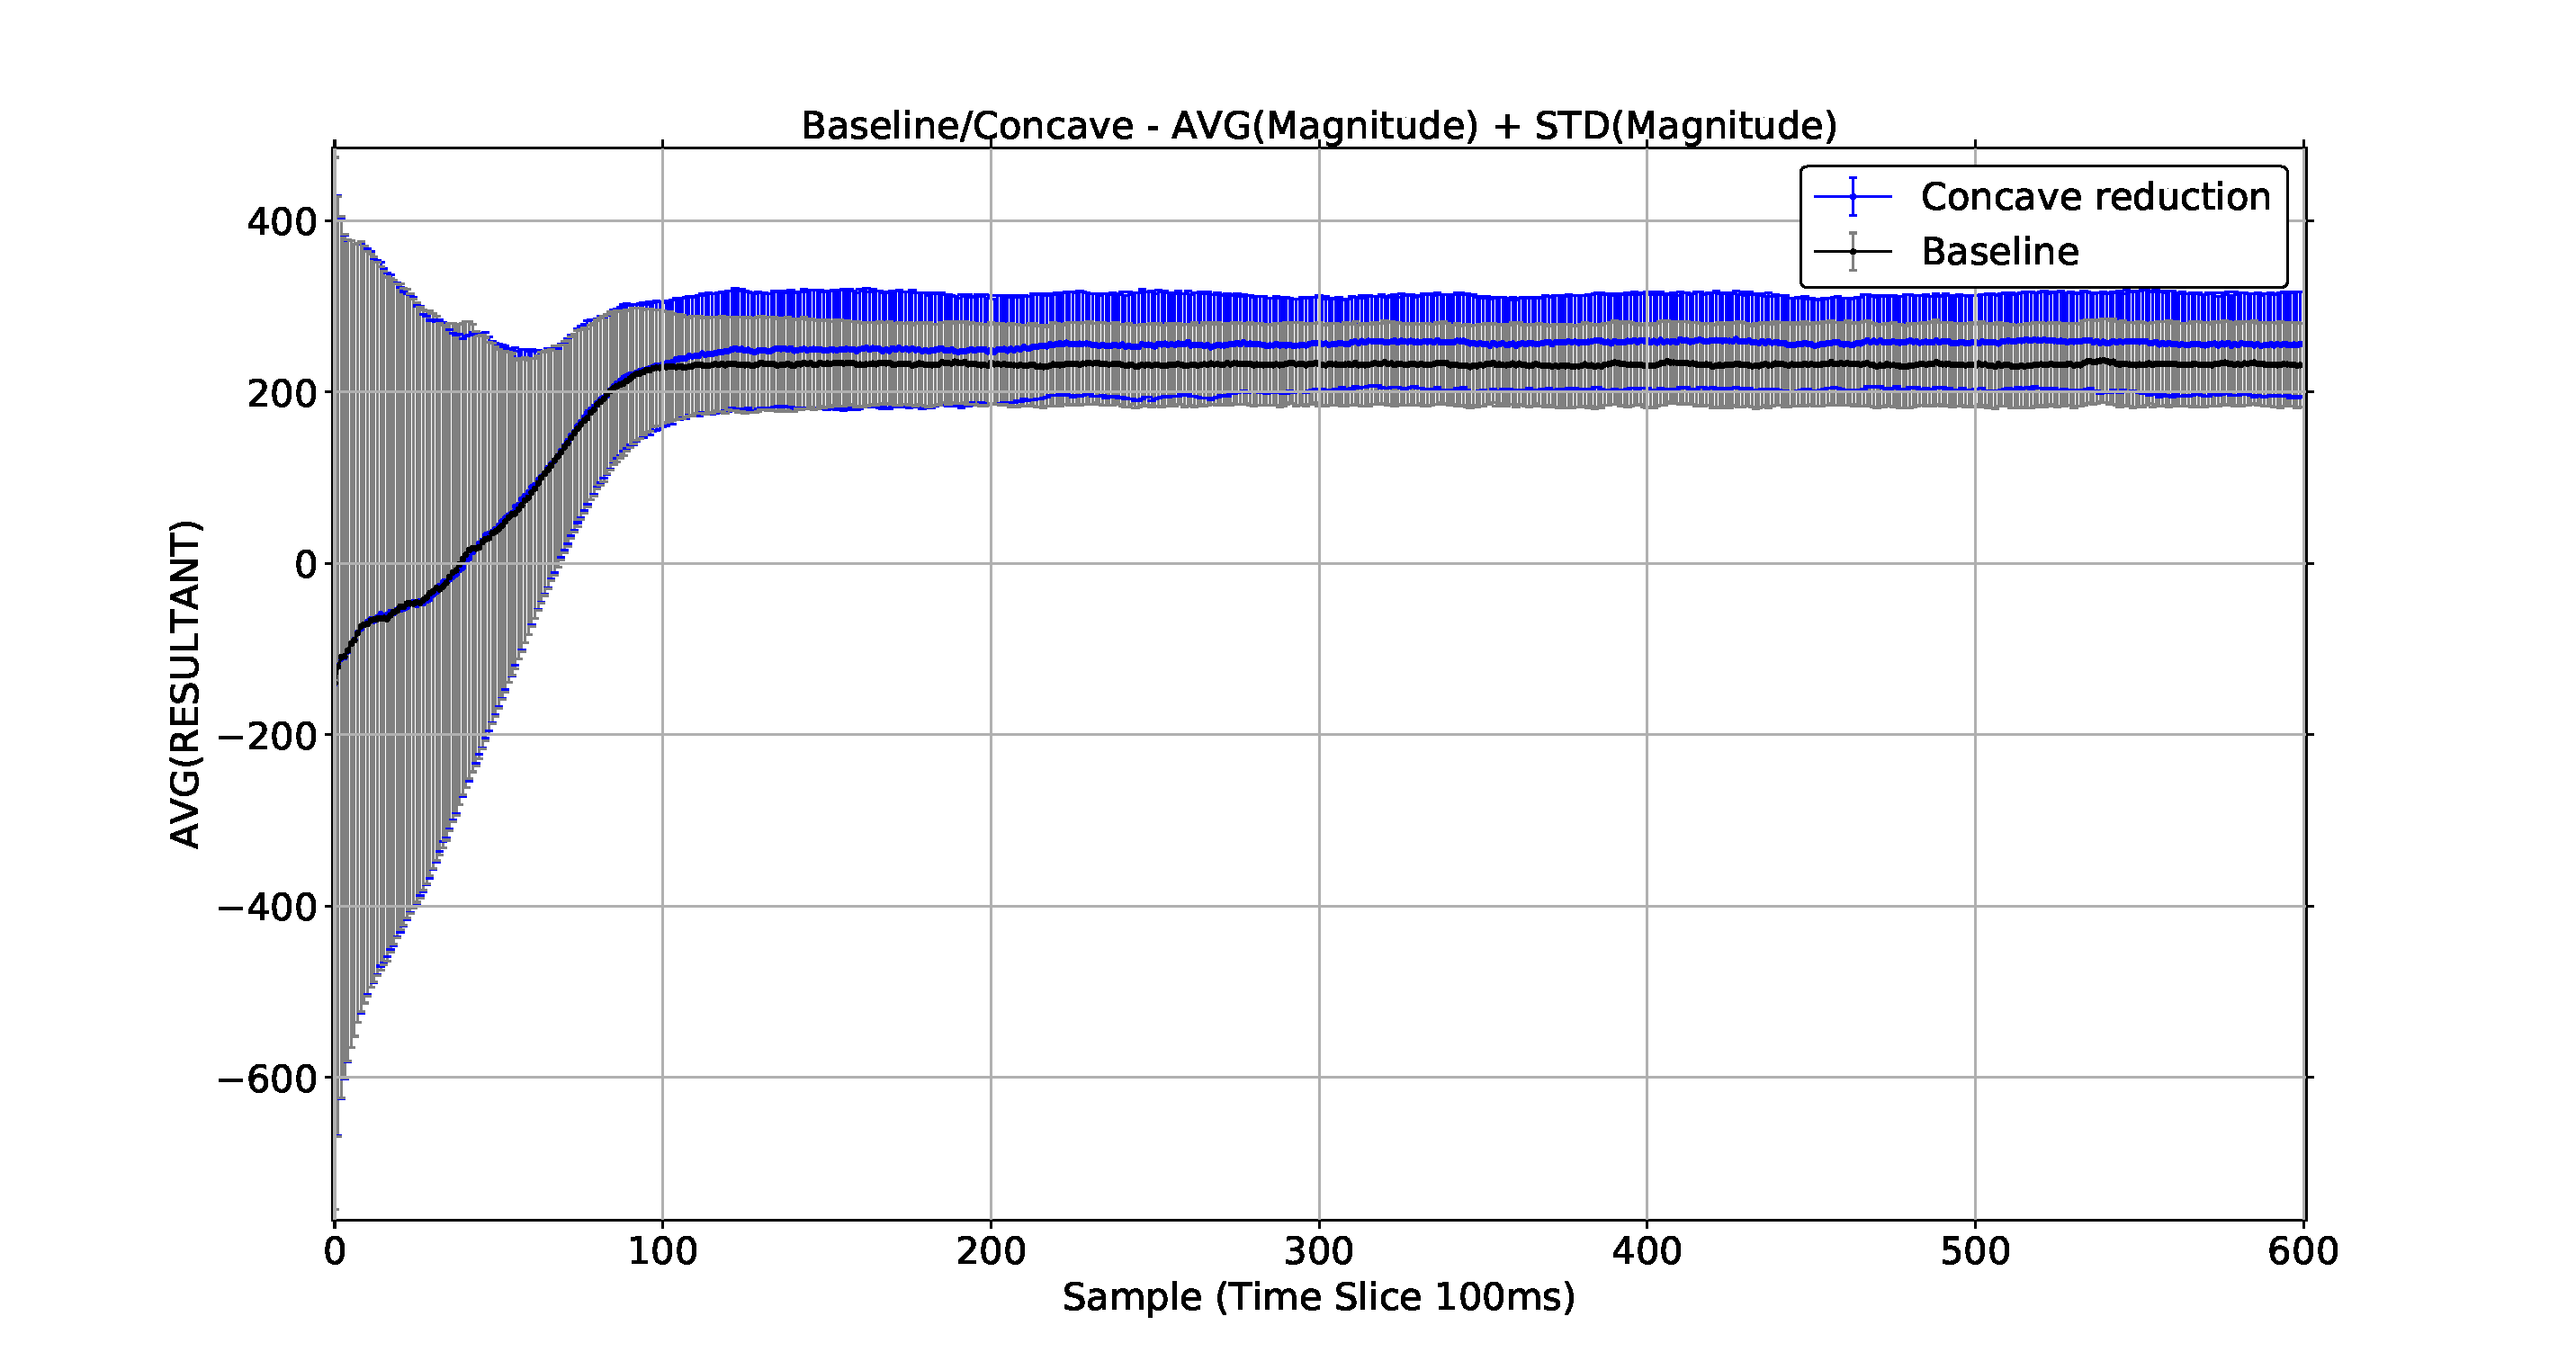
\includegraphics[width=14cm]{CHAPTER-7/figures/BaselineConcaveEffectMag}
\end{center}
\caption{Baseline/Concave effect magnitude\label{concave:BaselineConcaveEffectMag}}
\end{figure}

Figure~\ref{concave:BaselineConcavePerimeter} shows the effect on the number of perimeter agents. Initially the perimeter size is minimally affected due to the swarm's compression however after the expansion phase of the swarm (8 seconds) more perimeter agents are identified as concave edges are formed. As these concave edges are `straightened' they create further anomalies that ripple through the swarm. This rippling is identified by the erratic changes in the number of perimeter agents. After approximately 30 seconds the swarm has been forced into a less angular structure with curved edges and the number of perimeter agents falls below the minimum of the baseline. The shape of the swarm is still undergoing change following this and the perimeter count continues to fluctuate.
%PERIMETER8070CONCAVE.py
\begin{figure}[H]
\begin{center}
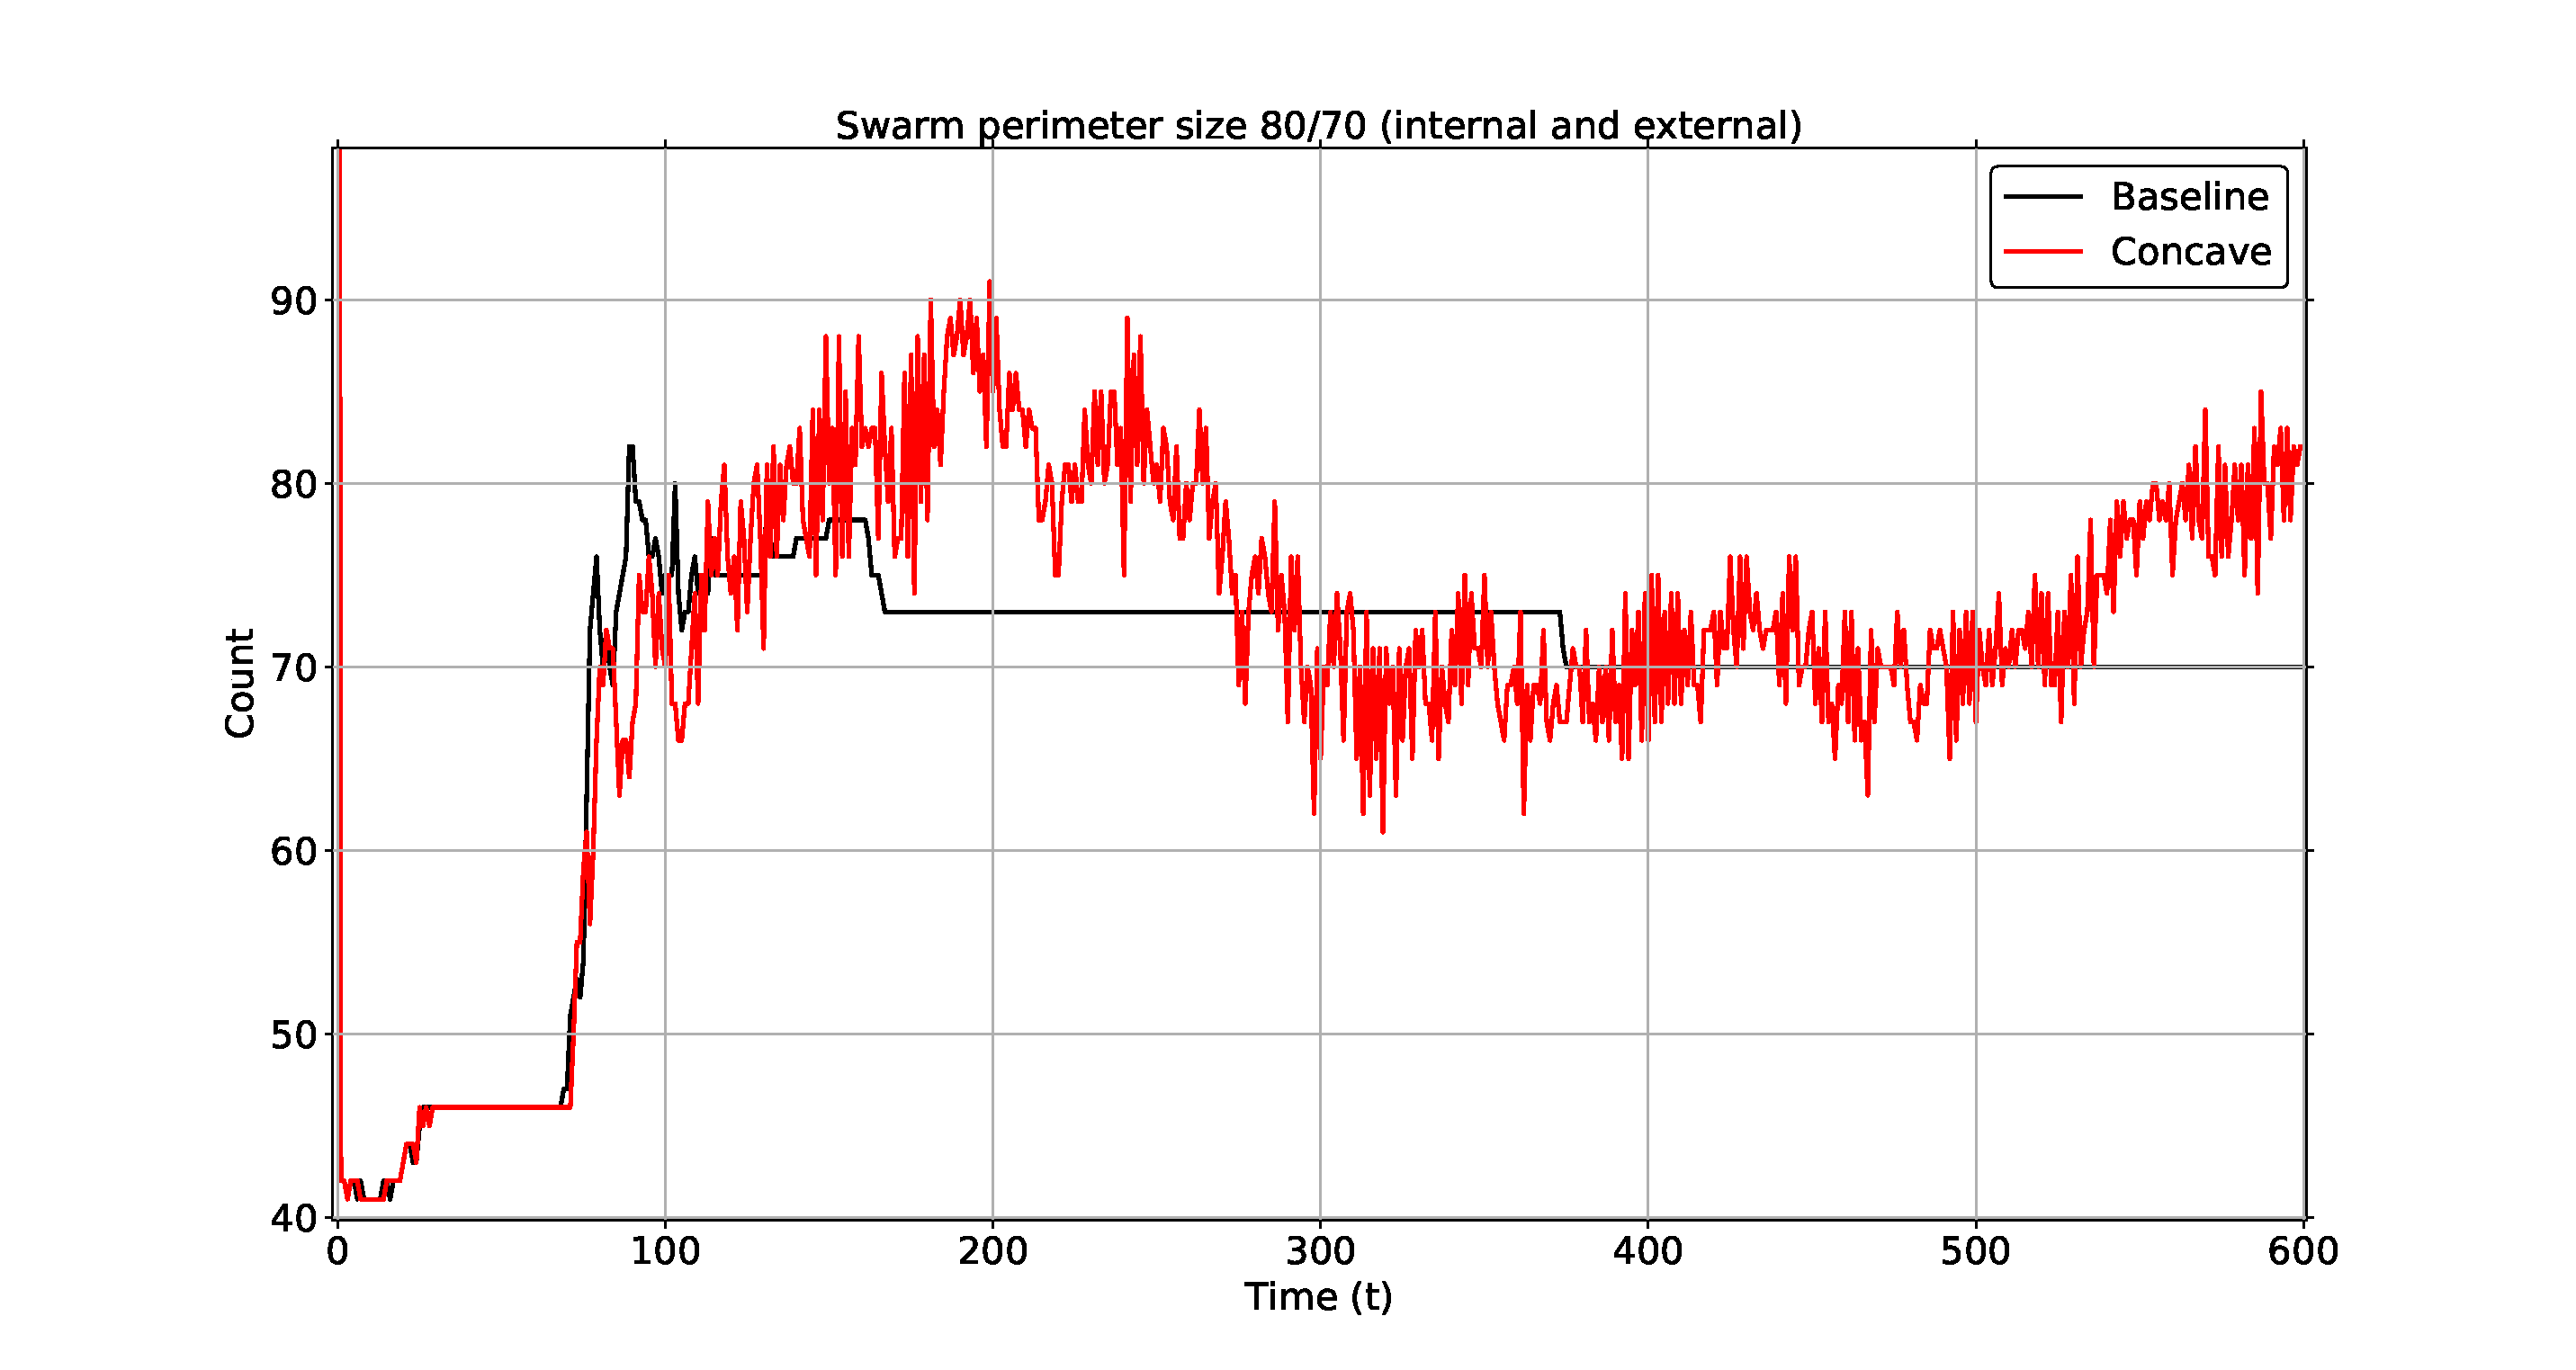
\includegraphics[width=14cm]{CHAPTER-7/figures/BaselineConcavePerimeter}
\end{center}
\caption{Baseline/Concave perimeter size\label{concave:BaselineConcavePerimeter}}
\end{figure}

The effect on the structure of the swarm caused by the concave perimeter agents moving towards the gap agents is to pull the internal agents forward. This pulling causes the swarm to develop a more rounded structure but the effect also have a negative impact. If the tolerance of the agent's movements (the difference between the agent ranges for repulsion and cohesion) is too small then the distortion effect of the concave reduction can create additional voids. The perimeter agents will then move so as to remove the defect~(Figure~\ref{fig:OuterPerimeterJitter1}). Following the void creation the agents are now impacted by a second concave reduction from the newly created void and the anomaly on the perimeter edge `snaps' back closing the void~(Figure~\ref{fig:OuterPerimeterJitter2}). This process repeats itself creating an instability in the number of perimeter agents which is highlighted in~figure~\ref{concave:BaselineConcavePerimeter} as the erratic change in the number of agents. 

\begin{figure}[H]
\centering
\subfigure[Snapping effect closed]{
    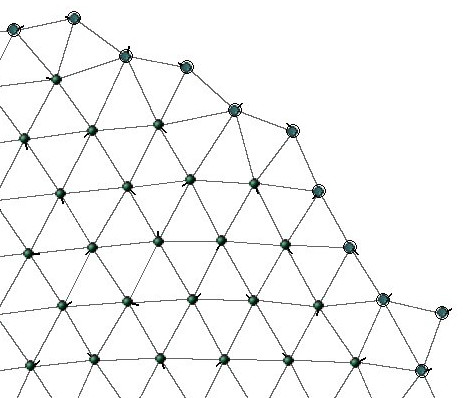
\includegraphics[width=5cm]{CHAPTER-7/figures/OuterPerimeterJitter1}
    \label{fig:OuterPerimeterJitter1}
}
\subfigure[Snapping effect open]{
    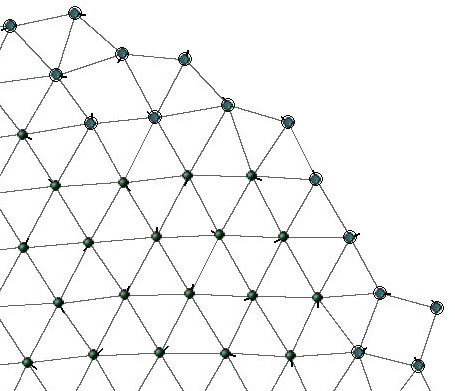
\includegraphics[width=5cm]{CHAPTER-7/figures/OuterPerimeterJitter2}
    \label{fig:OuterPerimeterJitter2}
}
\caption{Outer perimeter snapping effects}
\label{fig:InducedJitter}
\end{figure}

Figure~\ref{concave:BaselineConcaveEffectPath1} shows the paths of the agents in the swarm with concave reduction (red) and the baseline (black). The paths of the agents are initially very similar as the swarm expands but as the \textit{interaction vector magnitudes} rise and the swarm stabilises the effect of the \textit{concavity reduction vectors} start to noticeably influence the swarm structure. The most noticeable effect is on the perimeter where the agents have expanded then instead of stabalising to relatively stable fixed position there is drifting effect occurring due to the imbalance of the initial deployment structure (more anomalies on one side). The swarm also becomes more `rounded' in appearance. 

%COVERBASELINE1.py
\begin{figure}[H]
\begin{center}
\includegraphics[width=14cm]{CHAPTER-7/figures/BaselineConcaveEffectPath1}
\end{center}
\caption{Baseline/Concave path effect (after 600 iterations / 60s)\label{concave:BaselineConcaveEffectPath1}}
\end{figure}

Figure~\ref{concave:BaselineConcaveEffectPath2} shows a more detailed view of the structure within the swarm. The baseline (black) paths show the swarm expanding and then settling to a hexagonal pattern which appears to oscillate slightly (jitter) when the swarm has reached its optimum distribution. The concave reduction swarm agents paths (red) show the swarm expanding in a similar way but once fully expanded the concave reduction causes the swarm to move with a slight directional bias.

%COVERBASELINE1.py
\begin{figure}[H]
\begin{center}
\includegraphics[width=14cm]{CHAPTER-7/figures/BaselineConcaveEffectPath2}
\end{center}
\caption{Baseline/Concave path effect (after 600 iterations / 60s)\label{concave:BaselineConcaveEffectPath2}}
\end{figure}

To reduce the `snapping' effect (Figure~\ref{fig:InducedJitter}), the field effect parameters can be adjusted to create a greater tolerance in the agent interactions. This can be achieved by either reducing the agents repulsion field and maintaining the neighbour field effect or increasing the neighbour field effect and maintaining the repulsion field effect. These changes affect the structure of the swarm but ensure that the agents to stay within the cohesion field when moving to implement the concave reduction the agents are therefore `held' by the cohesion field effect preventing the `snap'. These changes in the field effect can be shown experimentally using the parameters in~table~\ref{tab:BaselineConcaveReduction2}. 

\begin{table}[H]
\begin{center}
\begin{tabular}{| p{2.3cm} | p{2cm} | p{2cm} | p{5cm} |}
\hline
\bf Weight \bf component & \bf Baseline \bf swarm & \bf Concave \bf reduction & \bf Description \\ \hline
Sample rate & 100 & 100 & ms - Unit sampling interval\\  \hline
$k_{cr}$ & 0 & 100 & weight adjuster for concavity reduction vector\\  \hline
$k_c$ & 5 & 5 & weight adjuster for cohesion field\\  \hline
$k_r$ & 15 & 15 & weight adjuster for repulsion field\\  \hline
$k_d$ & 0 & 0 & weight adjuster for destination vector 0 for static baseline 100 from directional\\  \hline
Repulsion Boundary & 60 & 60 & units\\  \hline
Neighbour Distance & 80 & 80 & units\\  \hline
Speed & 20 & 20 & units/s\\  \hline
\end{tabular}\caption{Baseline comparison for concave reduction} \label{tab:BaselineConcaveReduction2}
\end{center}
\end{table}

Figure~\ref{concave:BaselineConcaveEffectDist8060} shows a comparison of the agent movements based on distance for the revised field effects. The graph shows that the swarm settles to a distance that is closer due to the reduced repulsion field. The graph also shows that the concave reduction still induces additional jitter as the variance is still greater than the baseline but due to the reduced snapping the perimeter agent count shows greater stability~(Figure~\ref{concave:BaselineConcavePerimeter8060}). 
%BASELINE-COMPRESS-DIST-8060.py
\begin{figure}[H]
\begin{center}
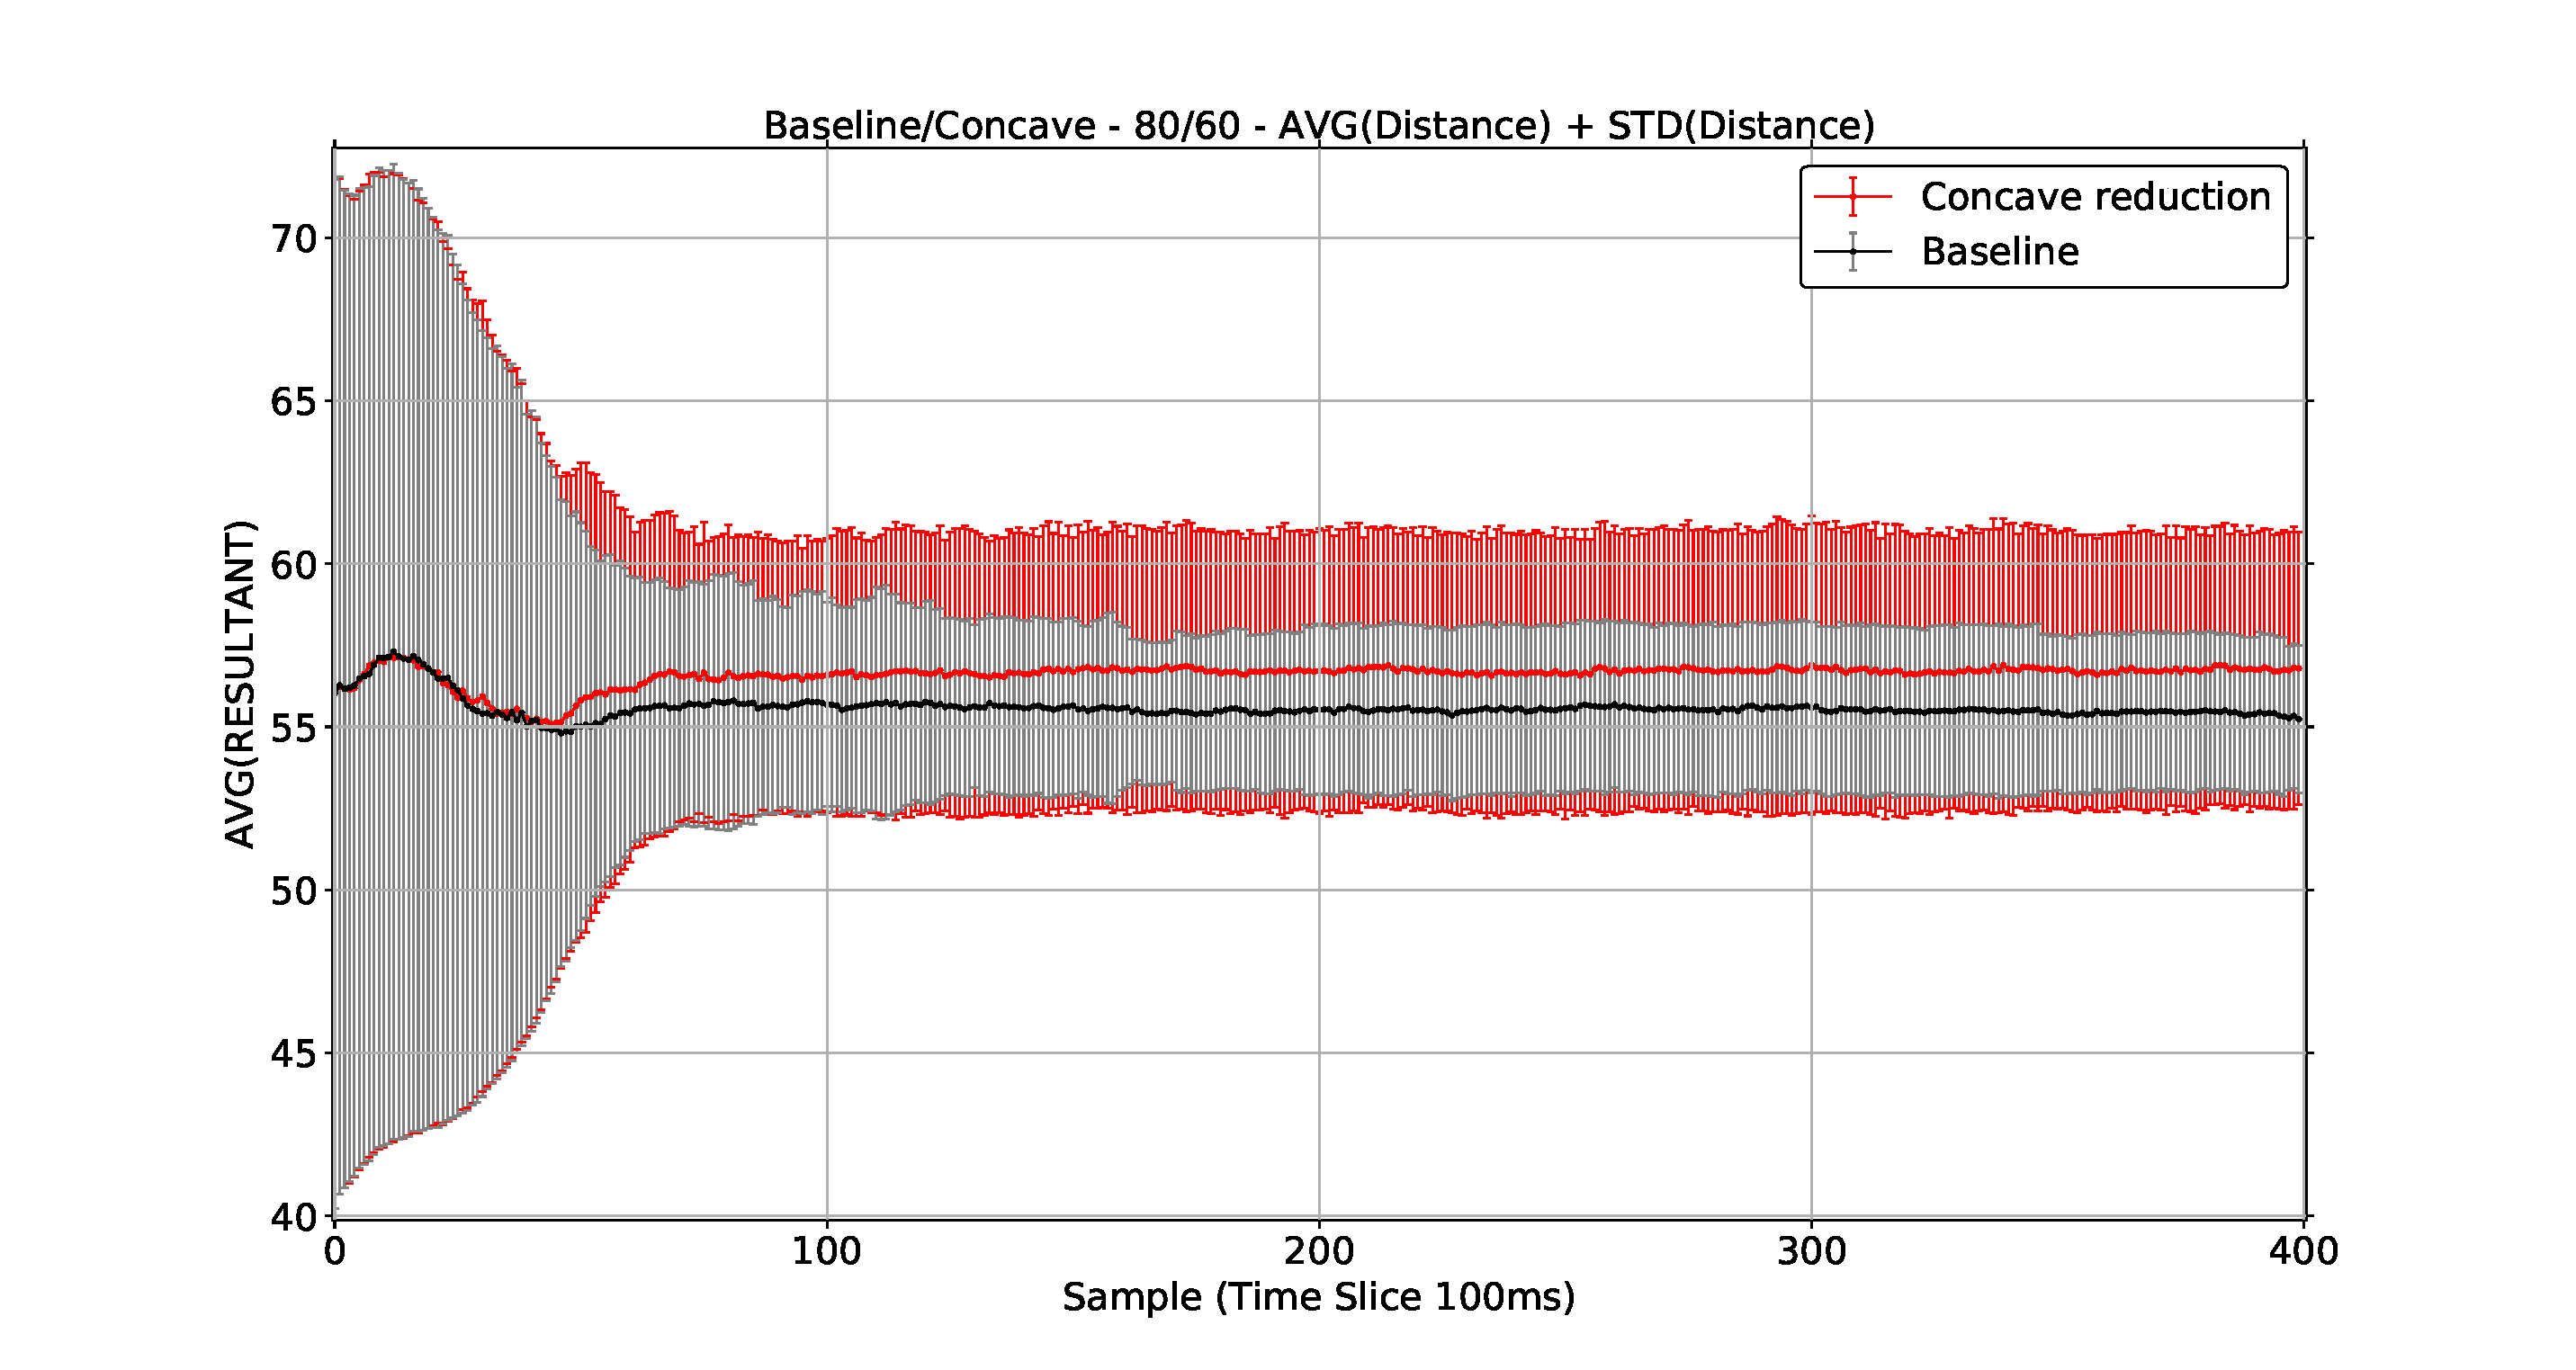
\includegraphics[width=14cm]{CHAPTER-7/figures/BaselineConcaveEffectDist8060}
\end{center}
\caption{Baseline/Concave effect distance (cohesion filed 80/ repulsion field 60)\label{concave:BaselineConcaveEffectDist8060}}
\end{figure}

Figure~\ref{concave:BaselineConcaveEffectMag8060} shows that the \textit{inter-agent vector magnitude} is reduced due to the reduced cohesion from the agent proximity and the \textit{concavity reduction vector magnitude} impact is reduced due to less anomalies occurring on the perimeter.
%BASELINE-COMPRESS-MAG-8060.py
\begin{figure}[H]
\begin{center}
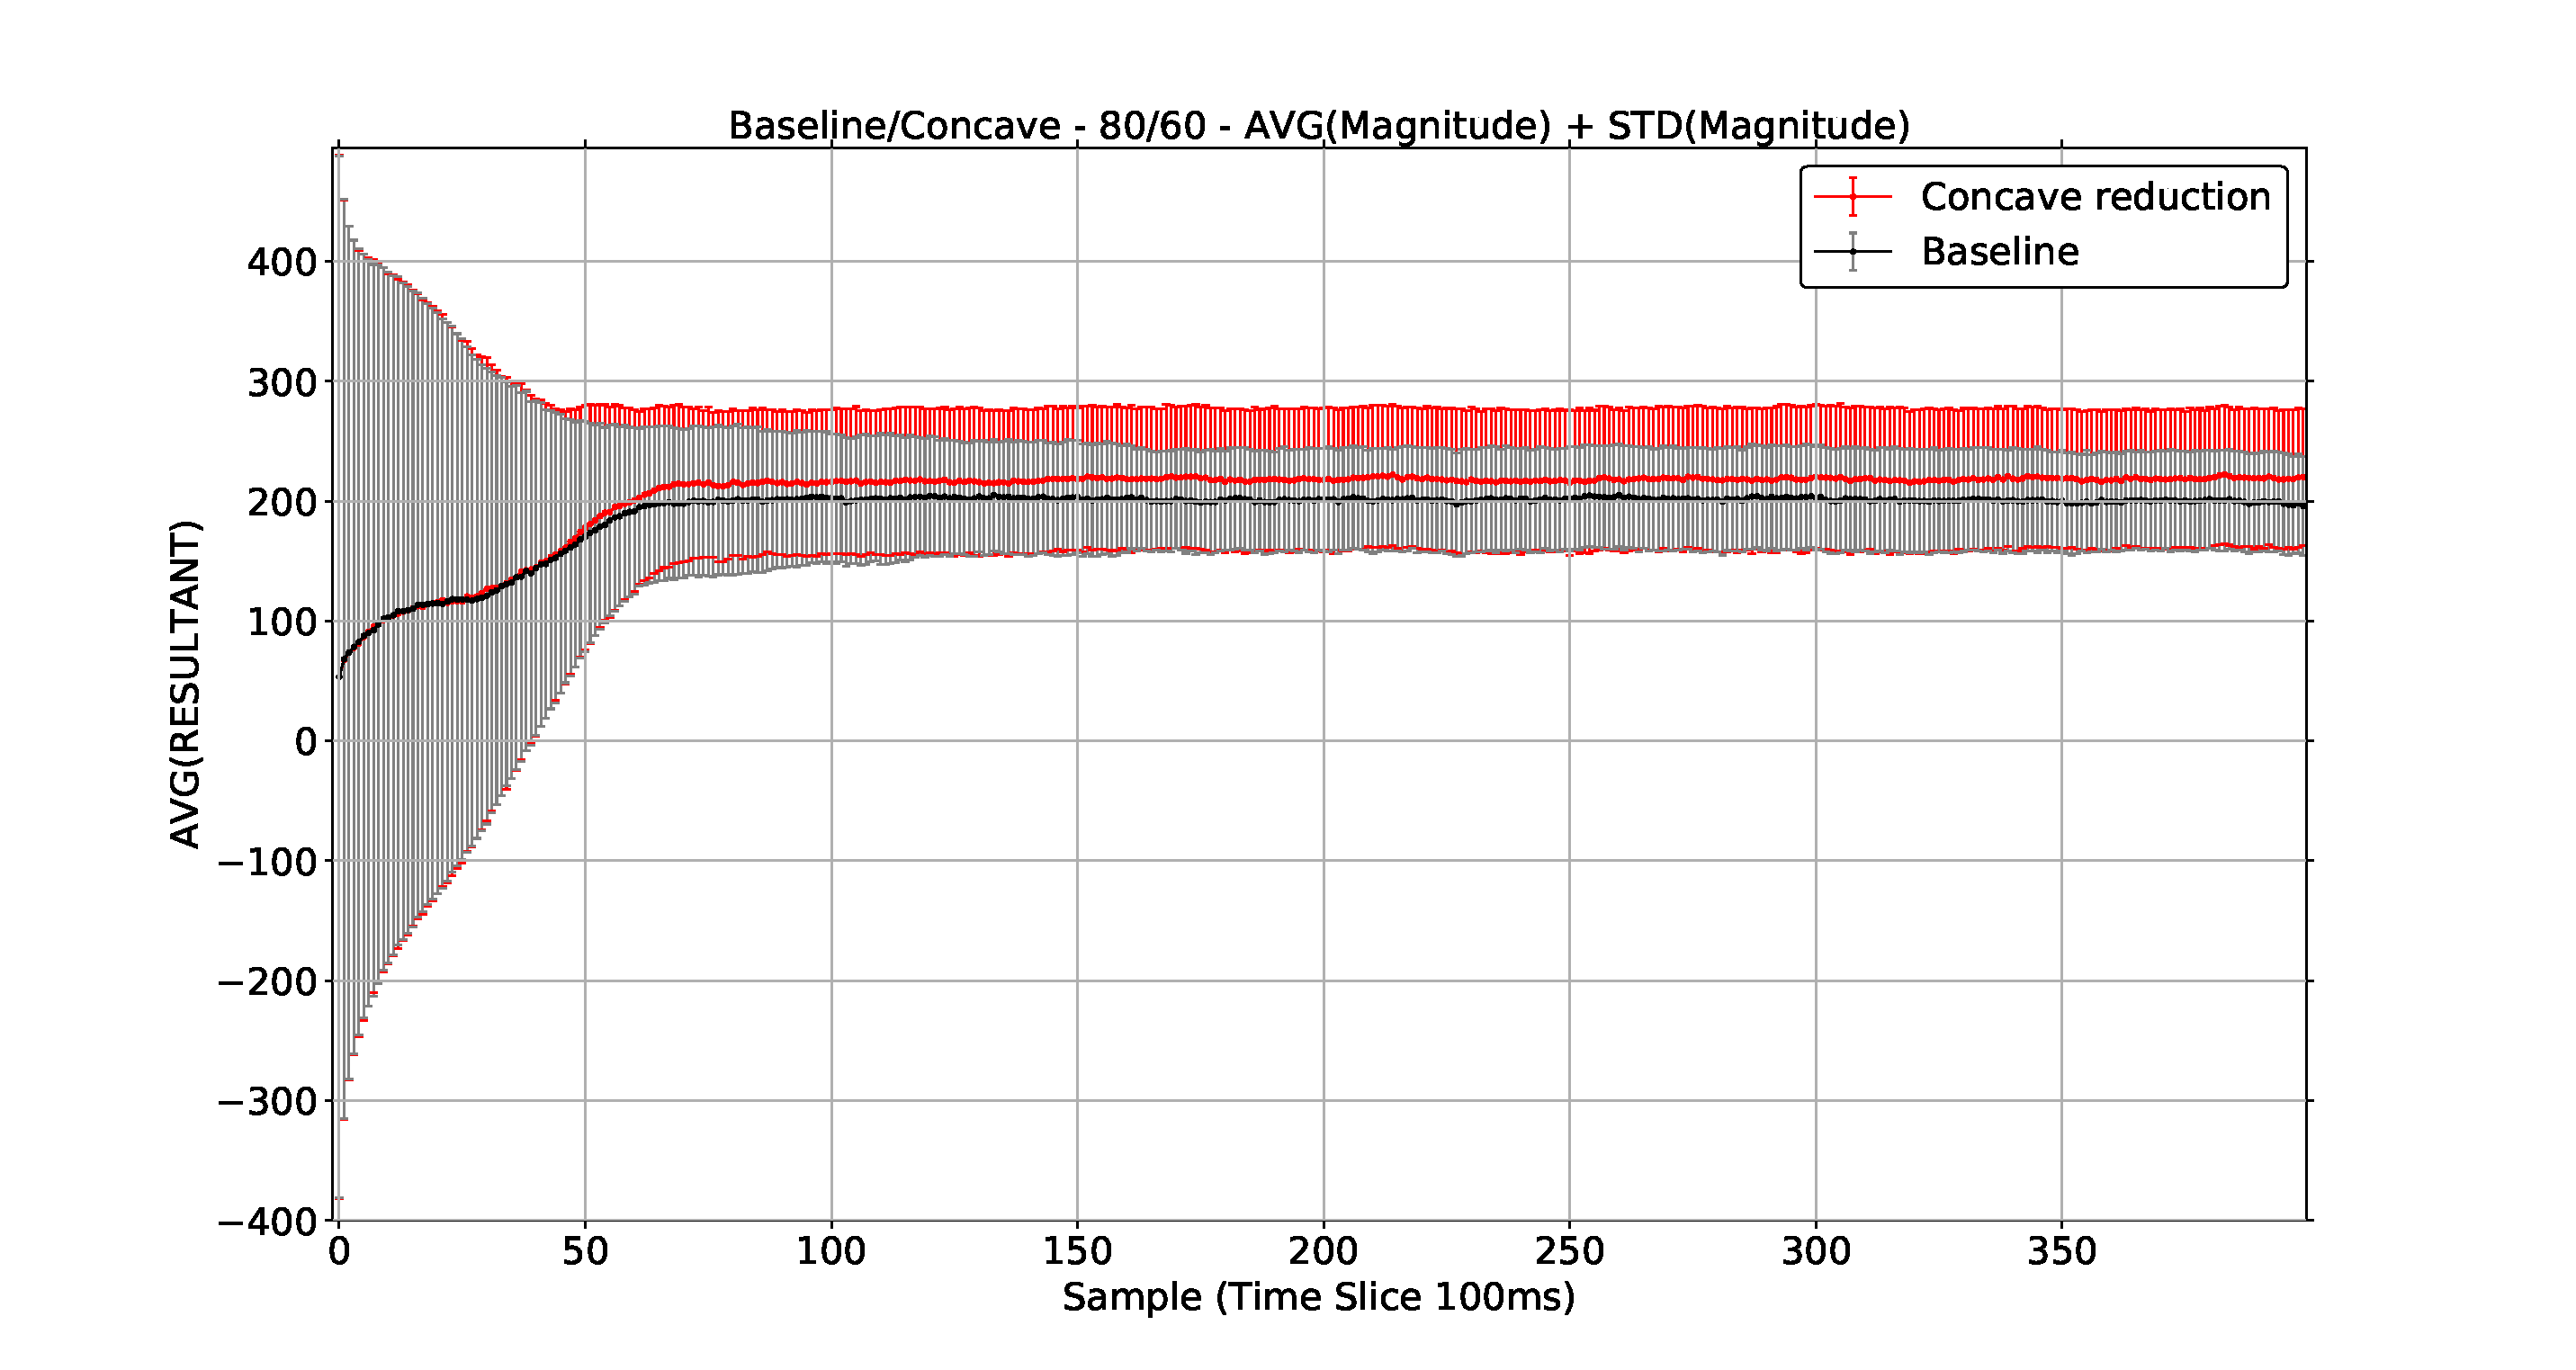
\includegraphics[width=14cm]{CHAPTER-7/figures/BaselineConcaveEffectMag8060}
\end{center}
\caption{Baseline/Concave effect magnitude (cohesion field 80 / repulsion field 60)\label{concave:BaselineConcaveEffectMag8060}}
\end{figure}

Figure~\ref{concave:BaselineConcavePerimeter8060} shows the changes in the perimeter size from the baseline and the concave reduction swarms. The concave reduction still creates an erratic perimeter count but the variation is reduced. On aggregate for the run the concave reduction has reduced the perimeter size. The revised effects also reduce the snapping effect and the swarm has an improved structure. The concave reduction creates a perimeter which fluctuates between 45-50 agents where as the baseline swarm settles to 49 agents.
 
%PERIMETER8060CONCAVE.py
\begin{figure}[H]
\begin{center}
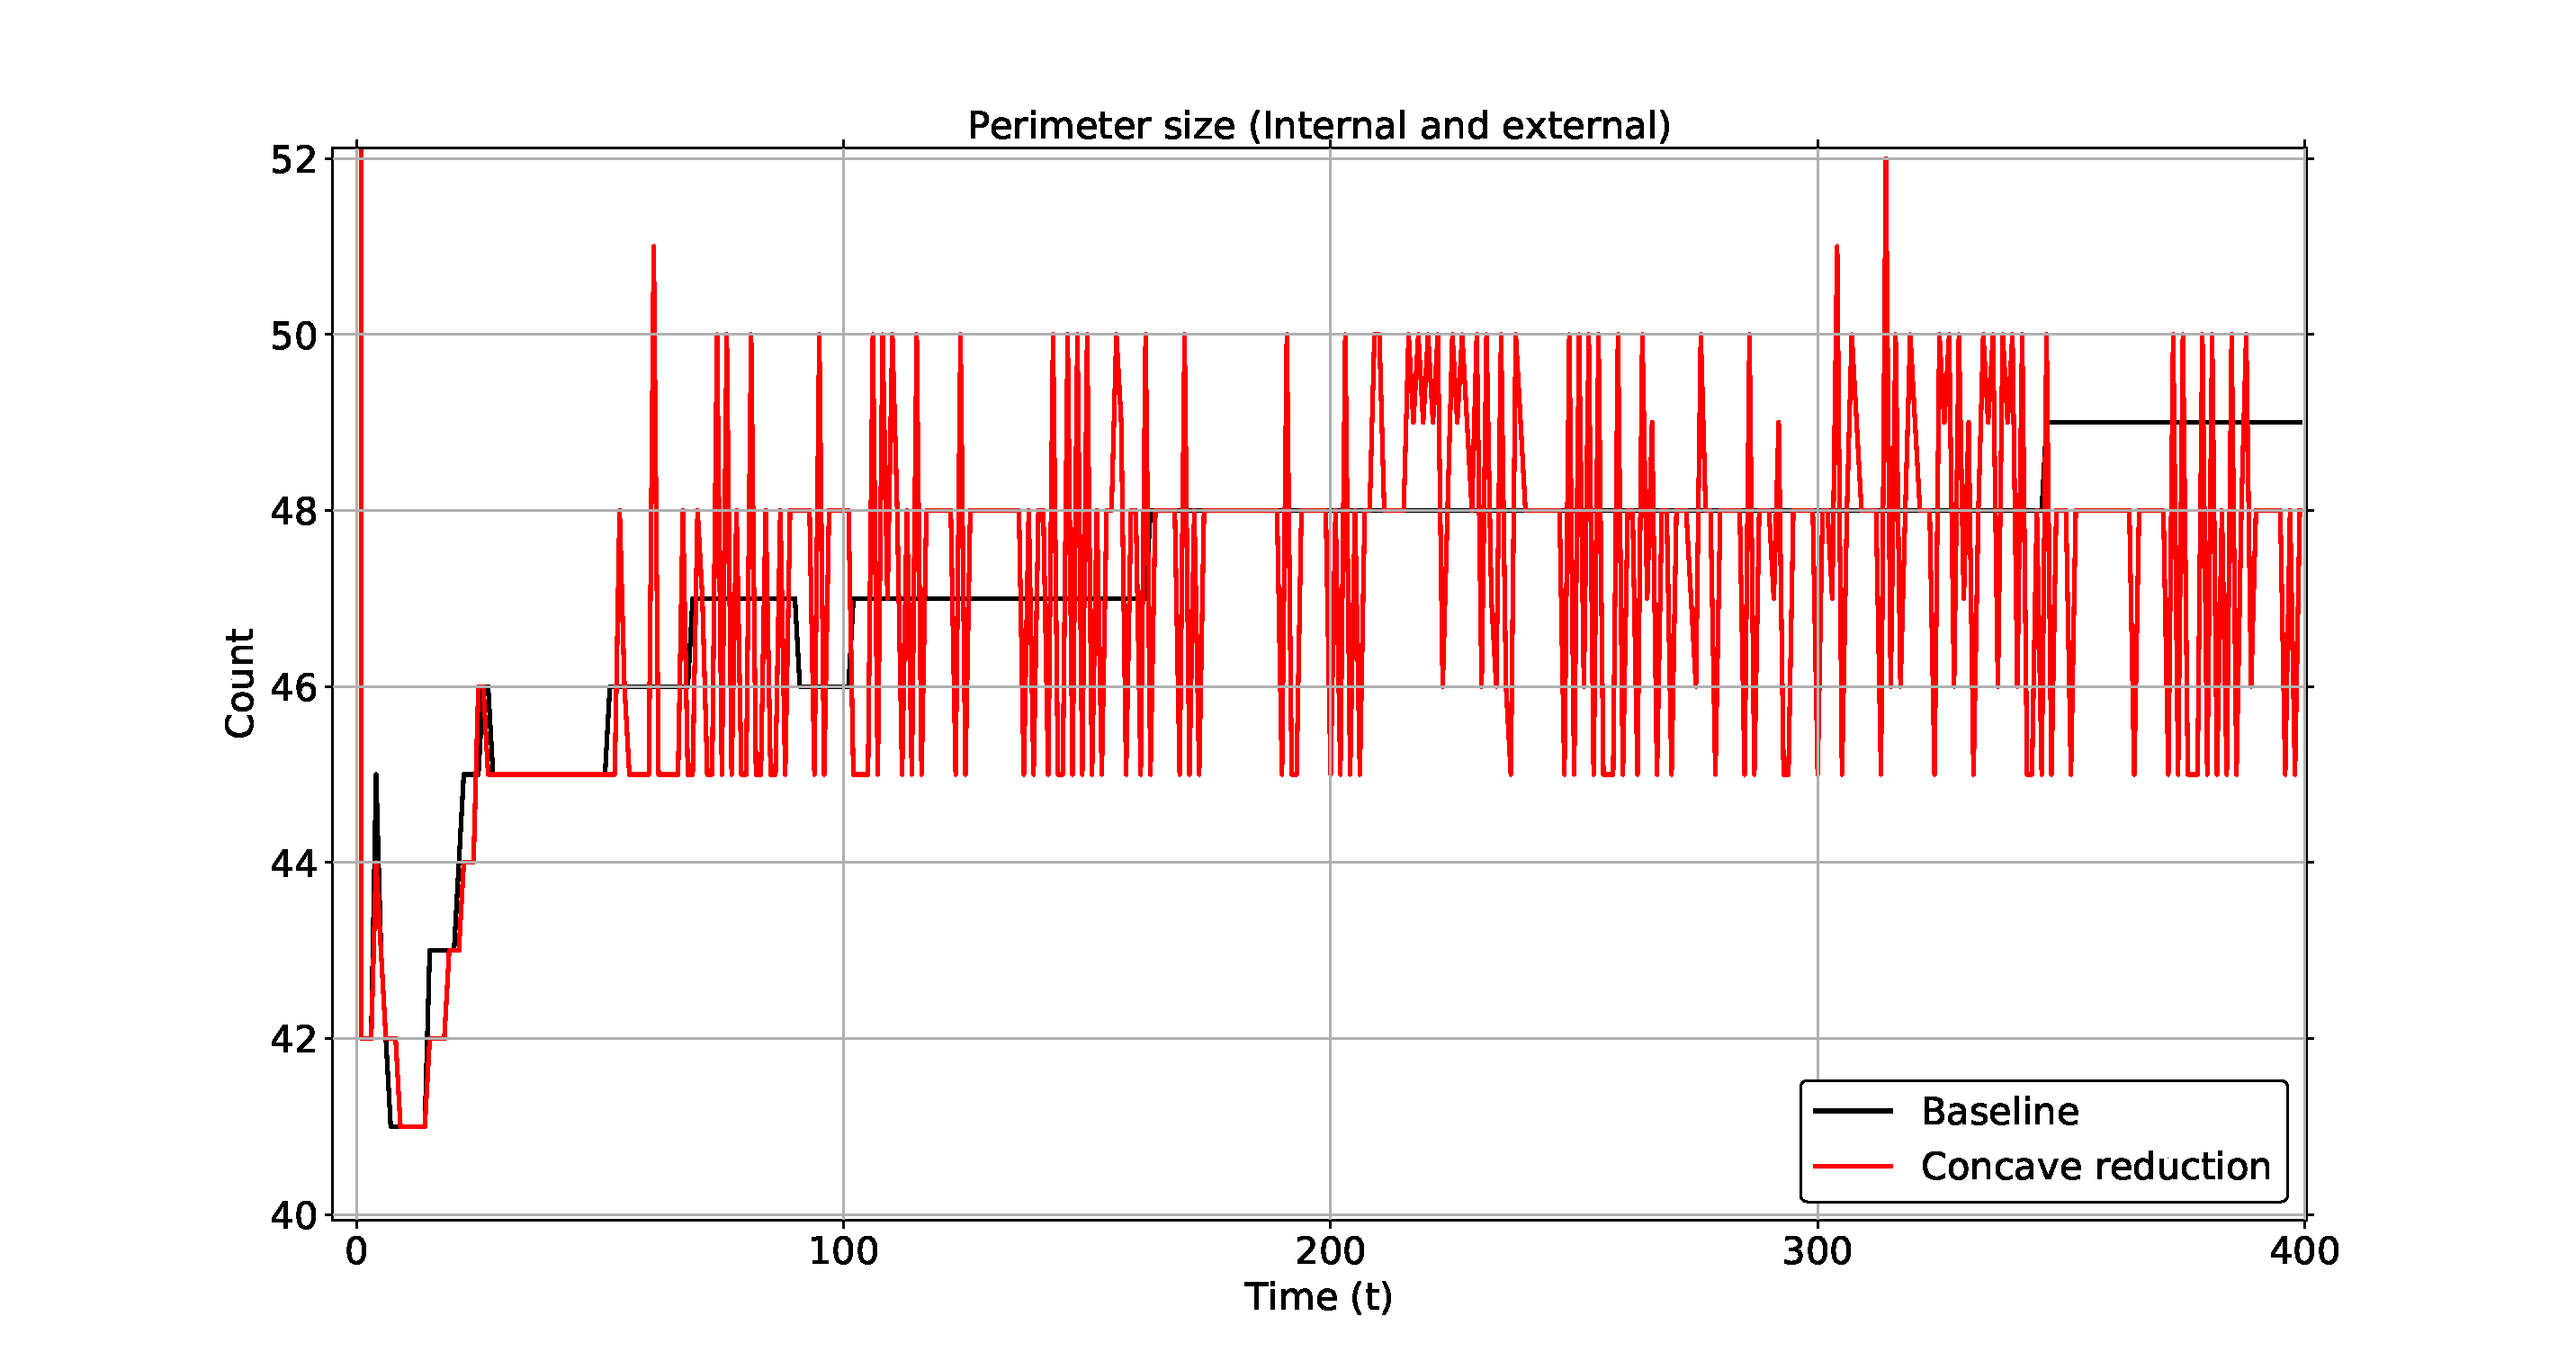
\includegraphics[width=14cm]{CHAPTER-7/figures/BaselineConcavePerimeter8060}
\end{center}
\caption{Baseline/Concave perimeter size (cohesion field 80 / repulsion field 60)\label{concave:BaselineConcavePerimeter8060}}
\end{figure}

For the period of the simulation the baseline had 19049 perimeter agents and the concave reduction had 18940 which is an improvement of 0.5\% overall for the whole simulation~(Table~\ref{tab:BaselineConcaveComparison}). This is only a small change in the perimeter size but the impact on the swarm structure is significant. The \textit{concavity reduction vectors} have `pulled' the swarm into a more circular shape~(Figure~\ref{fig:SimulationEndPoints}).

\begin{table}[H]
\begin{center}
\begin{tabular}{| p{2.3cm} | p{2cm} | p{2cm} |}
\hline
\bf Neighbour / minimum & \bf Baseline \bf swarm & \bf Concave \bf reduction \\ \hline
80/60 & 19049 & 18940 \\  \hline
80/70 & 27394 & 27987 \\  \hline
\end{tabular}\caption{Comparison of perimeter size} \label{tab:BaselineConcaveComparison}
\end{center}
\end{table}

\begin{figure}[H]
\centering
\subfigure[Baseline end]{
    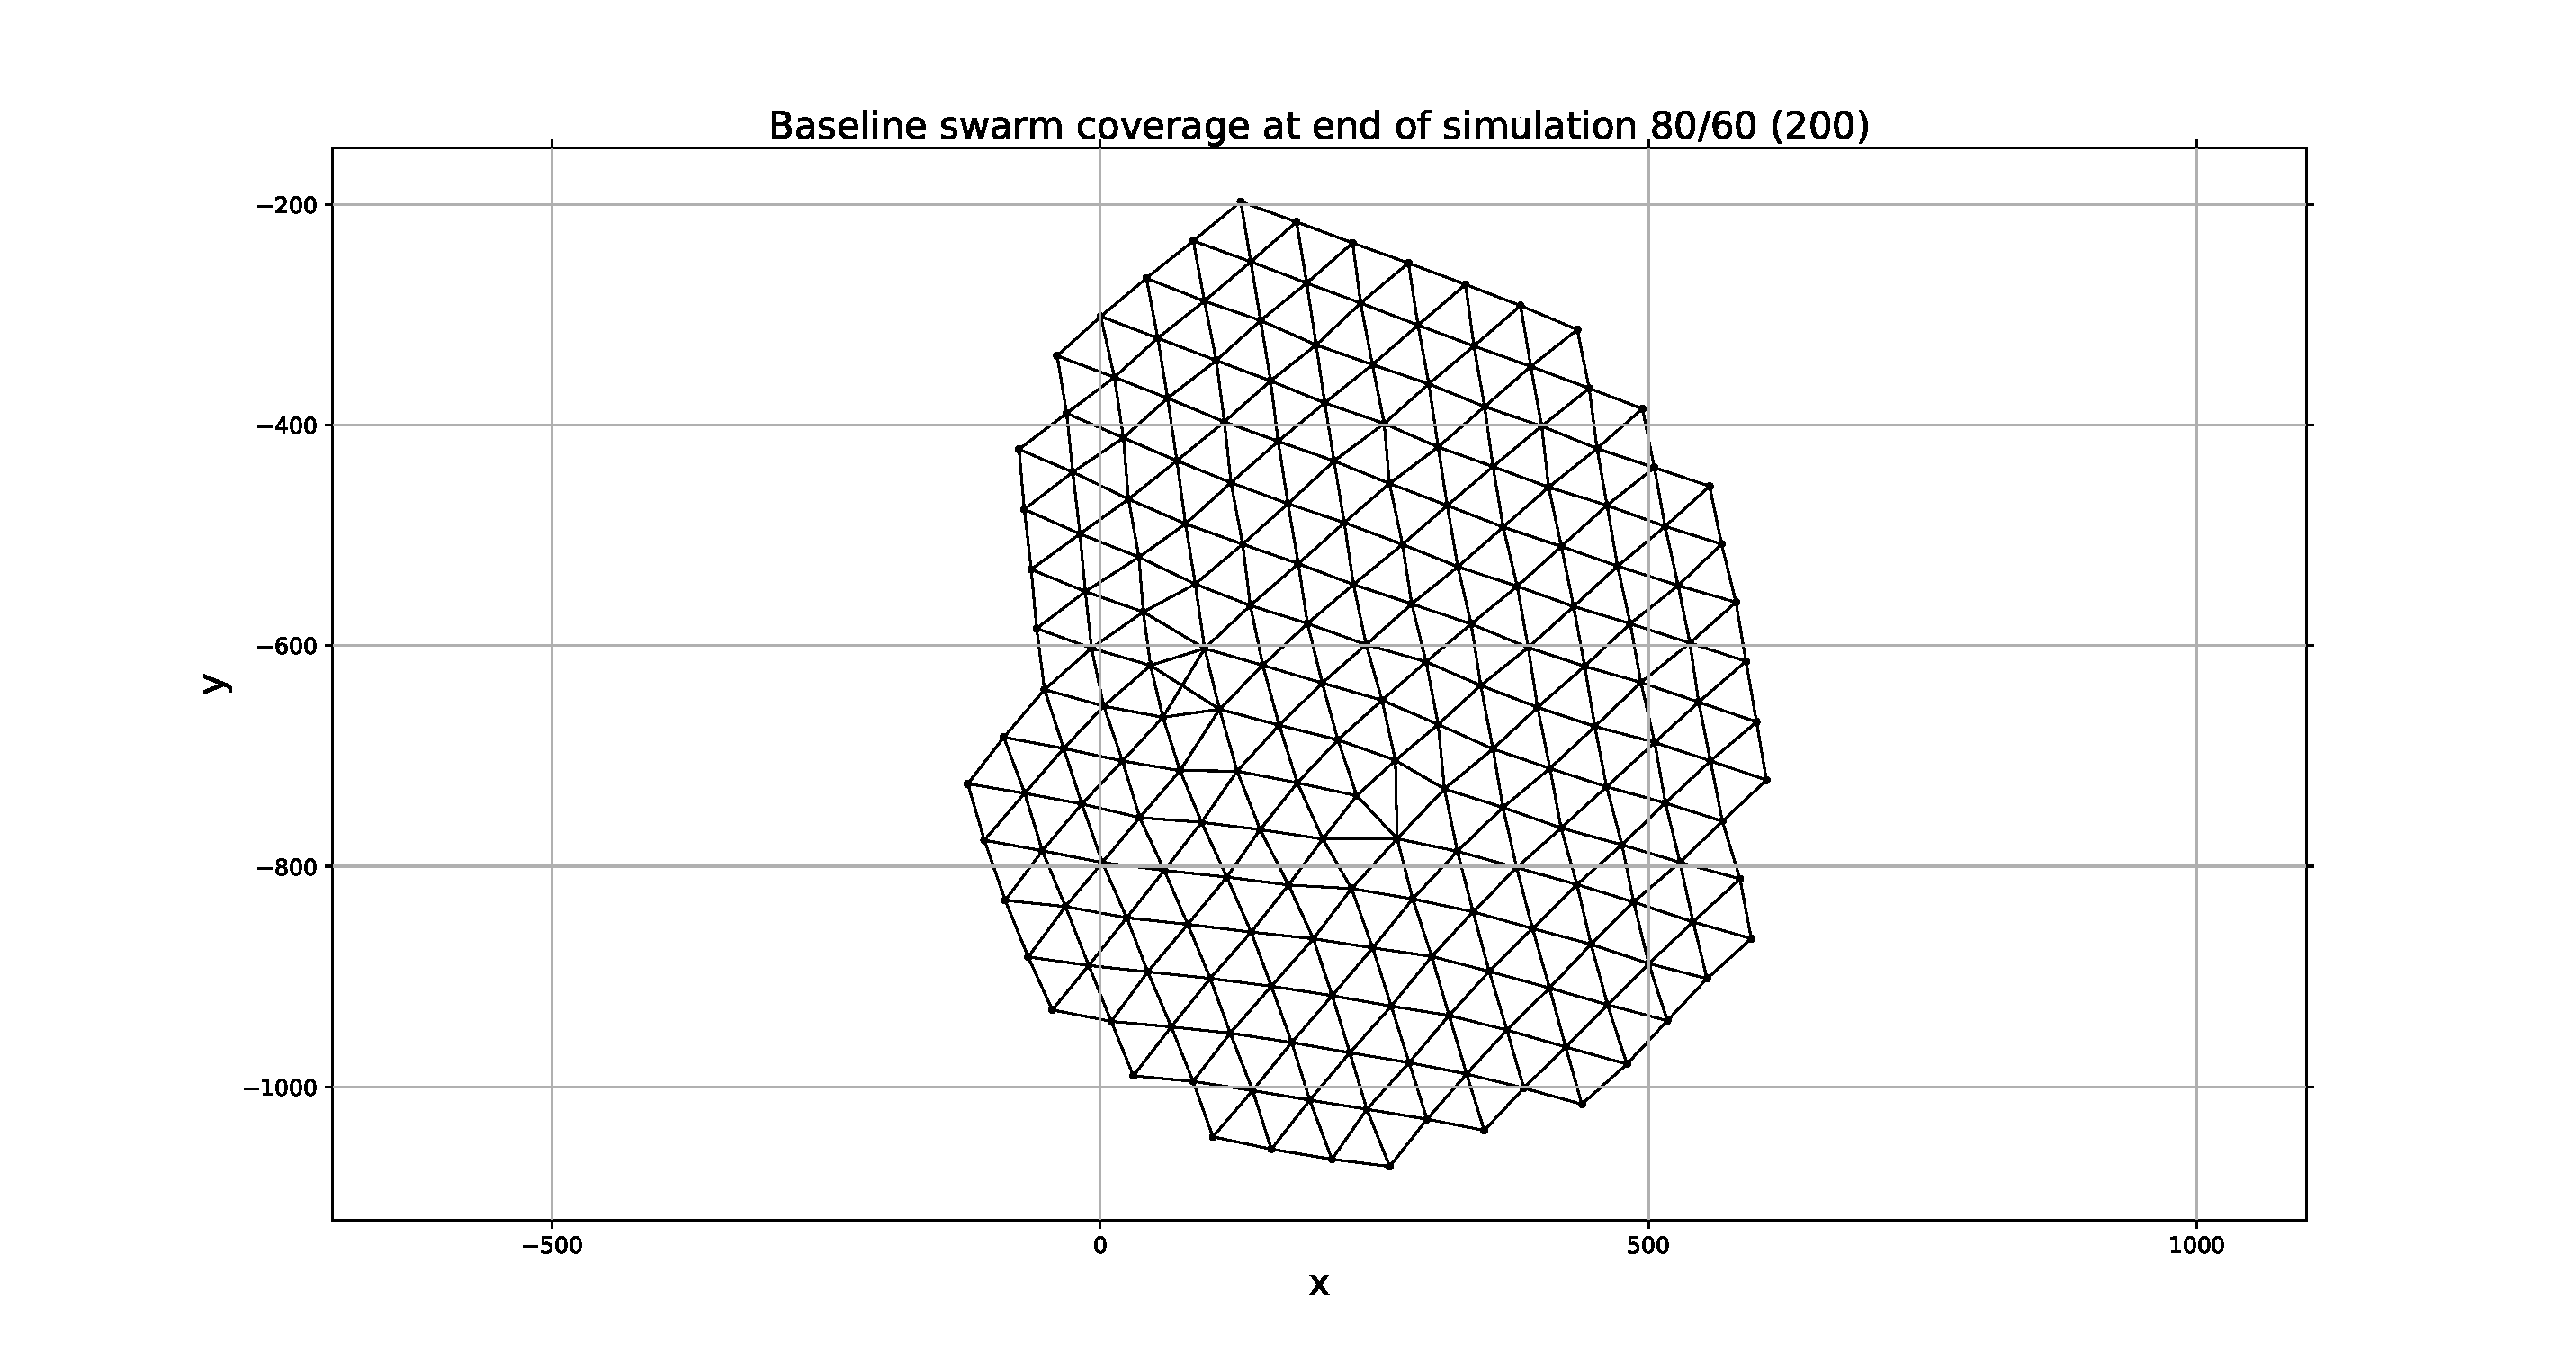
\includegraphics[width=6cm]{CHAPTER-7/figures/Baseline8060End}
    \label{fig:BaselineEndPoint}
}
\subfigure[Concave reduction end]{
    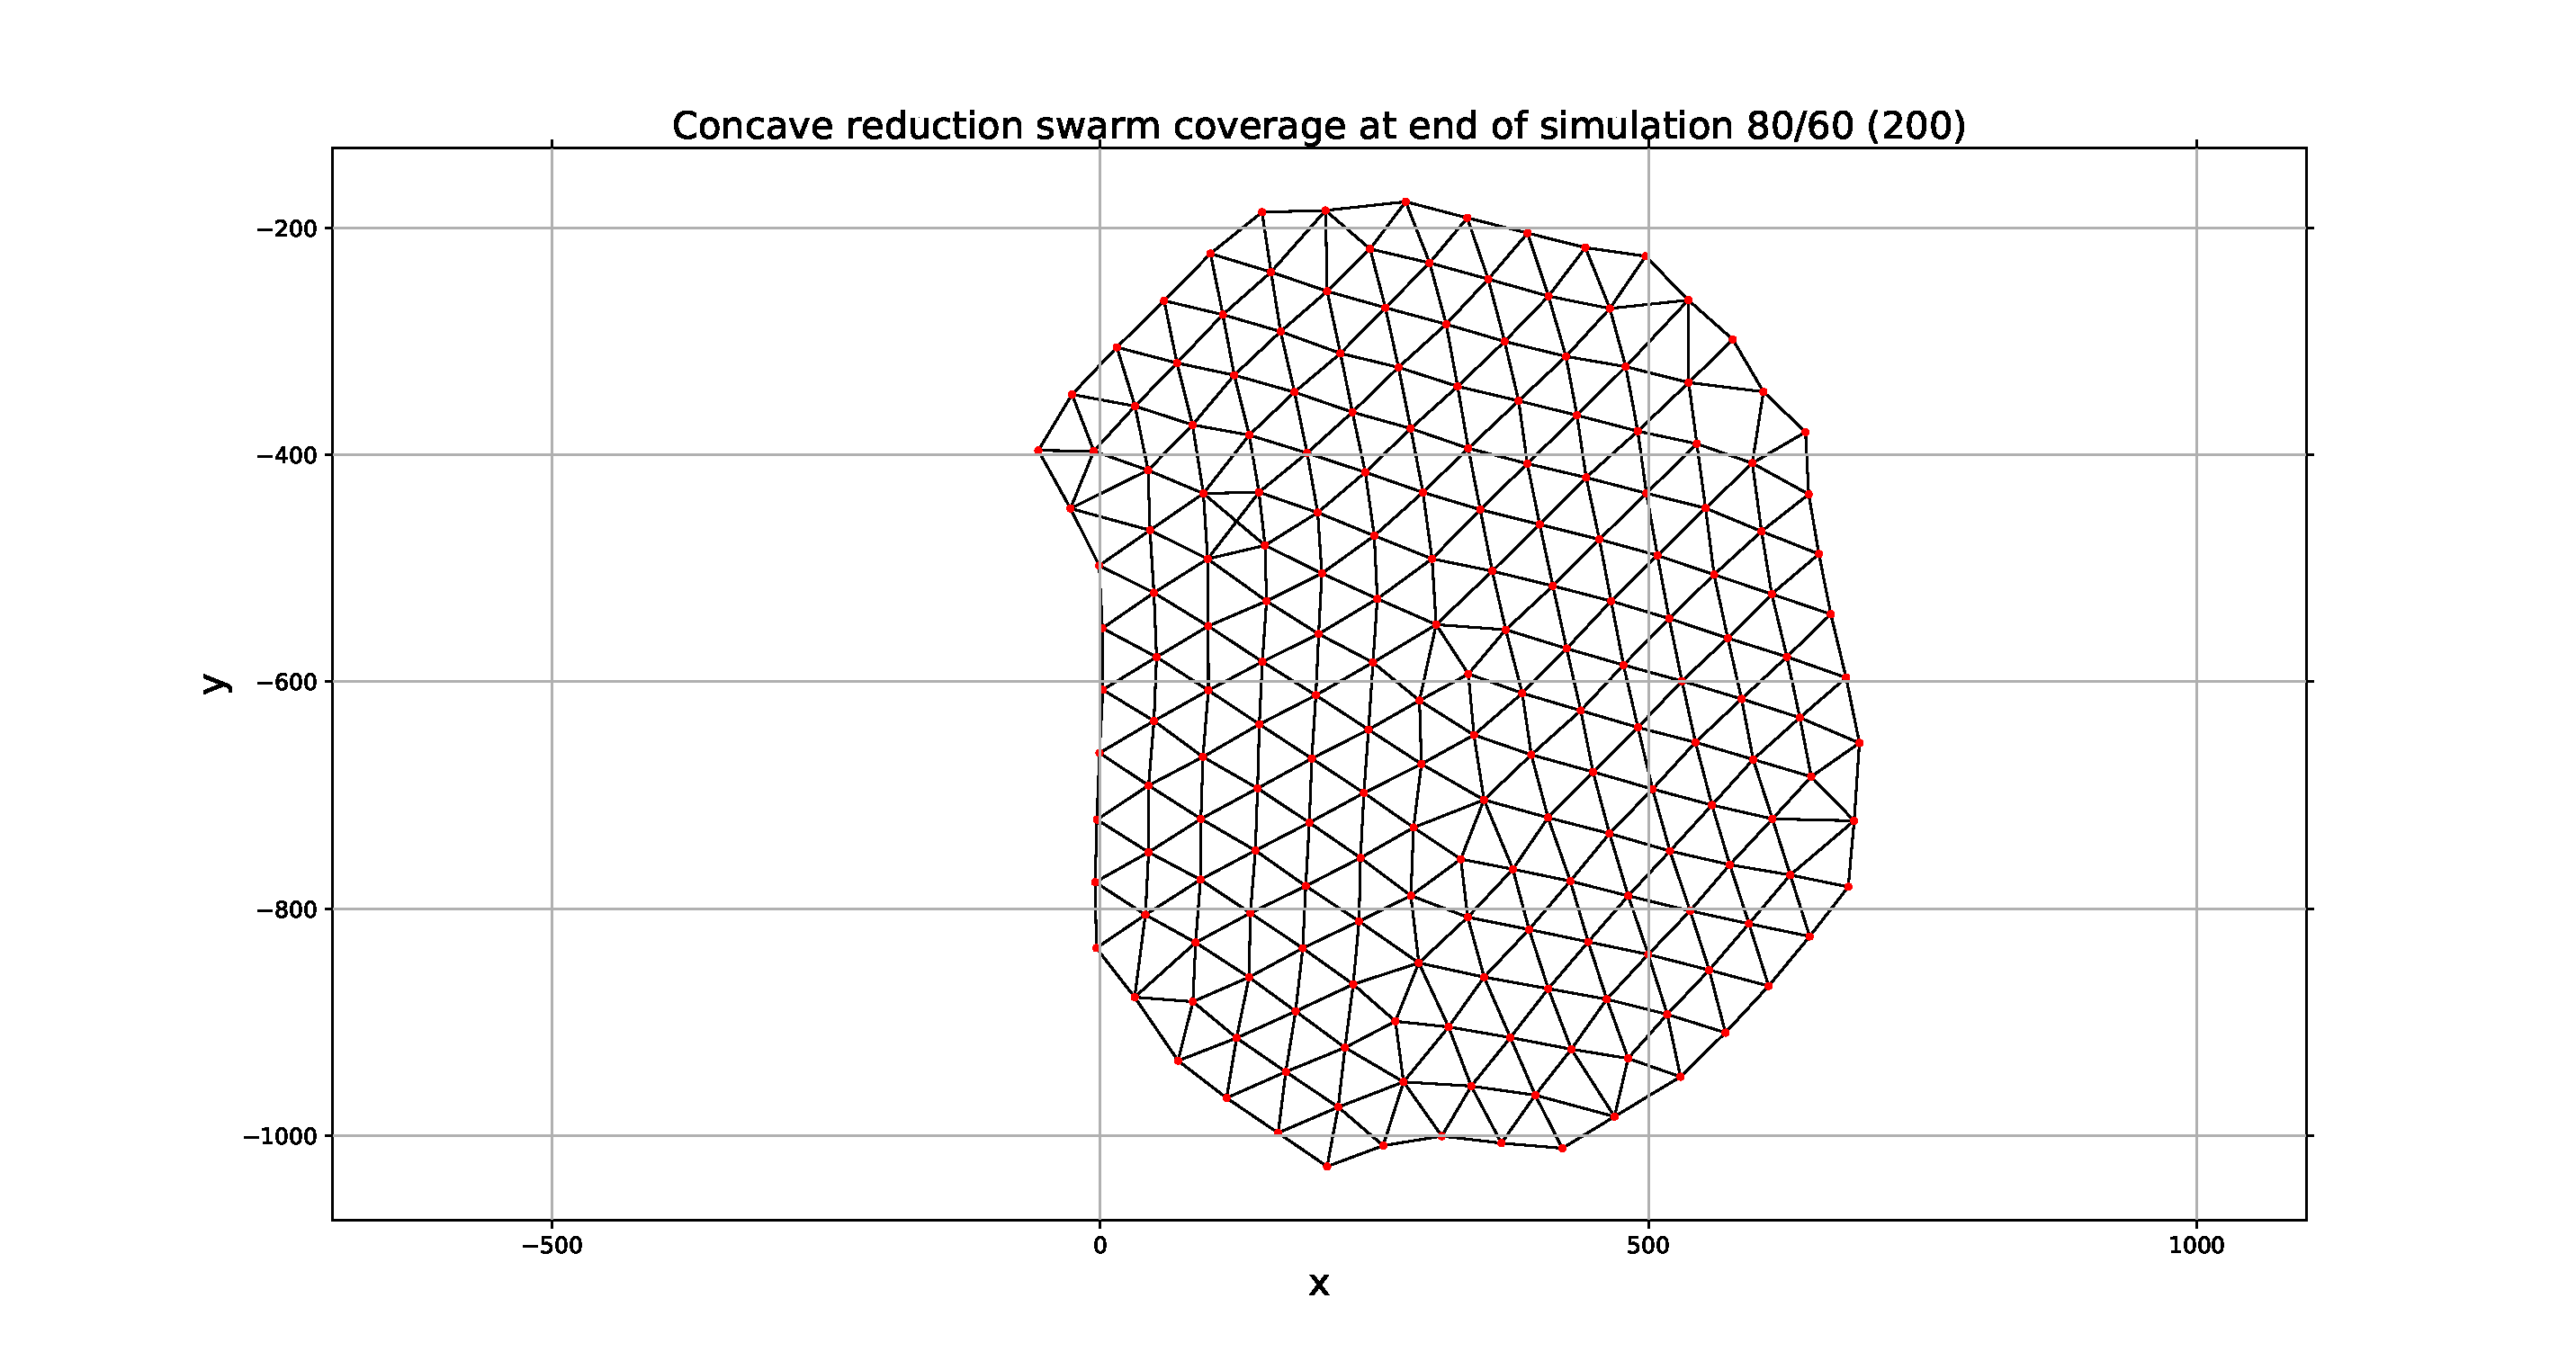
\includegraphics[width=6cm]{CHAPTER-7/figures/Concave8060End}
    \label{fig:ConcaveEndPoint}
}
\caption{Simulation end points}
\label{fig:SimulationEndPoints}
\end{figure} 

Figure~\ref{concave:BaselineConcaveEffectPath80601} shows the paths of the agents in the swarm with concave reduction (red) and without (black). The paths are similar as the swarm expands due to the \textit{repulsion vectors} being large and masking the \textit{concavity reduction vectors} due to the resultant \textit{movement vector} directing the agents in a similar direction. Once the swarm has expanded the \textit{concavity reduction vectors} create a more spherical appearance to the swarm. The \textit{concavity reduction vector magnitudes} are significantly large enough now to create a slight directional bias as shown in both~Figures~\ref{concave:BaselineConcaveEffectPath80601} and~\ref{concave:BaselineConcaveEffectPath80602}. This effect is the result of the \textit{concavity reduction vectors} pushing the anomalies on the left of the swarm resulting in the swarm moving slightly to the right due to the swarm having fewer anomalies on the opposite side of the swarm. The anomalies can be seen in~figure~\ref{concave:BaselineConcaveEffectPath80601}.
%COVERBASELINE8060.py
\begin{figure}[H]
\begin{center}
\includegraphics[width=14cm]{CHAPTER-7/figures/BaselineConcaveEffectPath80601}
\end{center}
\caption{Baseline/Concave path effect (repulsion field 80 / cohesion field 60)\label{concave:BaselineConcaveEffectPath80601}}
\end{figure}
%COVERBASELINE8060.py
\begin{figure}[H]
\begin{center}
\includegraphics[width=14cm]{CHAPTER-7/figures/BaselineConcaveEffectPath80602}
\end{center}
\caption{Baseline/Concave path effect (cohesion field 80 / repulsion field 60)\label{concave:BaselineConcaveEffectPath80602}}
\end{figure}

With the tolerance levels set appropriately the impact of the concave reduction is to reduce the number of agents being identified as coordinators~(Figure~\ref{concave:mobileSwarm1}). This reduction in perimeter size is due to a reduction in the number of anomalies in the swarm. The effect of the concave reduction on a convex (outer) perimeter is limited when a swarm is deployed in an almost circular manner as there is limited space for optimisation. The effect is more pronounced when a swarm is `malformed' with large anomalies producing concave edges.

\section{Application of concave reduction on concave perimeters (voids)}\label{sec:ApplicationConcavePerimeters}
Just as a gap on a convex perimeter is affected by concave reduction so is the perimeter of a concave perimeter (a void). The effect on a concave perimeter is more pronounced due to there being a higher ratio of concave anomalies. It is possible to have no concave gaps on a convex perimeter (a circular swarm) but a concave perimeter (void) always has concave anomalies. This characteristic allows voids to be controlled. To test the effect of concave reduction on void removal a baseline must be established~(Table~\ref{tab:BaselineConcaveReduction3}).

As with the previous testing of algorithm effects the comparison needs to take into consideration jitter (inter-agent distance and \textit{inter-agent magnitude}) and the effect on the number of coordinator agents (perimeter agents). 

Figure~\ref{tab:BaselineConcaveReduction3} shows the swarm parameters for void removal by concave reduction.

\begin{table}[H]
\begin{center}
\begin{tabular}{| p{2.3cm} | p{2cm} | p{2cm} | p{5cm} |}
\hline
\bf Weight \bf component & \bf Baseline \bf swarm & \bf Concave \bf reduction & \bf Description \\ \hline
Sample rate & 100 & 100 & ms - Unit sampling interval\\  \hline
$k_{cr}$ & 0 & 100 & weight adjuster for concavity reduction vector\\  \hline
$k_c$ & 5 & 5 & weight adjuster for cohesion field\\  \hline
$k_r$ & 15 & 15 & weight adjuster for repulsion field\\  \hline
$k_d$ & 0 & 0 & weight adjuster for destination vector 0 for static baseline 100 from goal-based\\  \hline
Repulsion Boundary & 45 & 45 & units\\  \hline
Neighbour Distance & 60 & 60 & units\\  \hline
Speed & 20 & 20 & units/s\\  \hline
\end{tabular}\caption{Baseline comparison for concave reduction} \label{tab:BaselineConcaveReduction3}
\end{center}
\end{table}

Figure~\ref{fig:SimulationEndPoints4560} shows the end points for the simulations for the concave reduction experiments. Figure~\ref{fig:BaselineEndPoint4560} shows the end point for the baseline. It shows that at the end of the simulation the void within the swarm persists. This is due to the distribution of the agents being optimal for the given simulation parameters and the structures within the swarm being `stable'. Figure~\ref{fig:ConcaveEndPoint4560} shows the end point for the simulation with concave reduction enabled using the same swarm and configuration parameters. The concave reduction algorithm has removed the void from the swarm completely and the outer perimeter has been `smoothed'. 

\begin{figure}[H]
\centering
%COVERBASELINE4560-BASEEND.py
\subfigure[Baseline end]{
    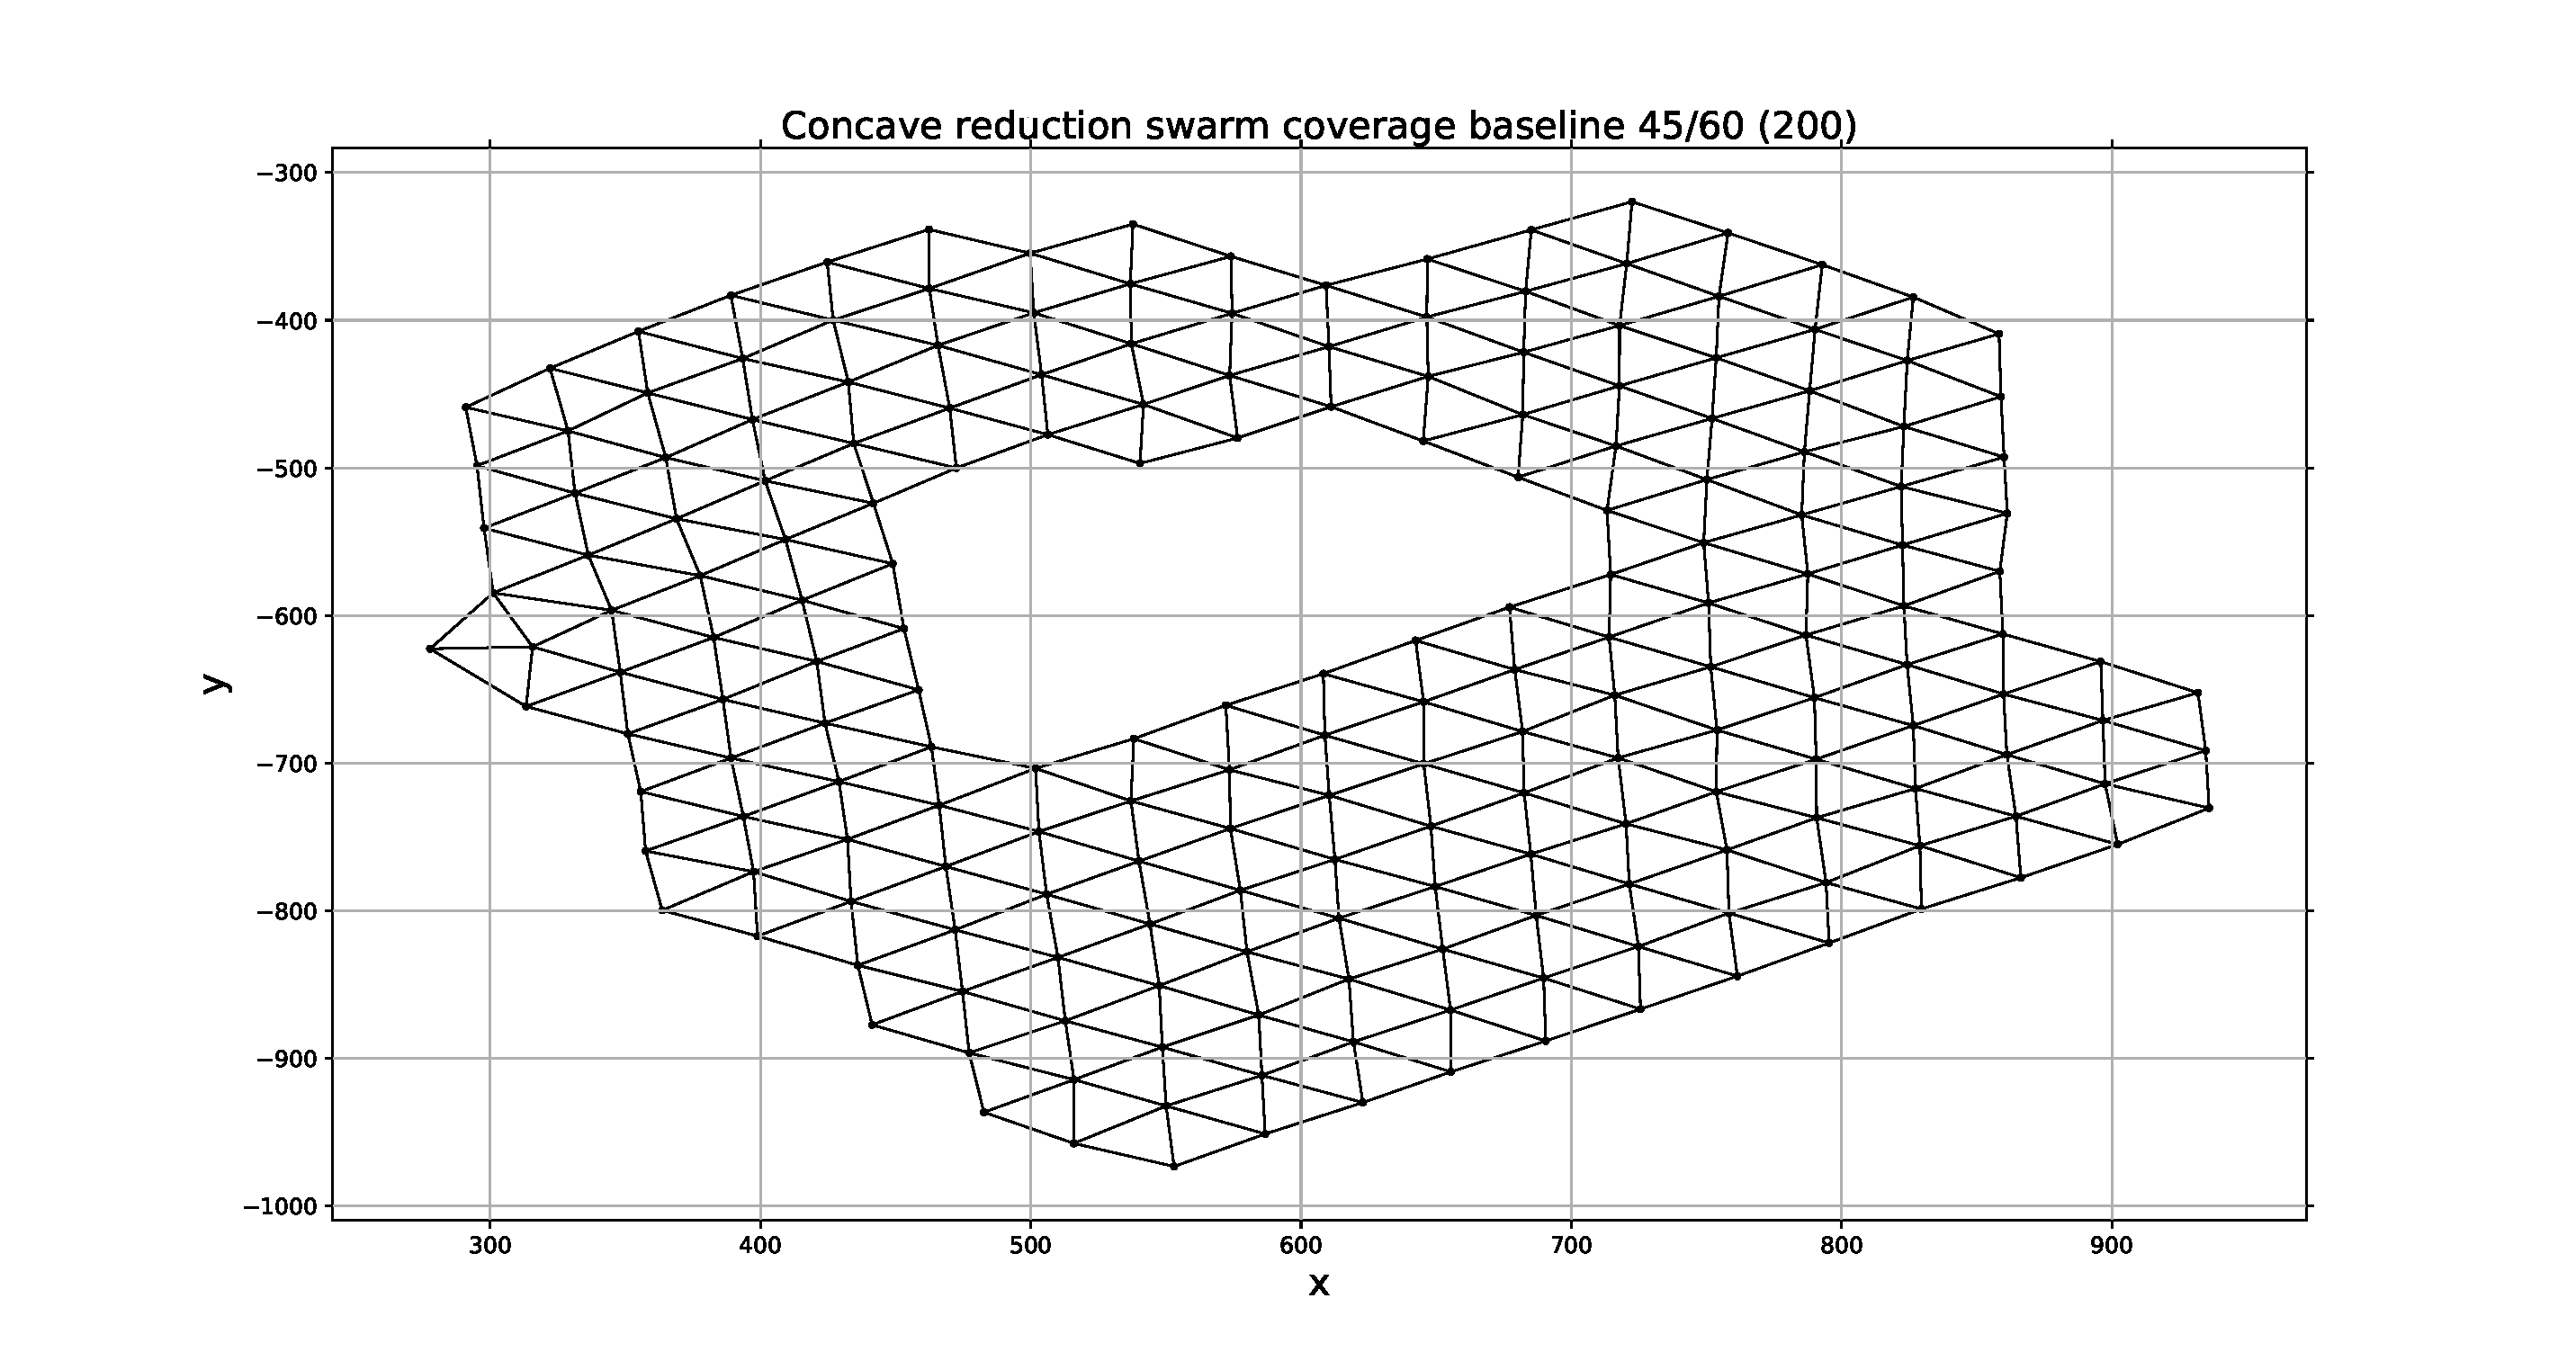
\includegraphics[width=6cm]{CHAPTER-7/figures/Baseline4560End}
    \label{fig:BaselineEndPoint4560}
}
%COVERBASELINE4560END3.py
\subfigure[Concave reduction end]{
    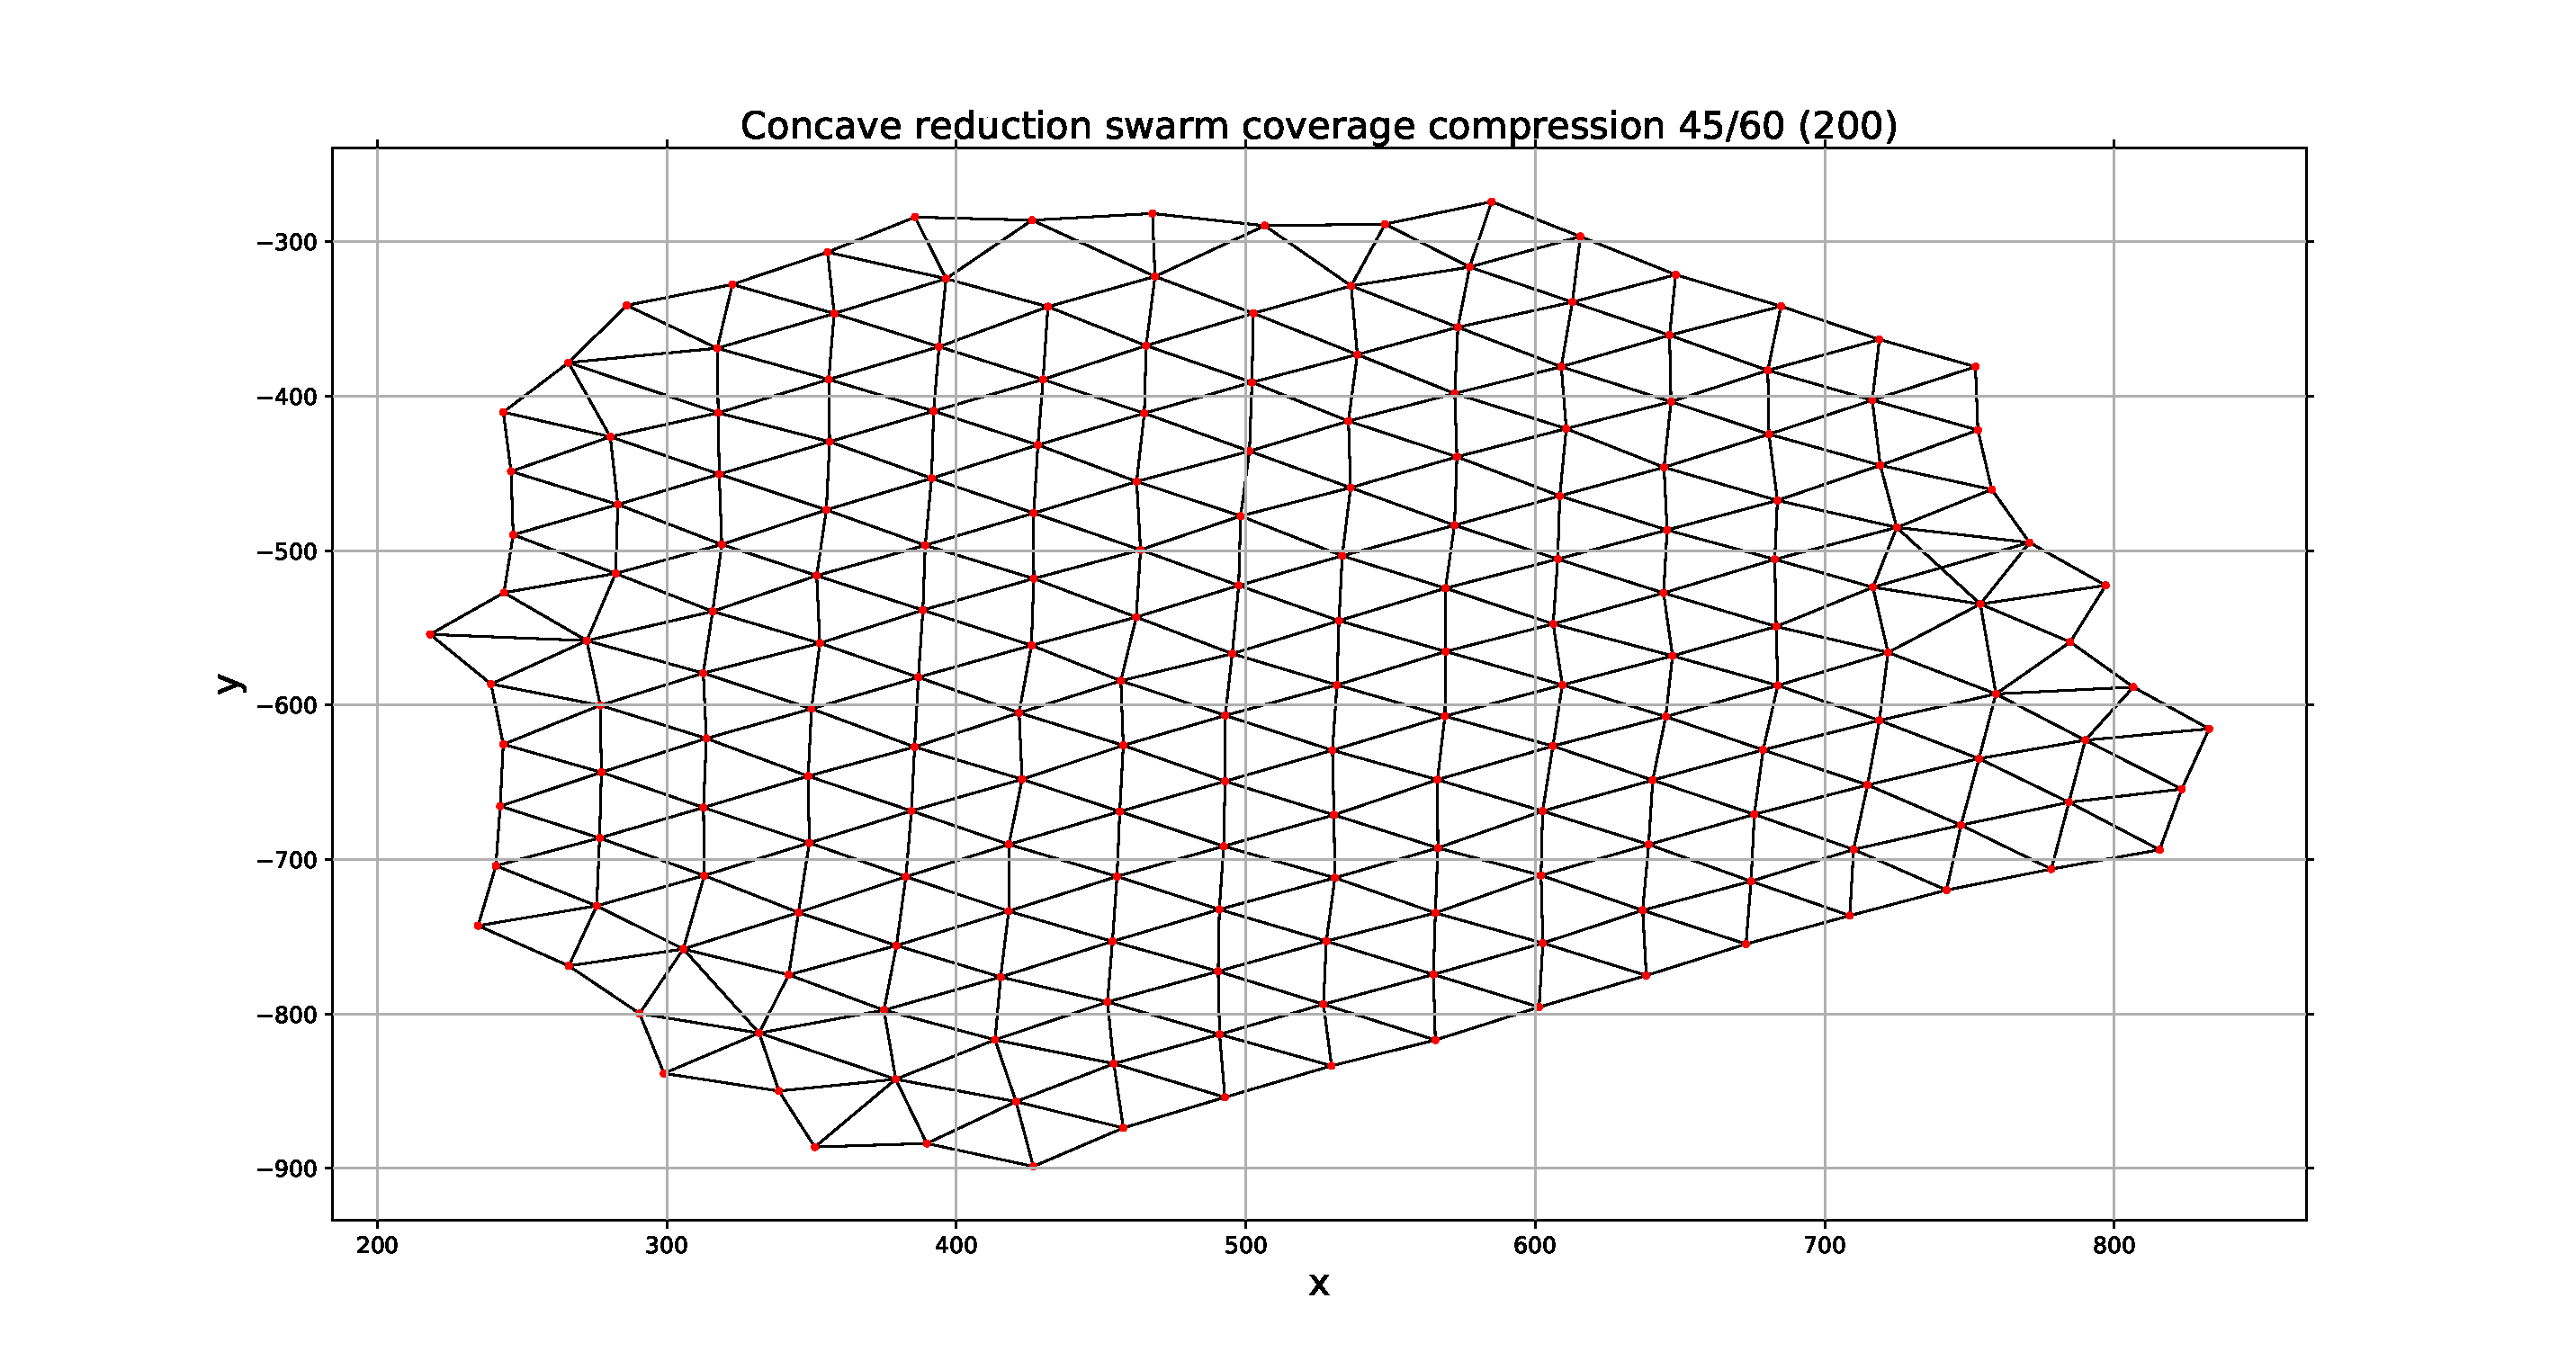
\includegraphics[width=6cm]{CHAPTER-7/figures/Concave4560End}
    \label{fig:ConcaveEndPoint4560}
}
\caption{Simulation end points}
\label{fig:SimulationEndPoints4560}
\end{figure} 

Figure~\ref{fig:VoidConcaveReduction} shows the stages that the swarm goes through when the concave reduction closes the void. The initial deployment of the baseline and concave reduction swarm are the same~(Figure~\ref{fig:VoidConcaveReduction1}). The concave reduction slowly reduces the void~(Figure~\ref{fig:VoidConcaveReduction2}) and smooths the outer perimeter. Once the smoothing begins the internal anomaly is filled from behind as the inner agents are drawn into the void. This causes small voids to `percolate' outwards through the swarm until they meet an outer perimeter. Two of these `percolating voids' can be seen in~figure~\ref{fig:VoidConcaveReduction2} to the left of the void and above the void. Once the `percolation' process has completed the void is closed~(Figure~\ref{fig:VoidConcaveReduction3}). The swarm edges also take on a more `rounded' appearance caused by the edges of the swarm being `pulled' to create a convex edge.

\begin{figure}[H]
\centering
%COVERBASELINE4560END1.py
\subfigure[Initial]{
    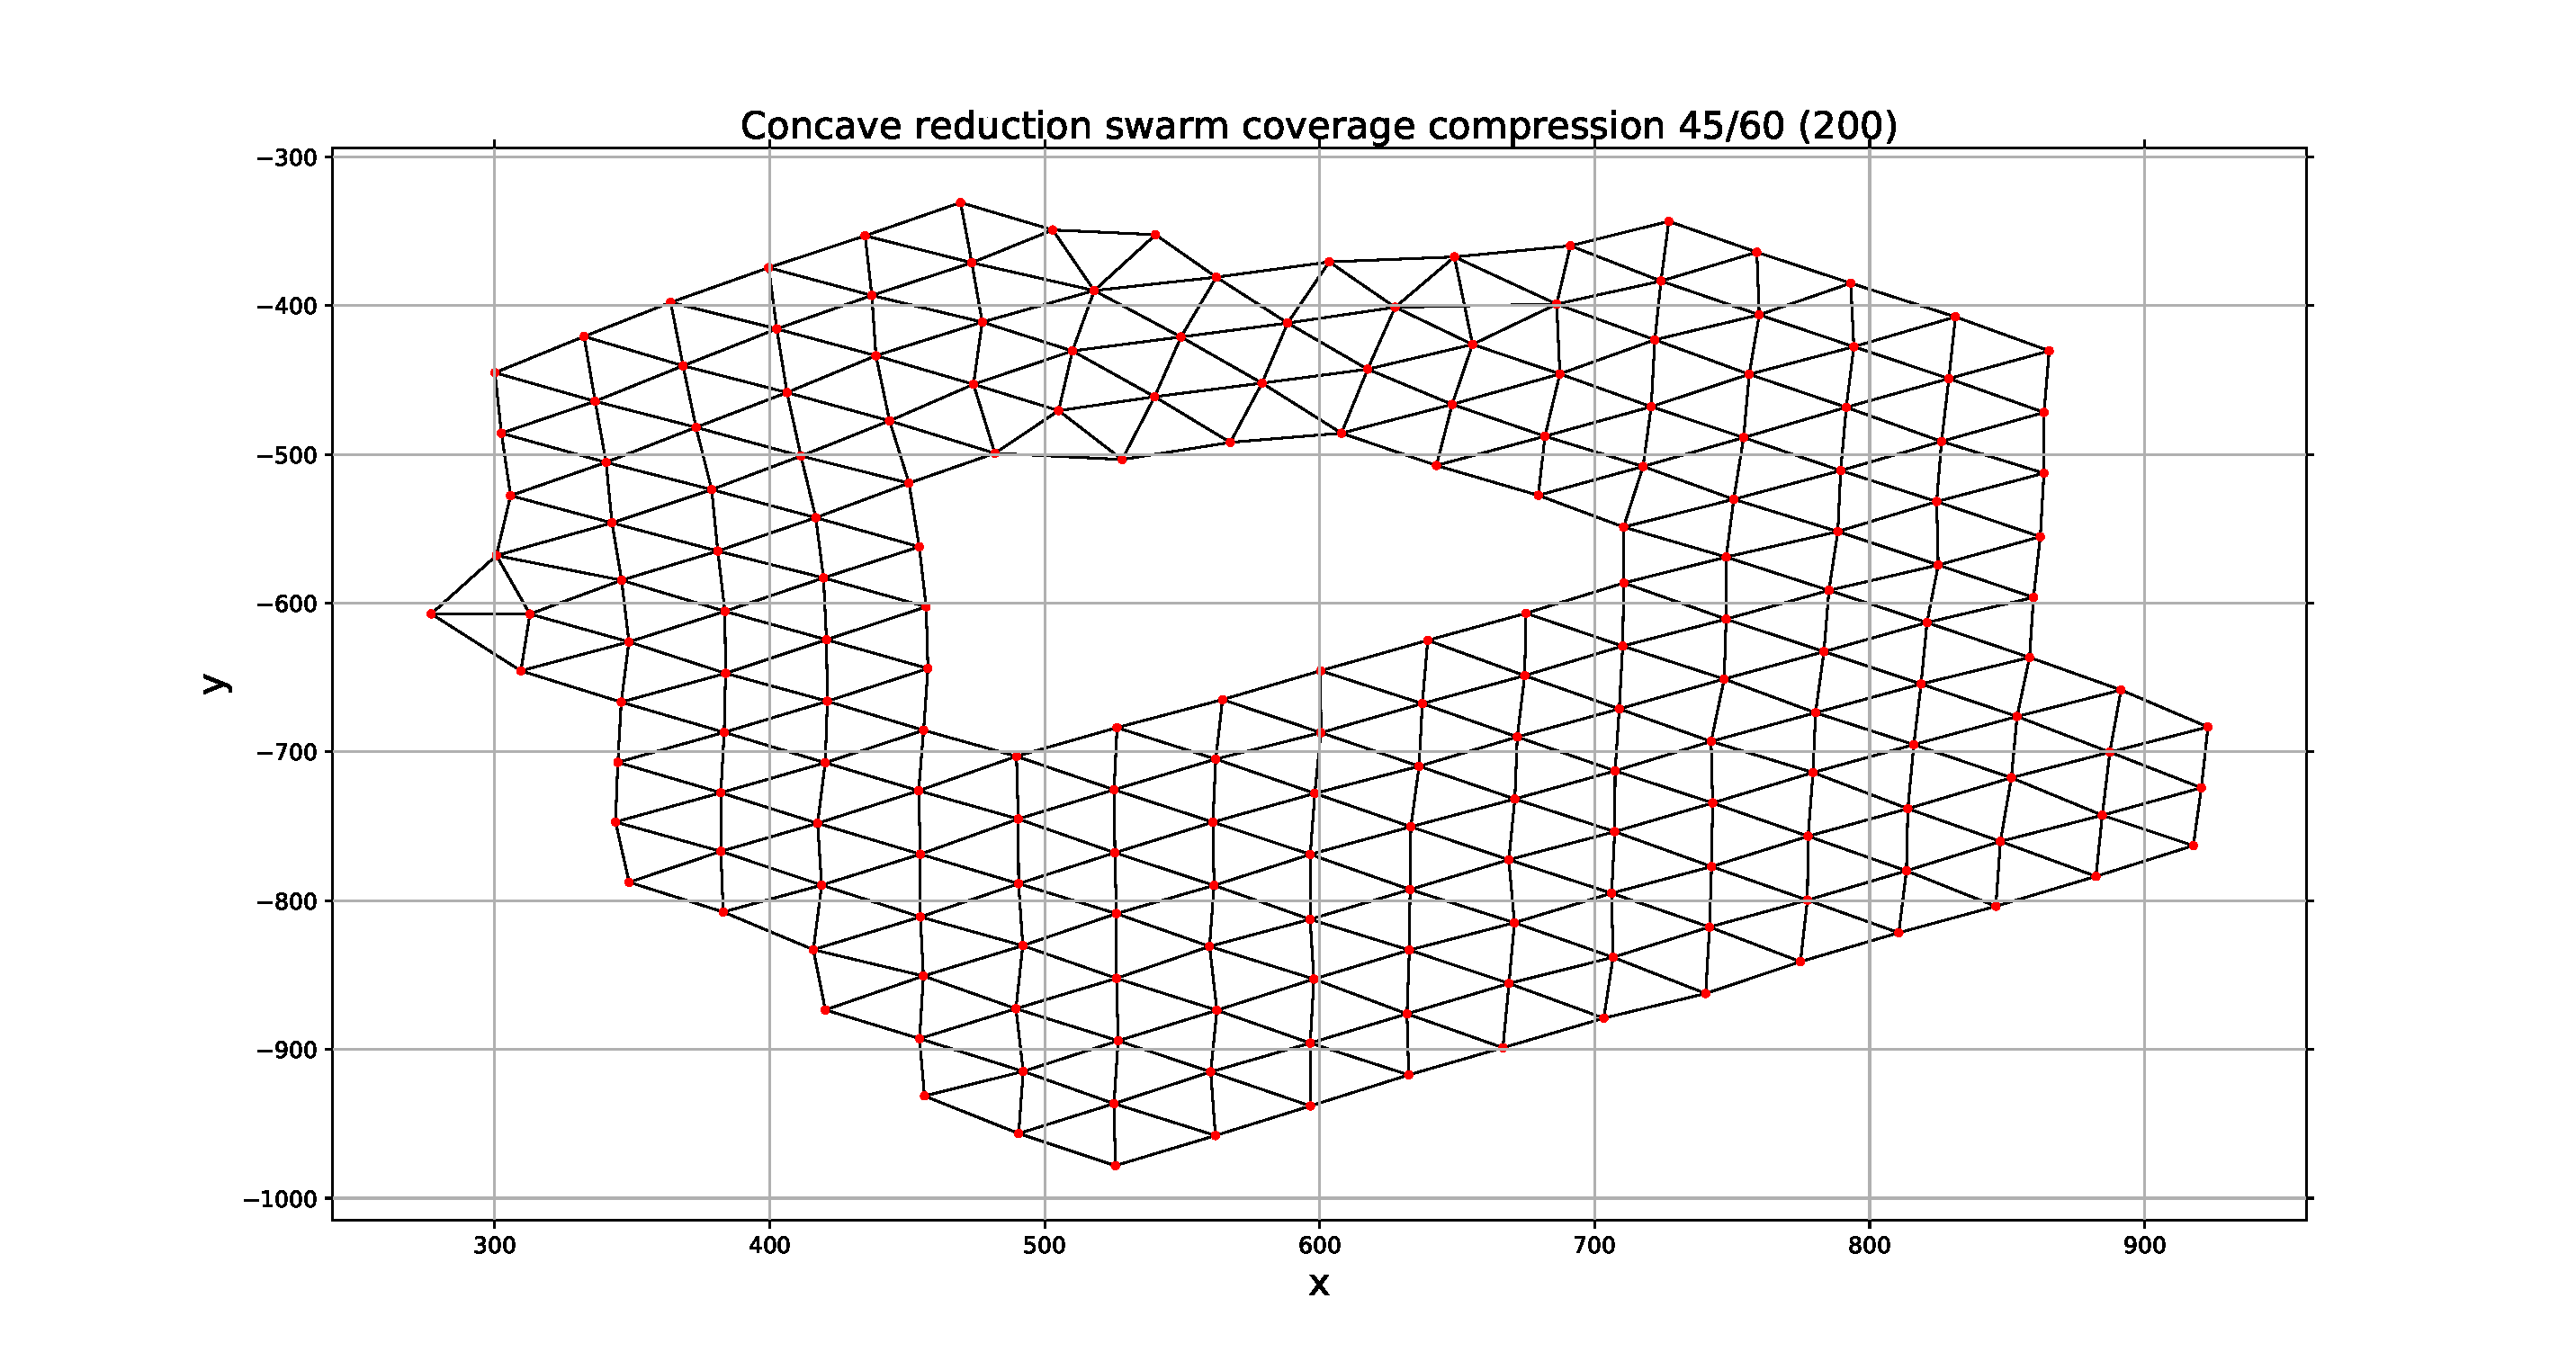
\includegraphics[width=6cm]{CHAPTER-7/figures/Concave4560-1}
    \label{fig:VoidConcaveReduction1}
}
%COVERBASELINE4560END2.py
\subfigure[Partial]{
    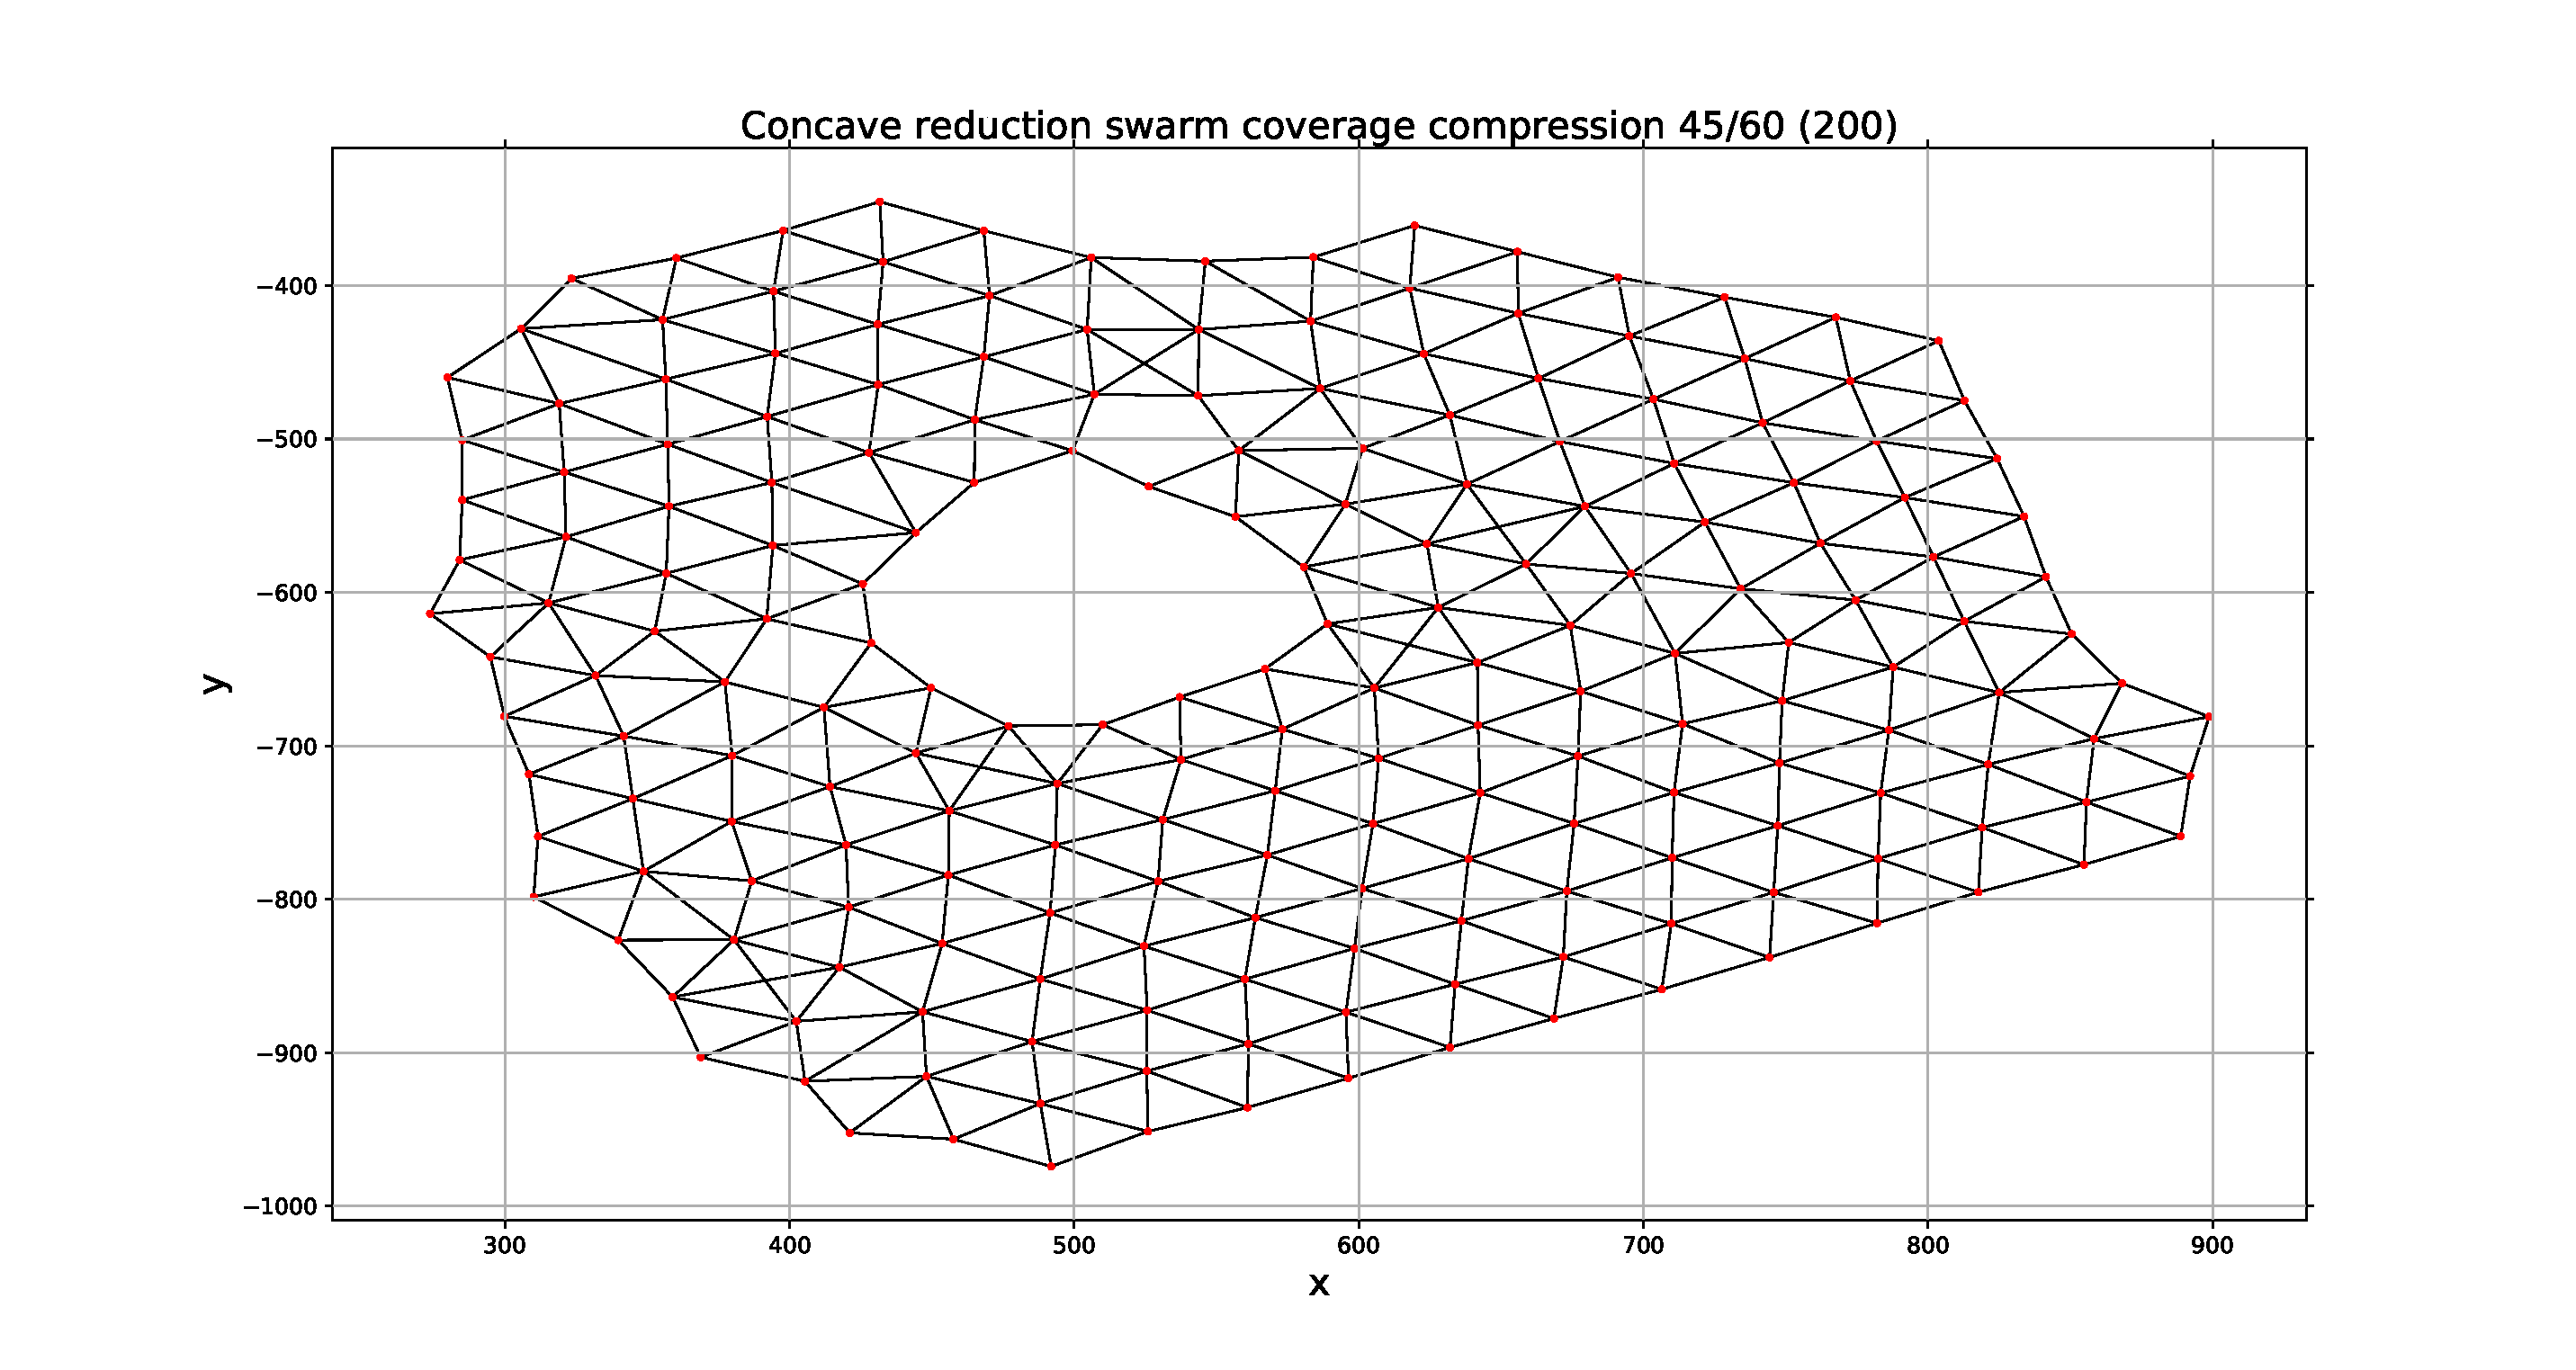
\includegraphics[width=6cm]{CHAPTER-7/figures/Concave4560-2}
    \label{fig:VoidConcaveReduction2}
}
%COVERBASELINE4560END3.py
\subfigure[Complete]{
    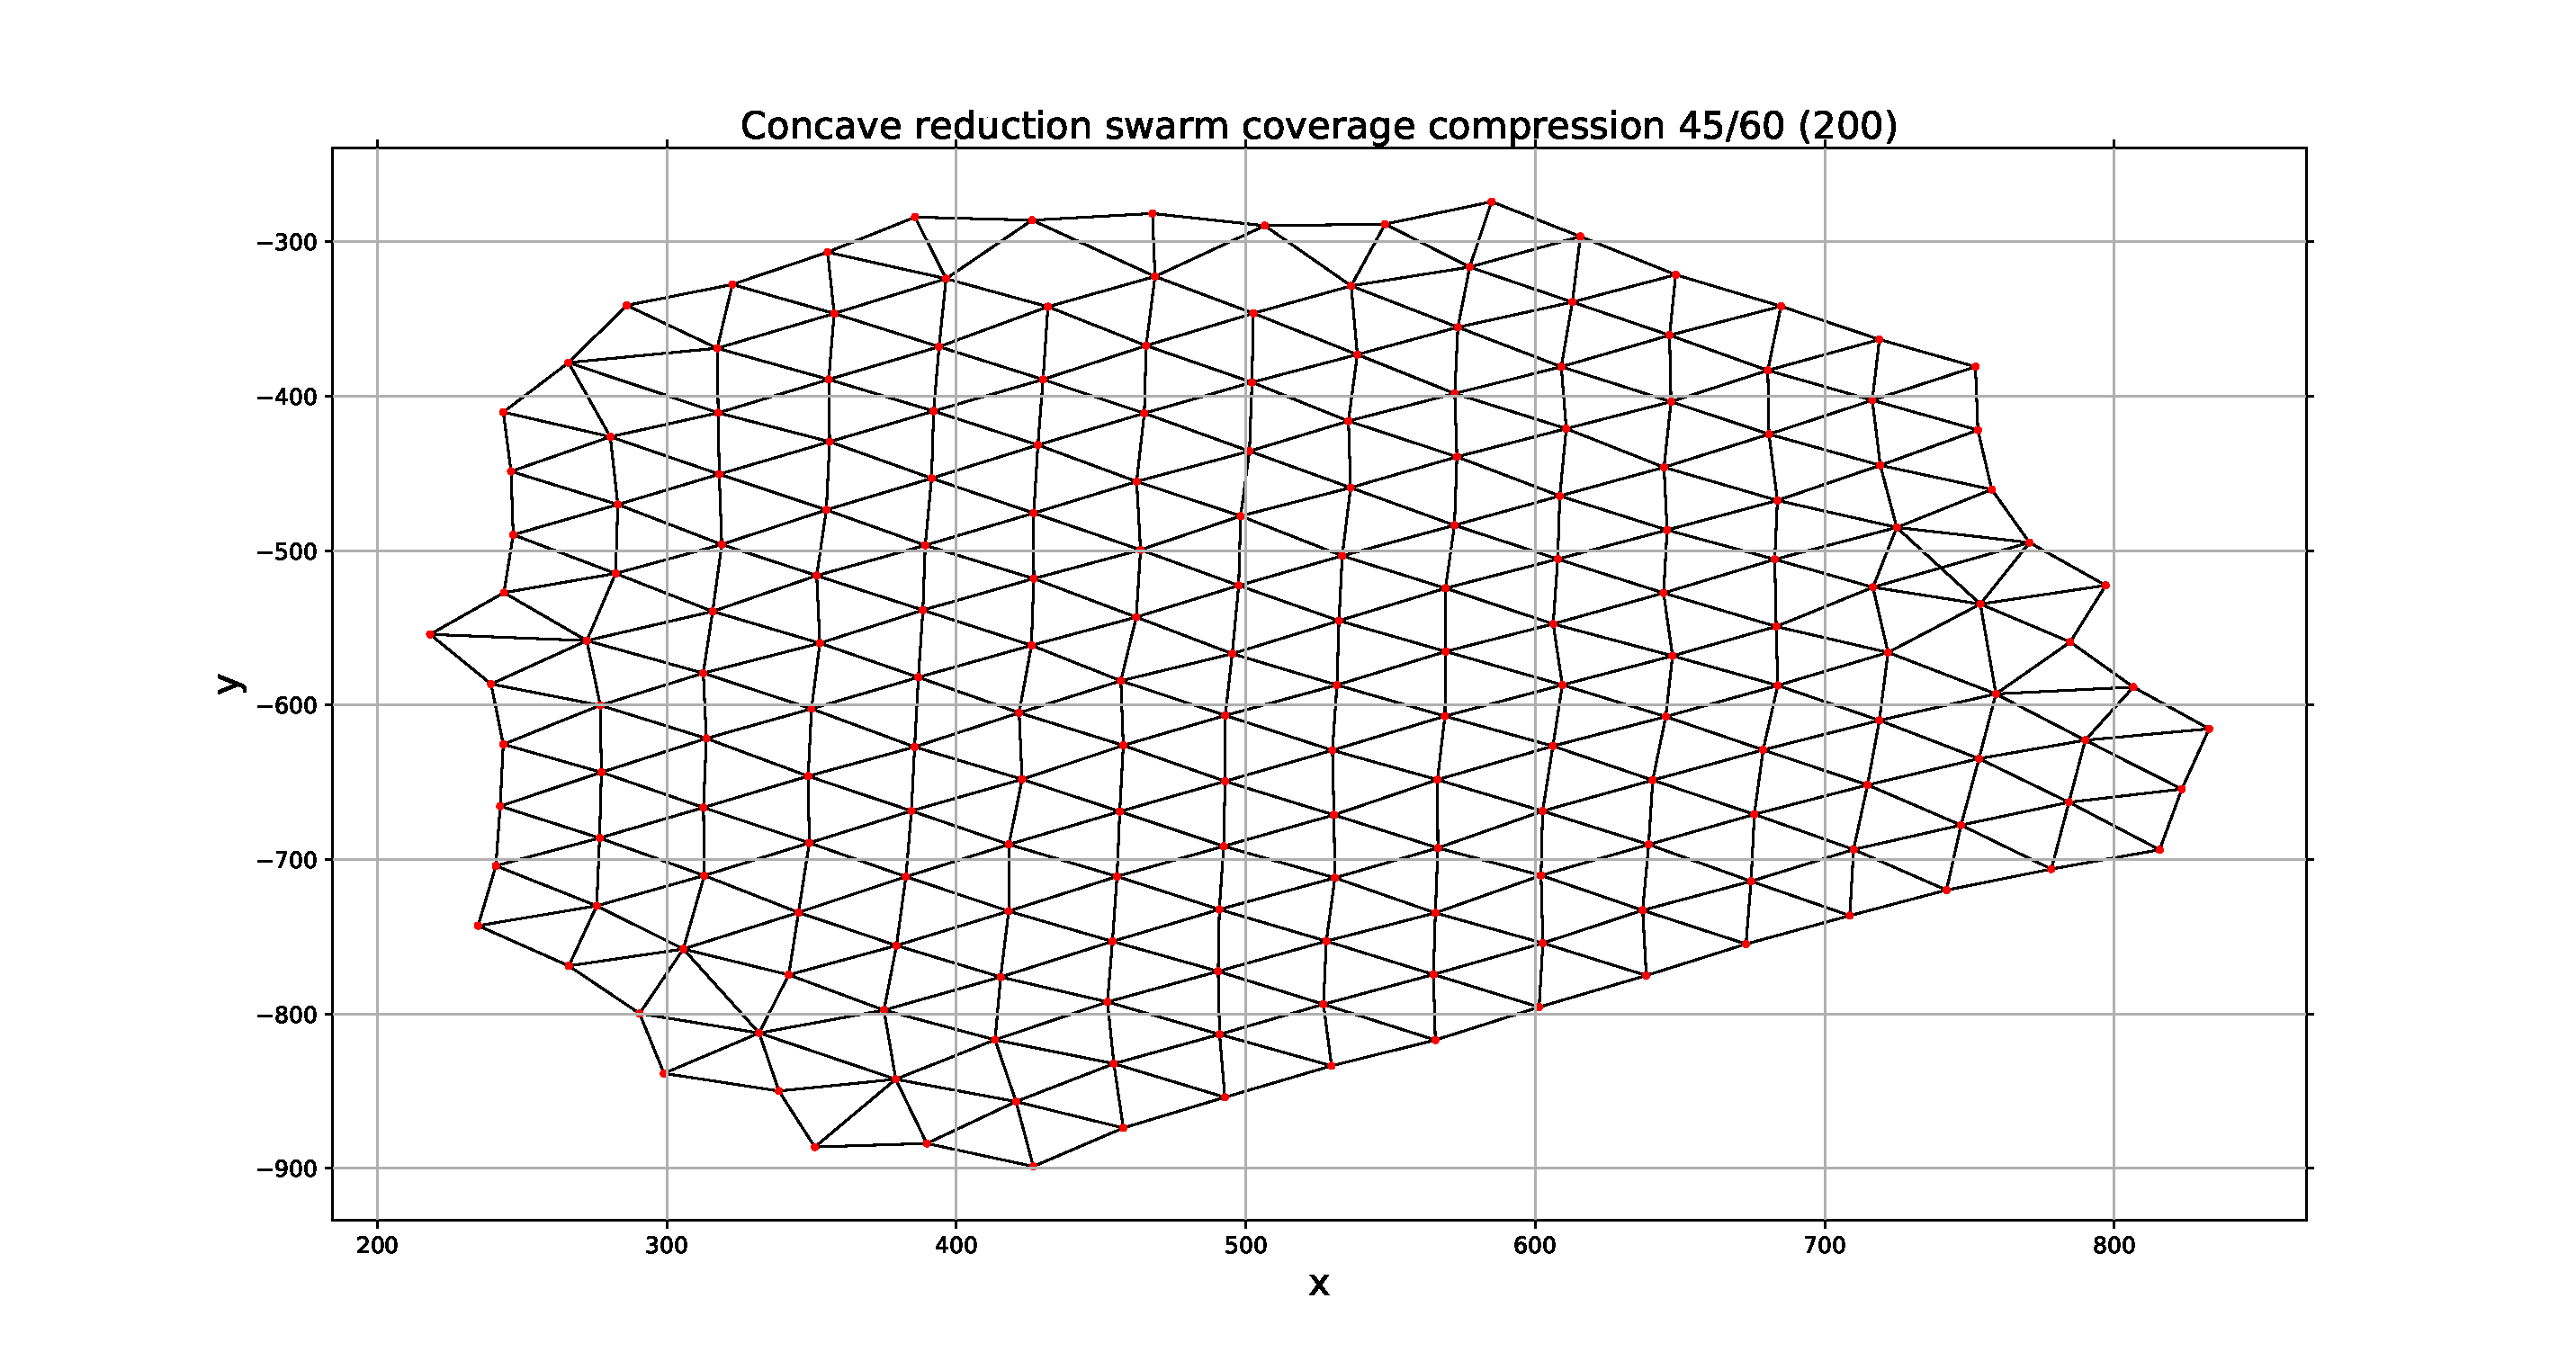
\includegraphics[width=6cm]{CHAPTER-7/figures/Concave4560-3}
    \label{fig:VoidConcaveReduction3}
}
\caption[200 agent swarm with void]{200 agent swarm with void}
\label{fig:VoidConcaveReduction}
\end{figure}

Figures \ref{voids:ConcavePerimeter4560-DIST}, \ref{voids:ConcavePerimeter4560-DIST-2}, \ref{voids:ConcavePerimeter4560-MAG}, \ref{voids:ConcavePerimeter4560-MAG-2} show the effect the concave reduction has on the inter-agent distances and \textit{inter-agent vector magnitudes} for the simulation. 

Figure~\ref{voids:ConcavePerimeter4560-DIST} shows that the process of reducing the void increases the average distance of the agents. This is caused by the concave agents `pulling' away from their neighbours. The baseline experiment shows a limited change in the variance (jitter) due to the swarm being close to stable even though there is a void present. 

The concave reduction algorithm creates a more pronounced variation due to the void having multiple anomalies. The concave reduction process closes the void over a period of 3 seconds and the swarm then settles to a steady average distance with a stable variance. The increased variance up to 3 seconds is the `percolation' of the internal anomalies to the outer perimeter as the void is closed.
%SWARMHOLE-DIST-4560.py
\begin{figure}[H]
\begin{center}
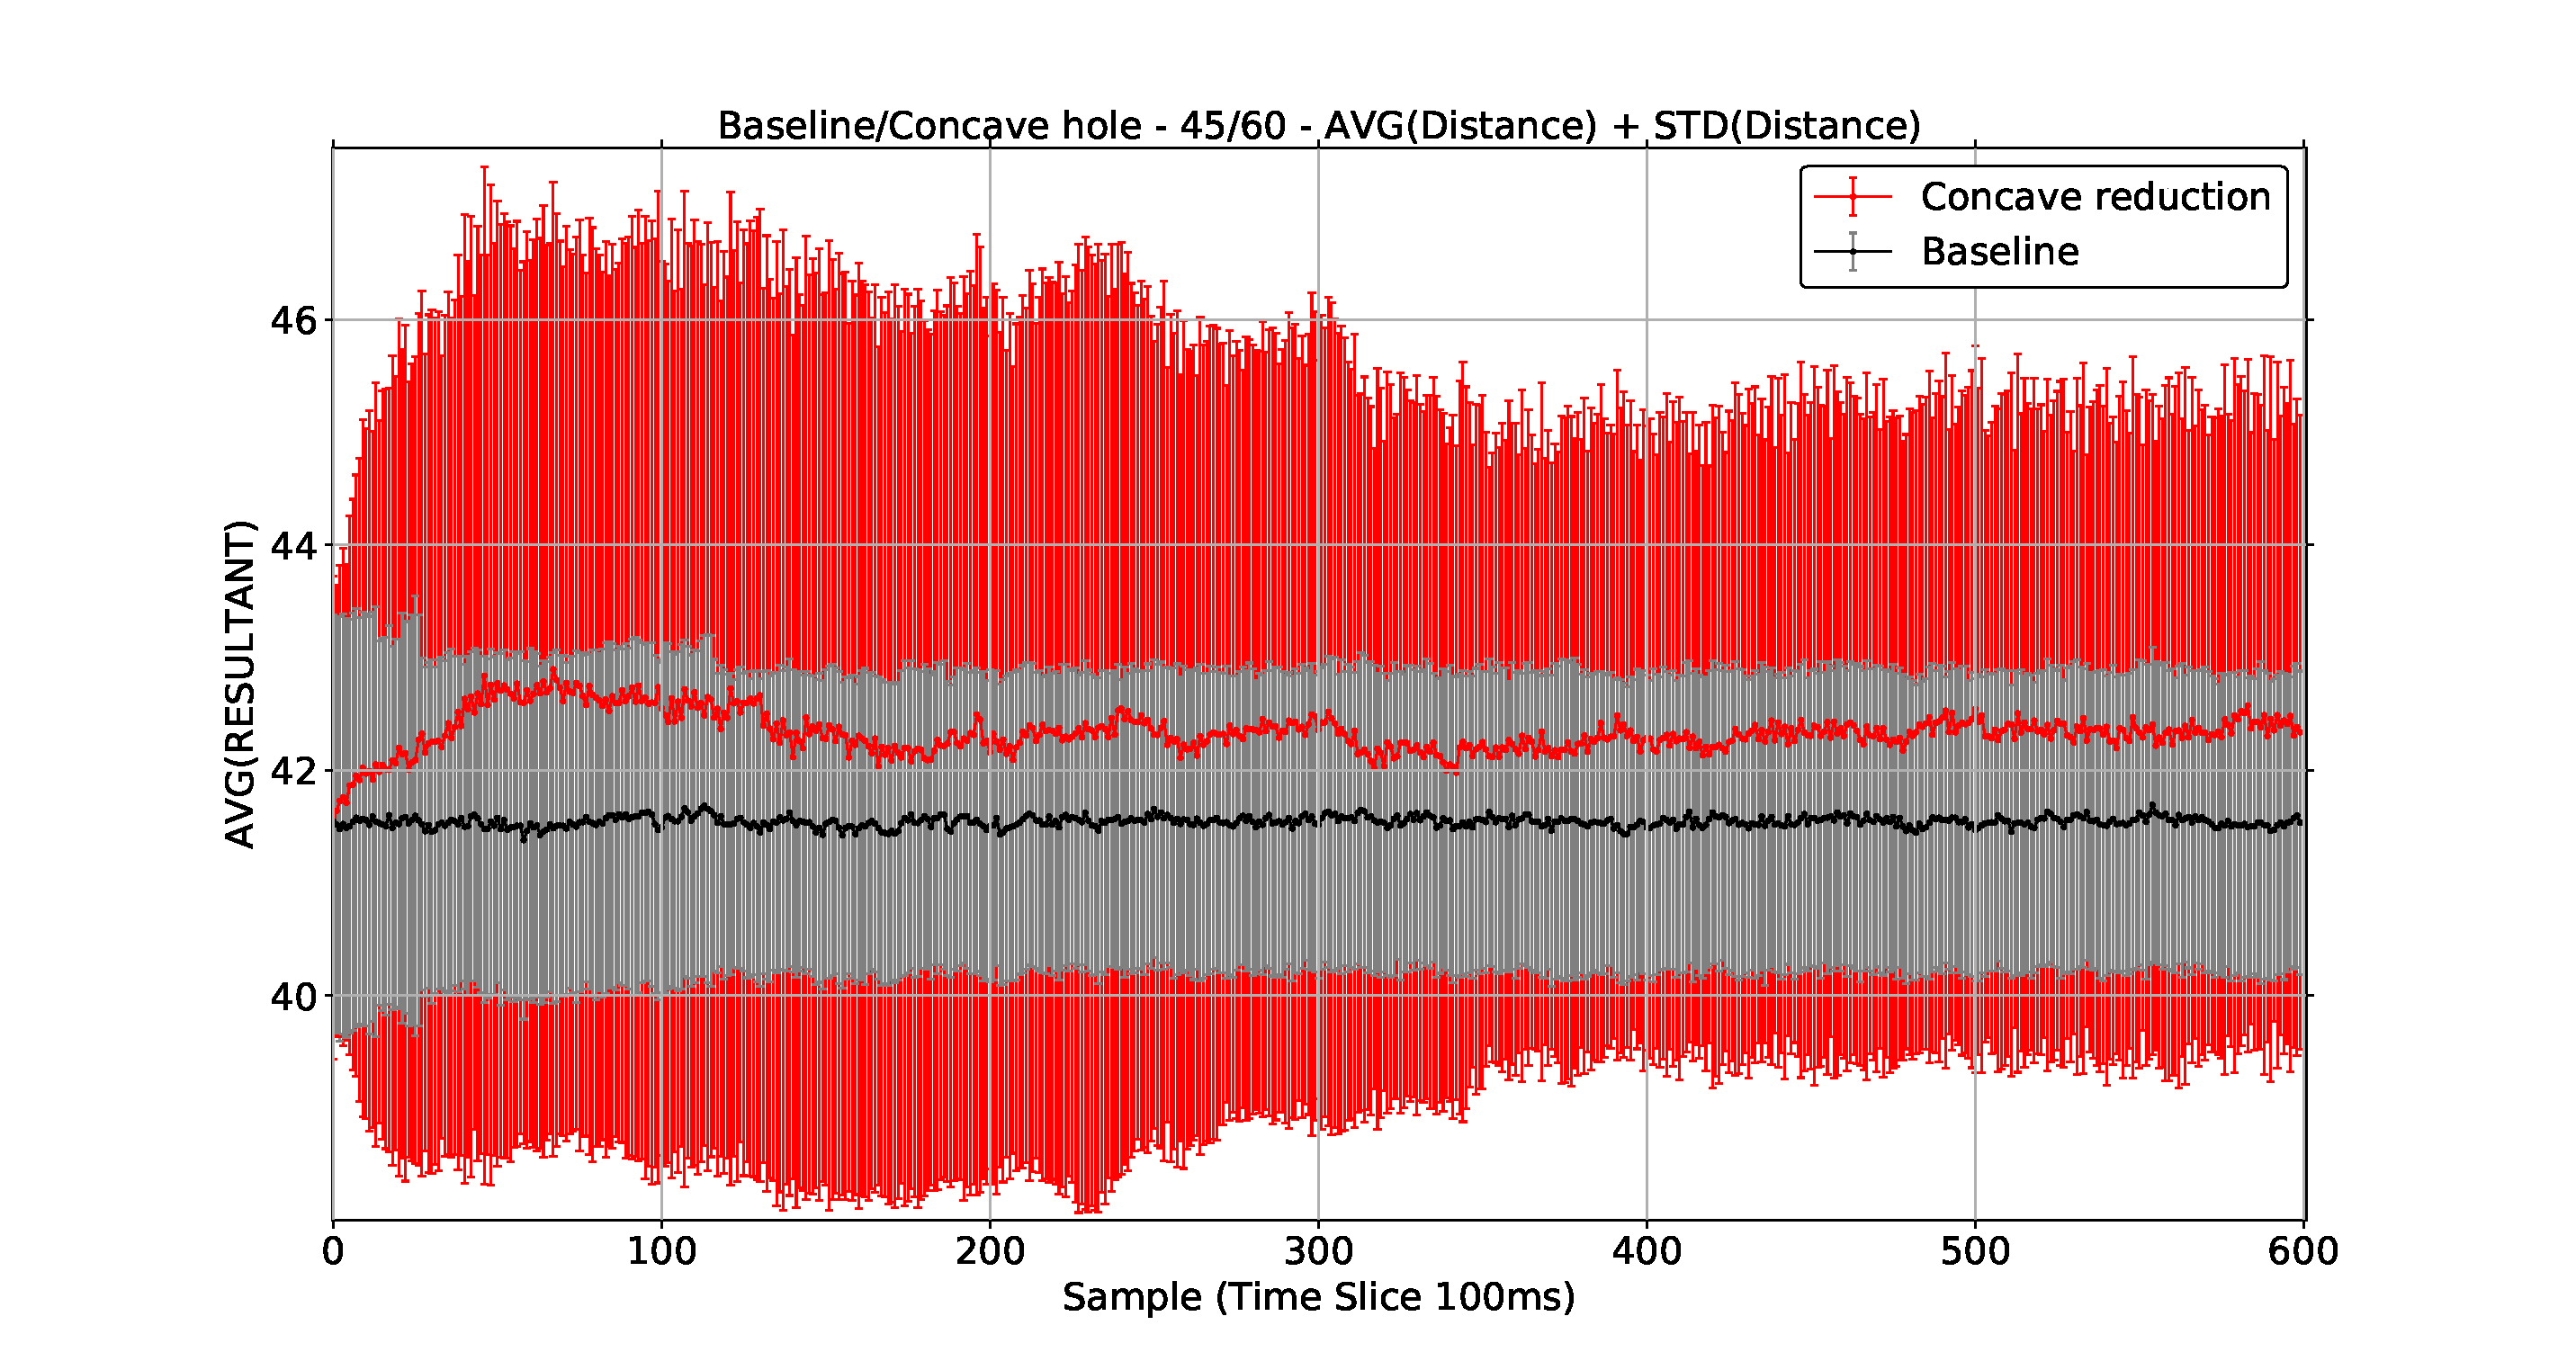
\includegraphics[width=15cm]{CHAPTER-7/figures/ConcavePerimeter4560-DIST}
\end{center}
\caption{Concave reduction stability effect distance\label{voids:ConcavePerimeter4560-DIST}}
\end{figure}

The residual jitter from 3.5 seconds on-wards~(Figire~\ref{voids:ConcavePerimeter4560-DIST-2}) is the algorithm's effect on the outer perimeter of the swarm. The baseline shows a steadier average with a reduced variance as the basic swarming algorithm allows the agents to settle to a formation that is more structurally stable.
%SWARMHOLE-DIST-4560.py
\begin{figure}[H]
\begin{center}
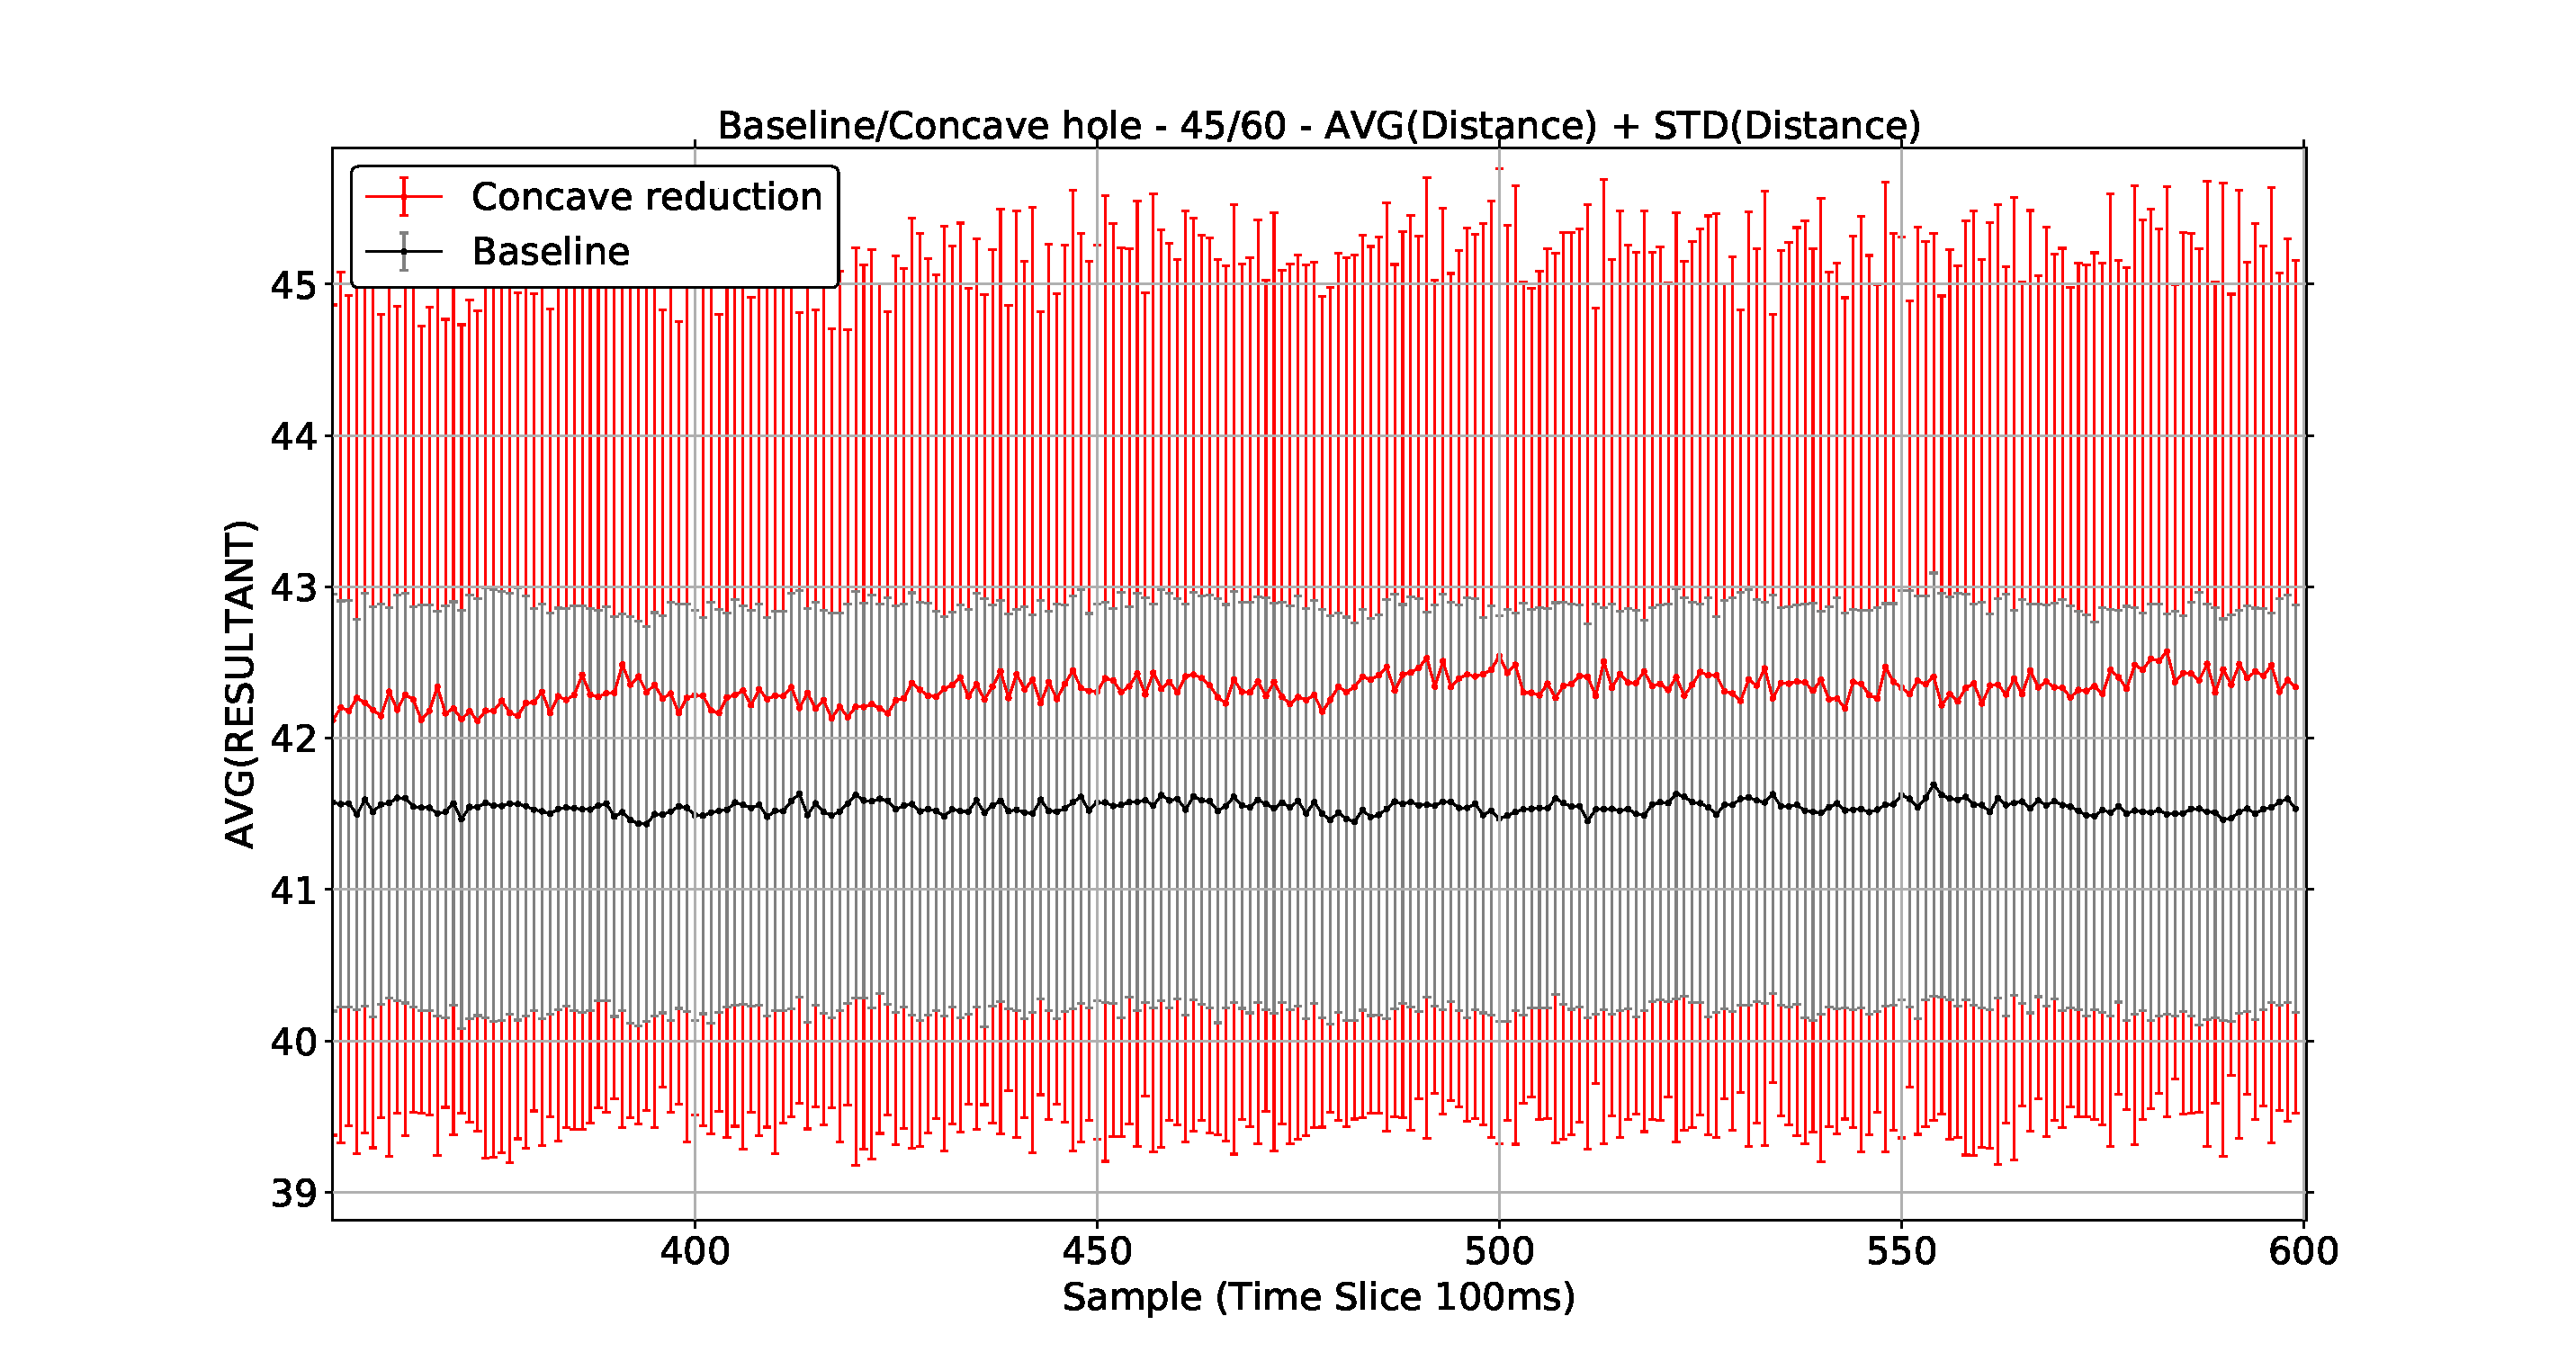
\includegraphics[width=15cm]{CHAPTER-7/figures/ConcavePerimeter4560-DIST-2}
\end{center}
\caption{Concave reduction stability effect distance\label{voids:ConcavePerimeter4560-DIST-2}}
\end{figure}

Figure~\ref{voids:ConcavePerimeter4560-MAG} shows that although the algorithm has introduced jitter and therefore increased both the average \textit{inter-agent magnitude} and the variance the resultant changes have not caused the swarm to become cohesively unstable. The magnitude and the variance never take the magnitude below 0. From 3.5 seconds the \textit{inter-agent magnitude} fluctuates slightly with an increased variance caused by the re-positioning of the `concave' agents. Although the agents are less structured the increased resultant magnitude ensures the swarm remains cohesive. 
%SWARMHOLE-MAG-4560.py
\begin{figure}[H]
\begin{center}
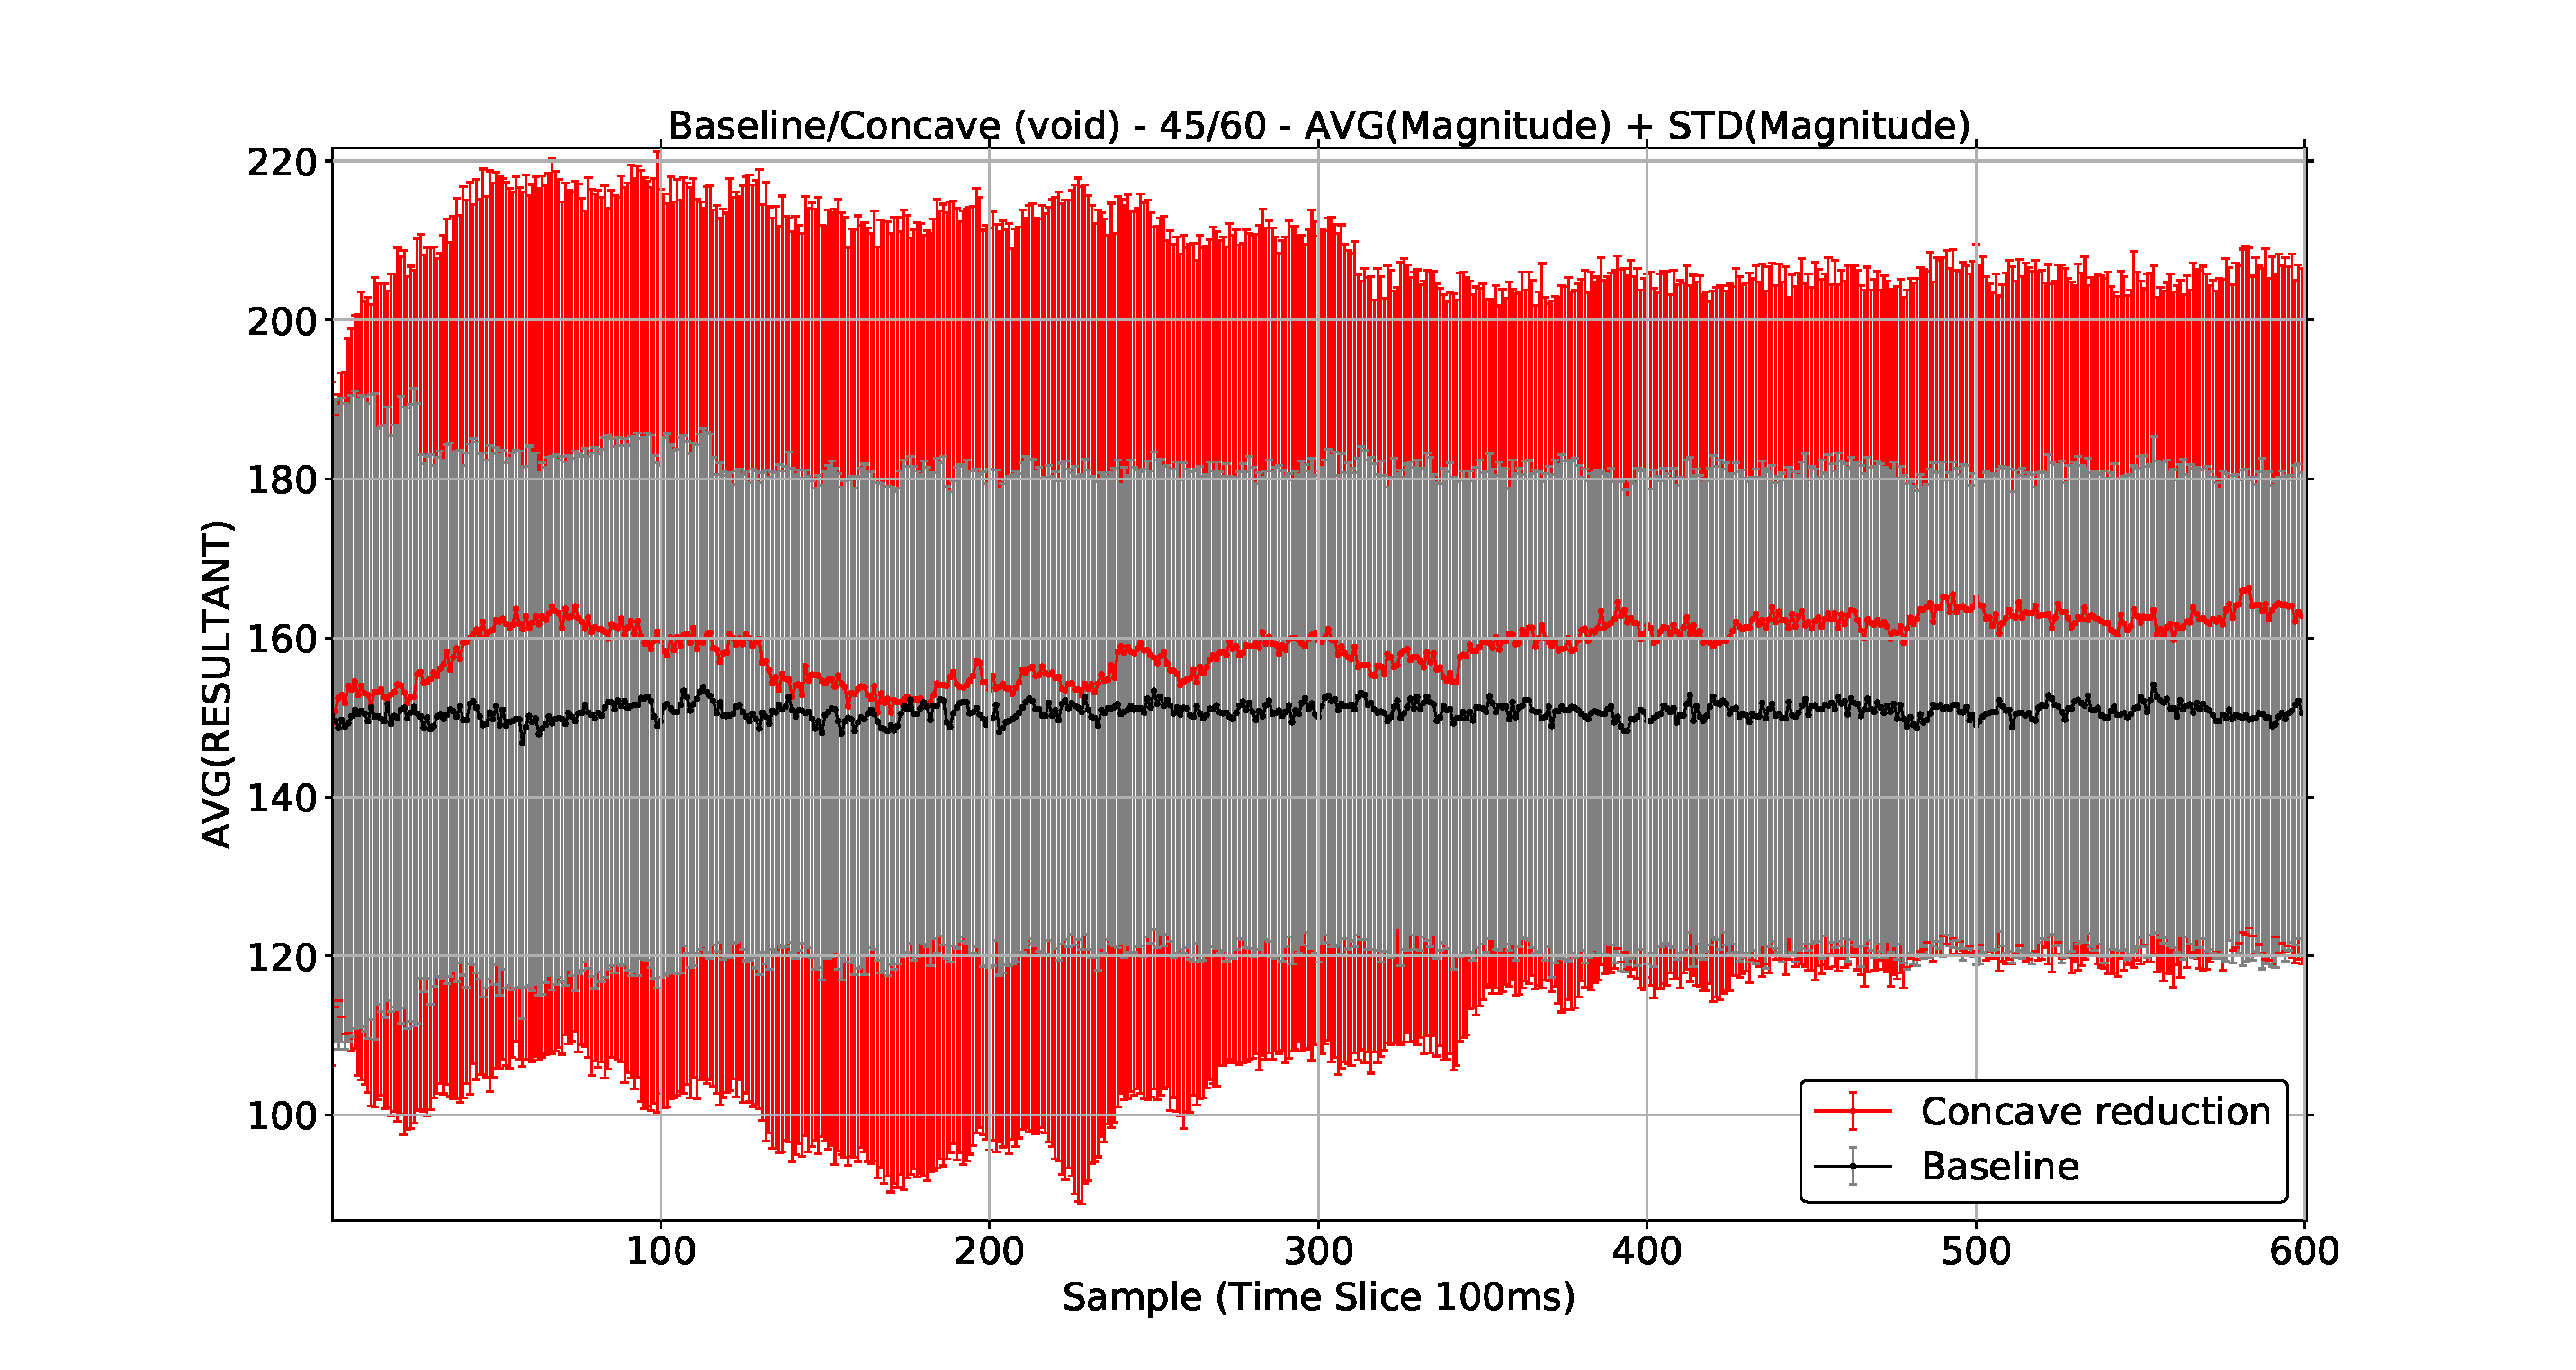
\includegraphics[width=15cm]{CHAPTER-7/figures/ConcavePerimeter4560-MAG}
\end{center}
\caption{Concave reduction stability effect magnitude\label{voids:ConcavePerimeter4560-MAG}}
\end{figure}

Once the void is removed the swarm settles to a more stable phase 3.5 seconds on-wards~(Figure~\ref{voids:ConcavePerimeter4560-MAG-2}), there is a slightly higher variance than the baseline which is caused by the concave reduction affected agents `pulling' the swarm. This `pulling' causes the agents to be slightly more distributed and therefore increases the inter-agent cohesion. There is also the addition of the `snapping' effect which increases the variance. 
%SWARMHOLE-MAG-4560.py
\begin{figure}[H]
\begin{center}
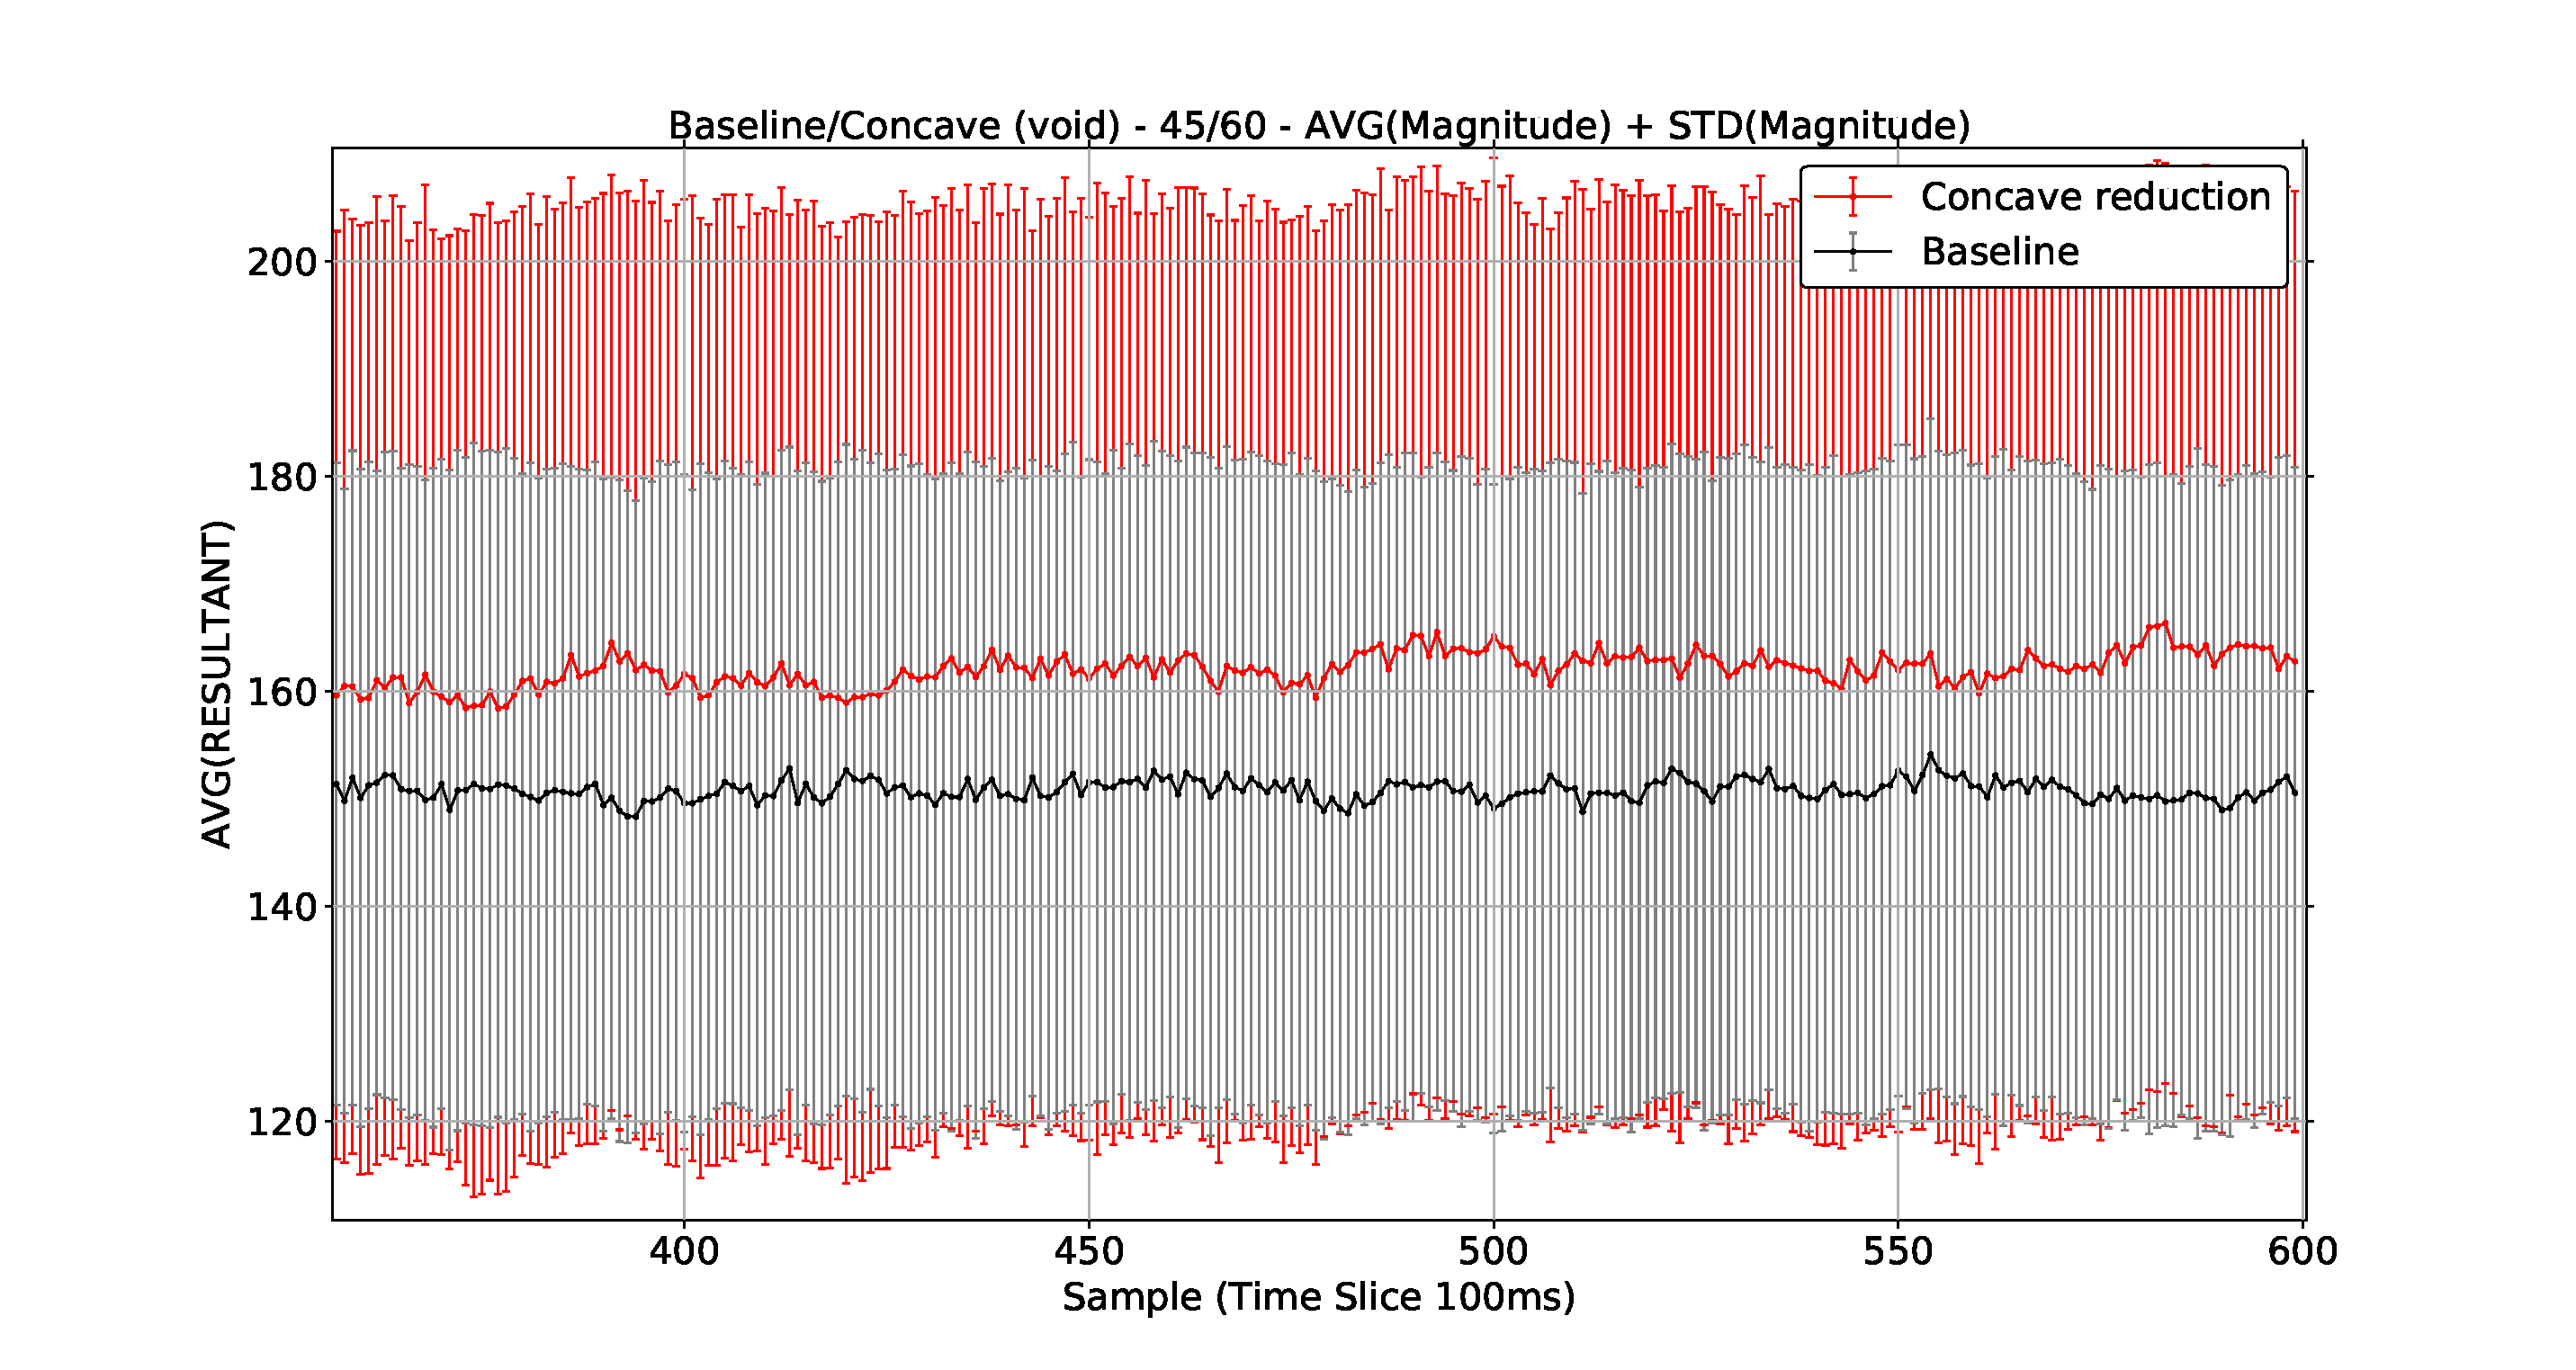
\includegraphics[width=15cm]{CHAPTER-7/figures/ConcavePerimeter4560-MAG-2}
\end{center}
\caption{Concave reduction stability effect magnitude\label{voids:ConcavePerimeter4560-MAG-2}}
\end{figure}

The effect on the swarm of removing the void is to reduce the overall number of perimeter agents. Figure~\ref{methods:ConcavePerimeter4560-1} shows that as the void is removed from the swarm the number of perimeter agents falls. The change in size is caused by two processes. The swarm structure is being altered on the outer perimeter as the agents move towards a more circular formation and the internal agents identified as perimeter agents of a void move to reduce the internal anomaly. 

Once the initial disorganised phase settles, which takes approximately 1.2 seconds, the effect of the concave reduction starts to take effect. The perimeter size starts to reduce. The majority of the reduction is the void shrinking. The swarm then goes through a settling period where the overall perimeter size of the swarm stabalises and eventually the residual snapping effect is left at the outer perimeter. This occurs at approximately 3.5 seconds into the simulation. 
%PERIMETER4560HOLE.py
\begin{figure}[H]
\begin{center}
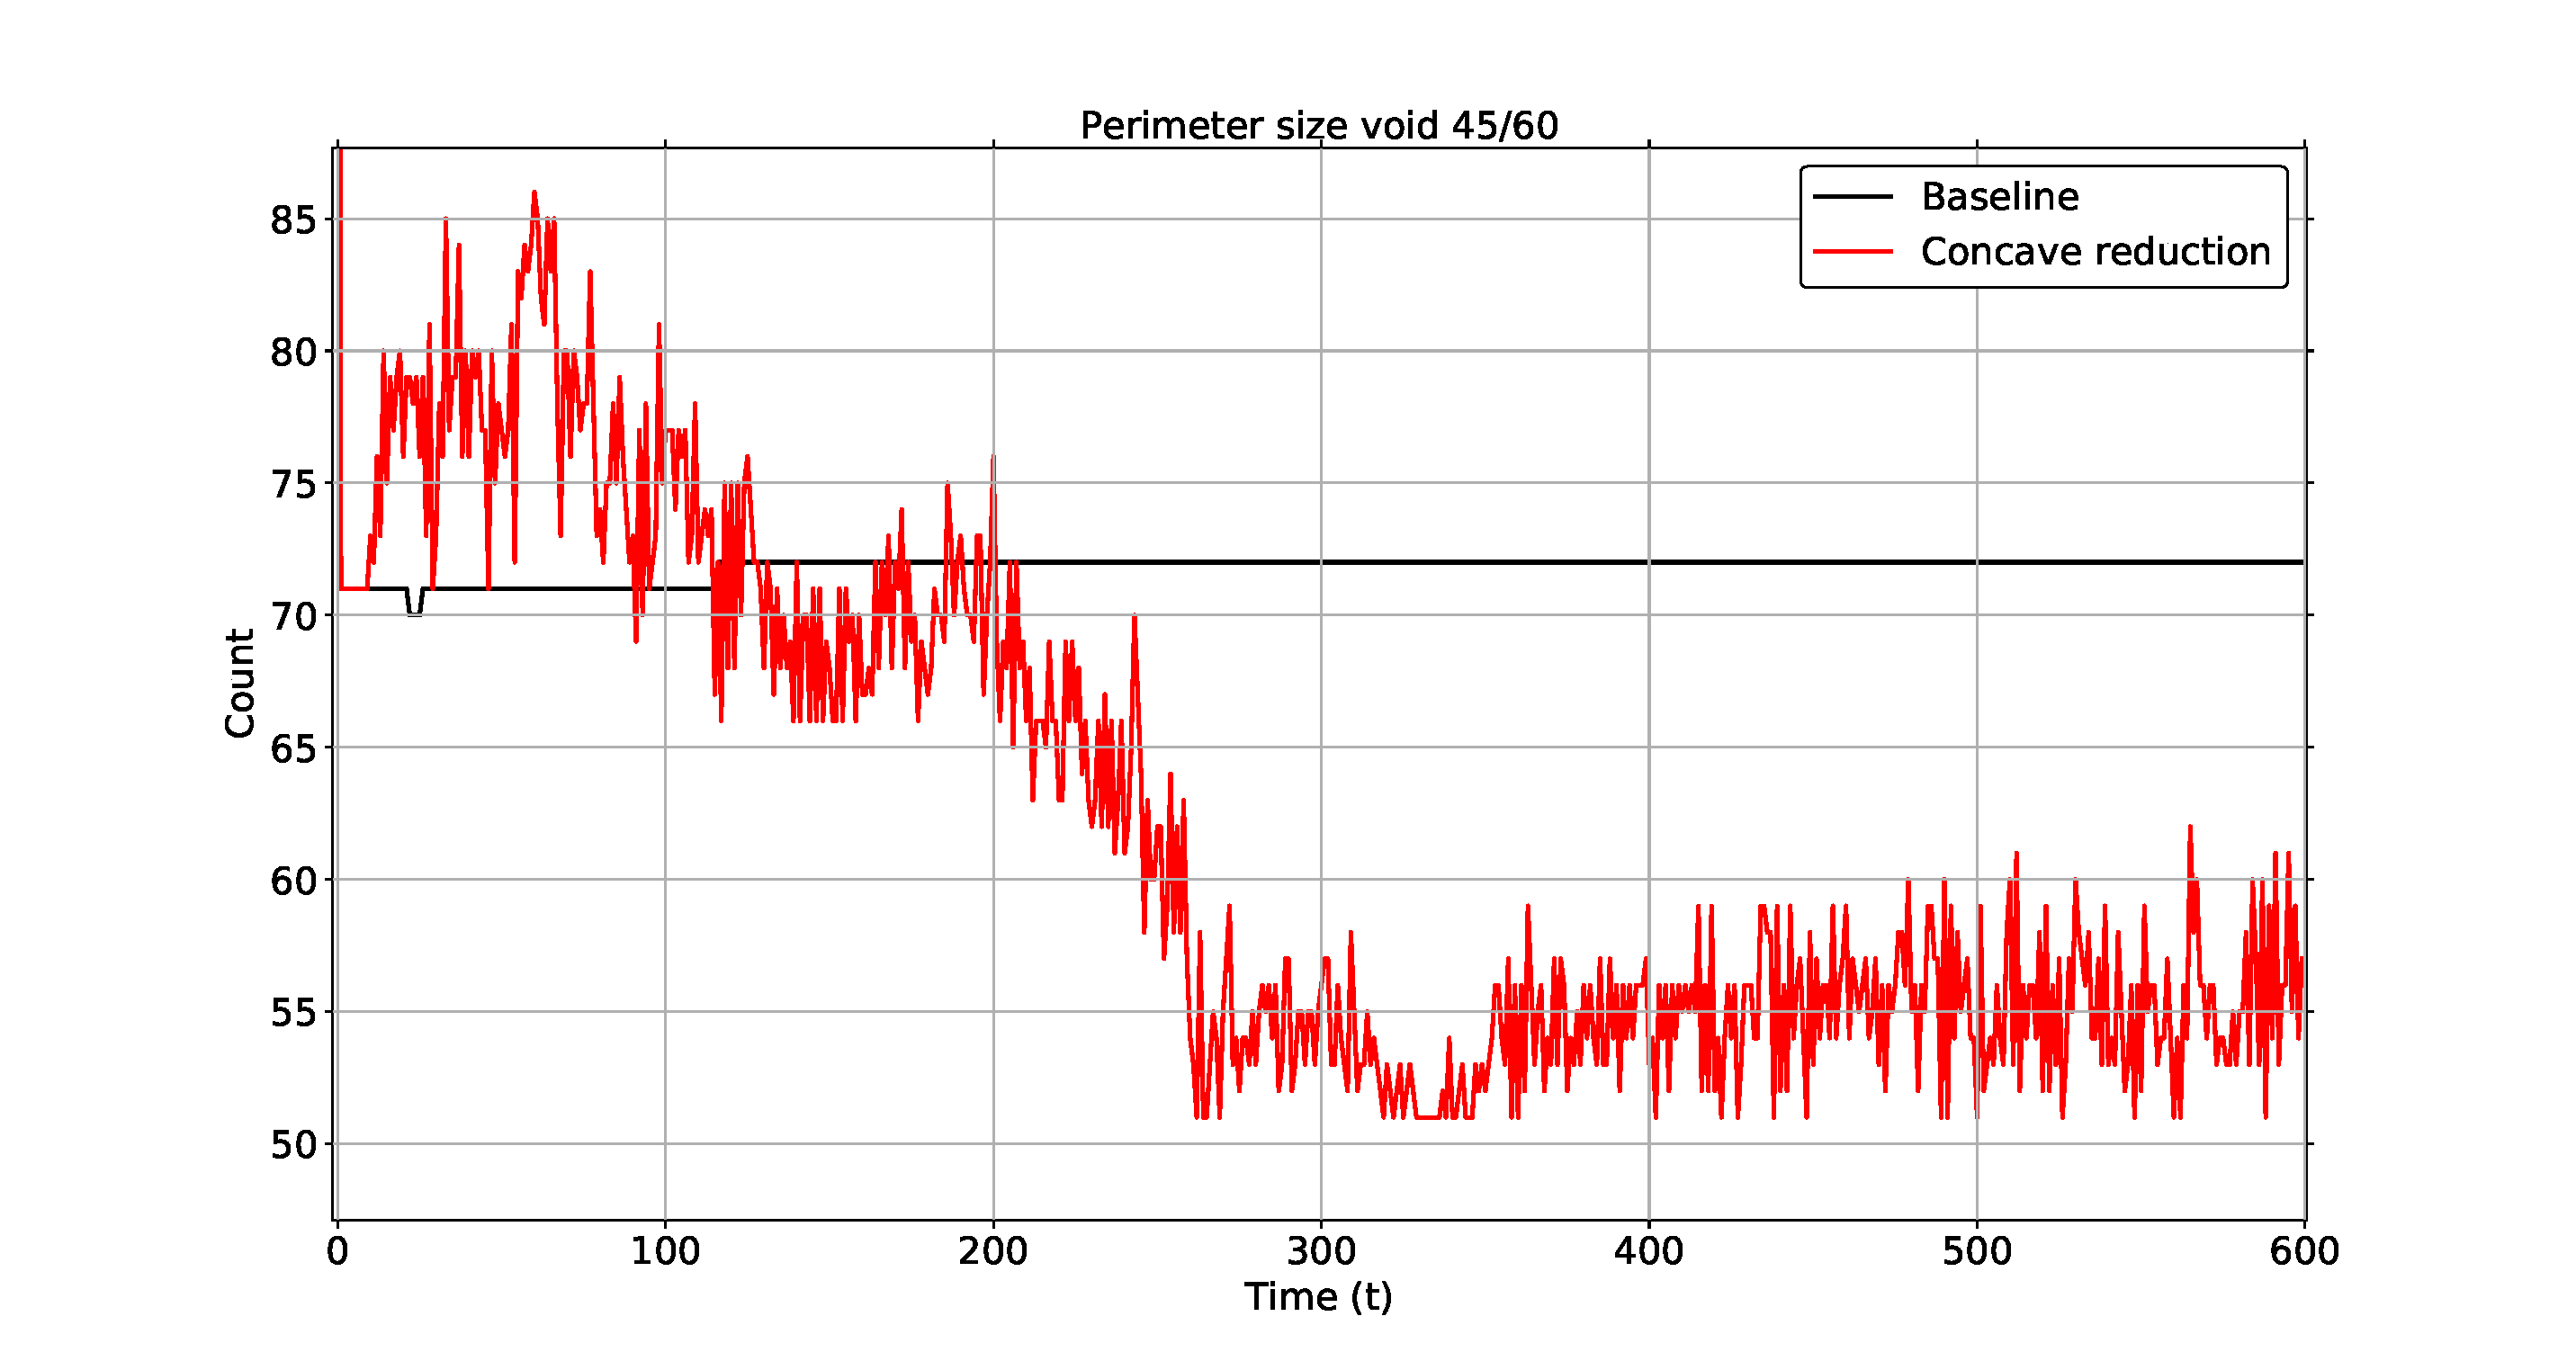
\includegraphics[width=15cm]{CHAPTER-7/figures/ConcavePerimeter4560-1}
\end{center}
\caption{Concave reduction perimeter effect\label{methods:ConcavePerimeter4560-1}}
\end{figure}

The effect on the swarm's structure is shown in Figures~\ref{voids:SwarmCoverage4560-1} and~\ref{voids:SwarmCoverage4560-2}. Figure~\ref{voids:SwarmCoverage4560-1} shows the agents positions during the simulation for the baseline and the concave reduction enabled swarms. The baseline swarm is shown in black. The red traces are for the swarm using concave reduction. Figure~\ref{voids:SwarmCoverage4560-2} is a more detailed view highlighting the baseline lattice structure.
%COVERBASELINE4560.py
\begin{figure}[H]
\begin{center}
\includegraphics[width=15cm]{CHAPTER-7/figures/SwarmCoverage4560-1}
\end{center}
\caption{Agent movement comparison\label{voids:SwarmCoverage4560-1}}
\end{figure}

The overall effect of the concave reduction on the swarm's movement can be seen in~figure~\ref{voids:SwarmCoverage4560-1}. The void is closed by the reduction and the overall area of the swarm is reduced. There is however a negative effect with respect to the concave reduction; the swarm has a directional bias due to the large straight edge which causes the swarm to `drift'. When looking closely at the positions (Figure~\ref{voids:SwarmCoverage4560-2}) the baseline agents remain relatively static in their positions vibrating slightly to maintain the equilibrium of the internal magnitudes. 
%COVERBASELINE4560.py
\begin{figure}[H]
\begin{center}
\includegraphics[width=15cm]{CHAPTER-7/figures/SwarmCoverage4560-2}
\end{center}
\caption{Agent movement comparison\label{voids:SwarmCoverage4560-2}}
\end{figure}

\section{Concave reduction for object surrounding}\label{voids:ObjectSurrounding}
Concave reduction has the benefit of creating a convex-perimeter and removing a concave perimeter. This effect can be applied to surrounding objects. As a void is removed agents still avoid obstacles, this results in a perimeter edge that tightly encloses an object's perimeter. The concept of detecting an object and surrounding it is not new. In 2013 Zhang et al~\cite{ZFG:13} investigated this as a mechanism to assist in oil spillage containment. The process they used was based on ant-colony foraging. The agents initially carried out reconnaissance to detect a spillage, once a target is identified the agents use a communications infrastructure to inform nearby agents of the location of the spillage and the agents then use a \textit{destination vector} to locate the spill. To surround the spill the agents move in an anti-clockwise manner following the perimeter wall of the target. This thesis uses a different approach to solve this same problem.

One problem with the above approach is that the swarm may not find the spillage due to the paths the agents take when foraging not intersecting with the spillage. Another problem is that the system does not consider multiple targets. Finally there is the issue of the swarm requiring a communications infrastructure. 

This thesis focuses on arbitrary sized, low cost, swarms; this is a similar approach to the US Navy in the LOCUST project~\cite{MW:15, DS:15}. Also the approach of using concave reduction removes the need for a communications infrastructure. 

Consider an oil slick in an environment. This could be a section of open-water or a lake/reservoir. The solution is to deploy a swarm at the perimeter of the known area by a boat or at a shoreline if the area is small enough~(Figure~\ref{voids:OilSlick}). The deployed agents, using local sensing and the concave reduction algorithm, are enabled. The swarm initially expands to an optimum distribution for the specified field effects. The \textit{concavity reduction vector} will then reduce the deliberately created void and the swarm encapsulates the oil spill. If there are multiple spills within the area the void reduction process will still encapsulate the area because the algorithm is not dependant on communications and operates purely by logic.  

\begin{figure}[H]
\begin{center}
\includegraphics[width=12cm]{CHAPTER-7/figures/OilSlick}
\end{center}
\caption{Concave reduction oil slick surrounding\label{voids:OilSlick}}
\end{figure}

Figure~\ref{concave:OilSpillSimulation} is a screen shot of the deployment within the simulator for testing this hypothesis. 

\begin{figure}[H]
\begin{center}
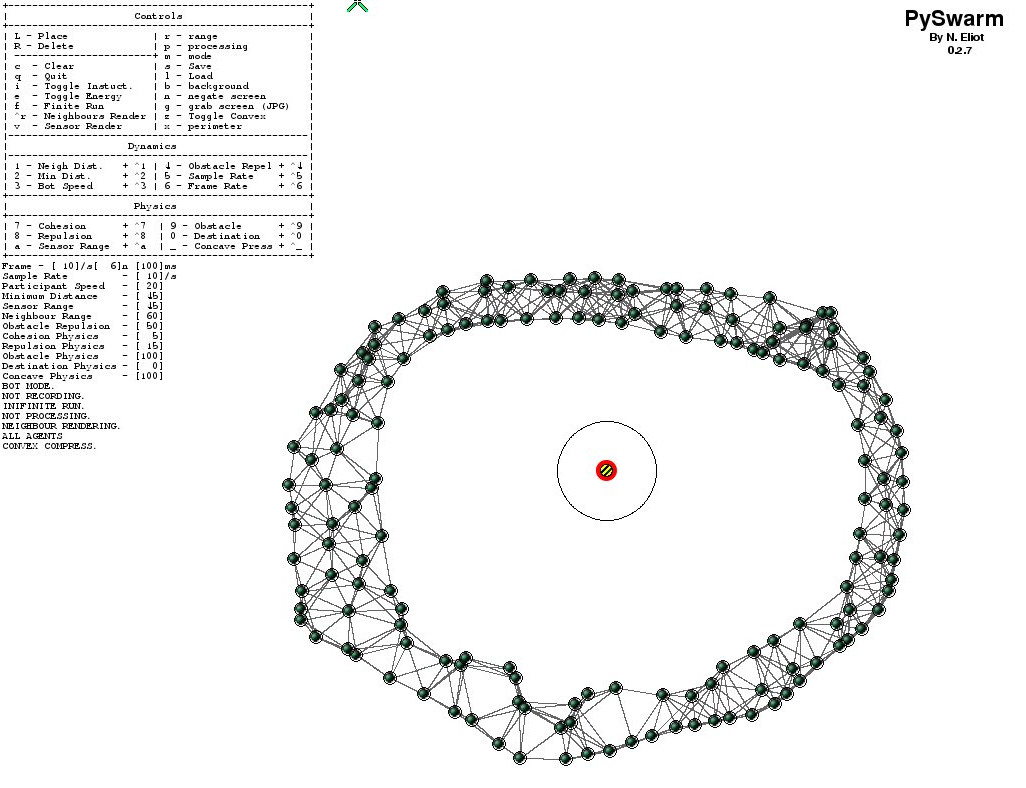
\includegraphics[width=14cm]{CHAPTER-7/figures/OilSpillSimulator}
\end{center}
\caption{Oil spill containment simulation\label{concave:OilSpillSimulation}}
\end{figure}

Figure~\ref{fig:OilSpillConcaveReduction1} shows the containment process using the baseline configuration without concave reduction. The swarm expands due to the field effects and then stabilises into a swarm which contains a void area. The swarm stablises and the swarm moves slightly as the cohesion and repulsion fluctuate to maintain the swarm's structure. However the void does not close and the containment process does not occur. The agents that do come in contact with the obstacle are repelled by the obstacle repulsion field.

\begin{figure}[H]
\centering
\subfigure[Initial]{
    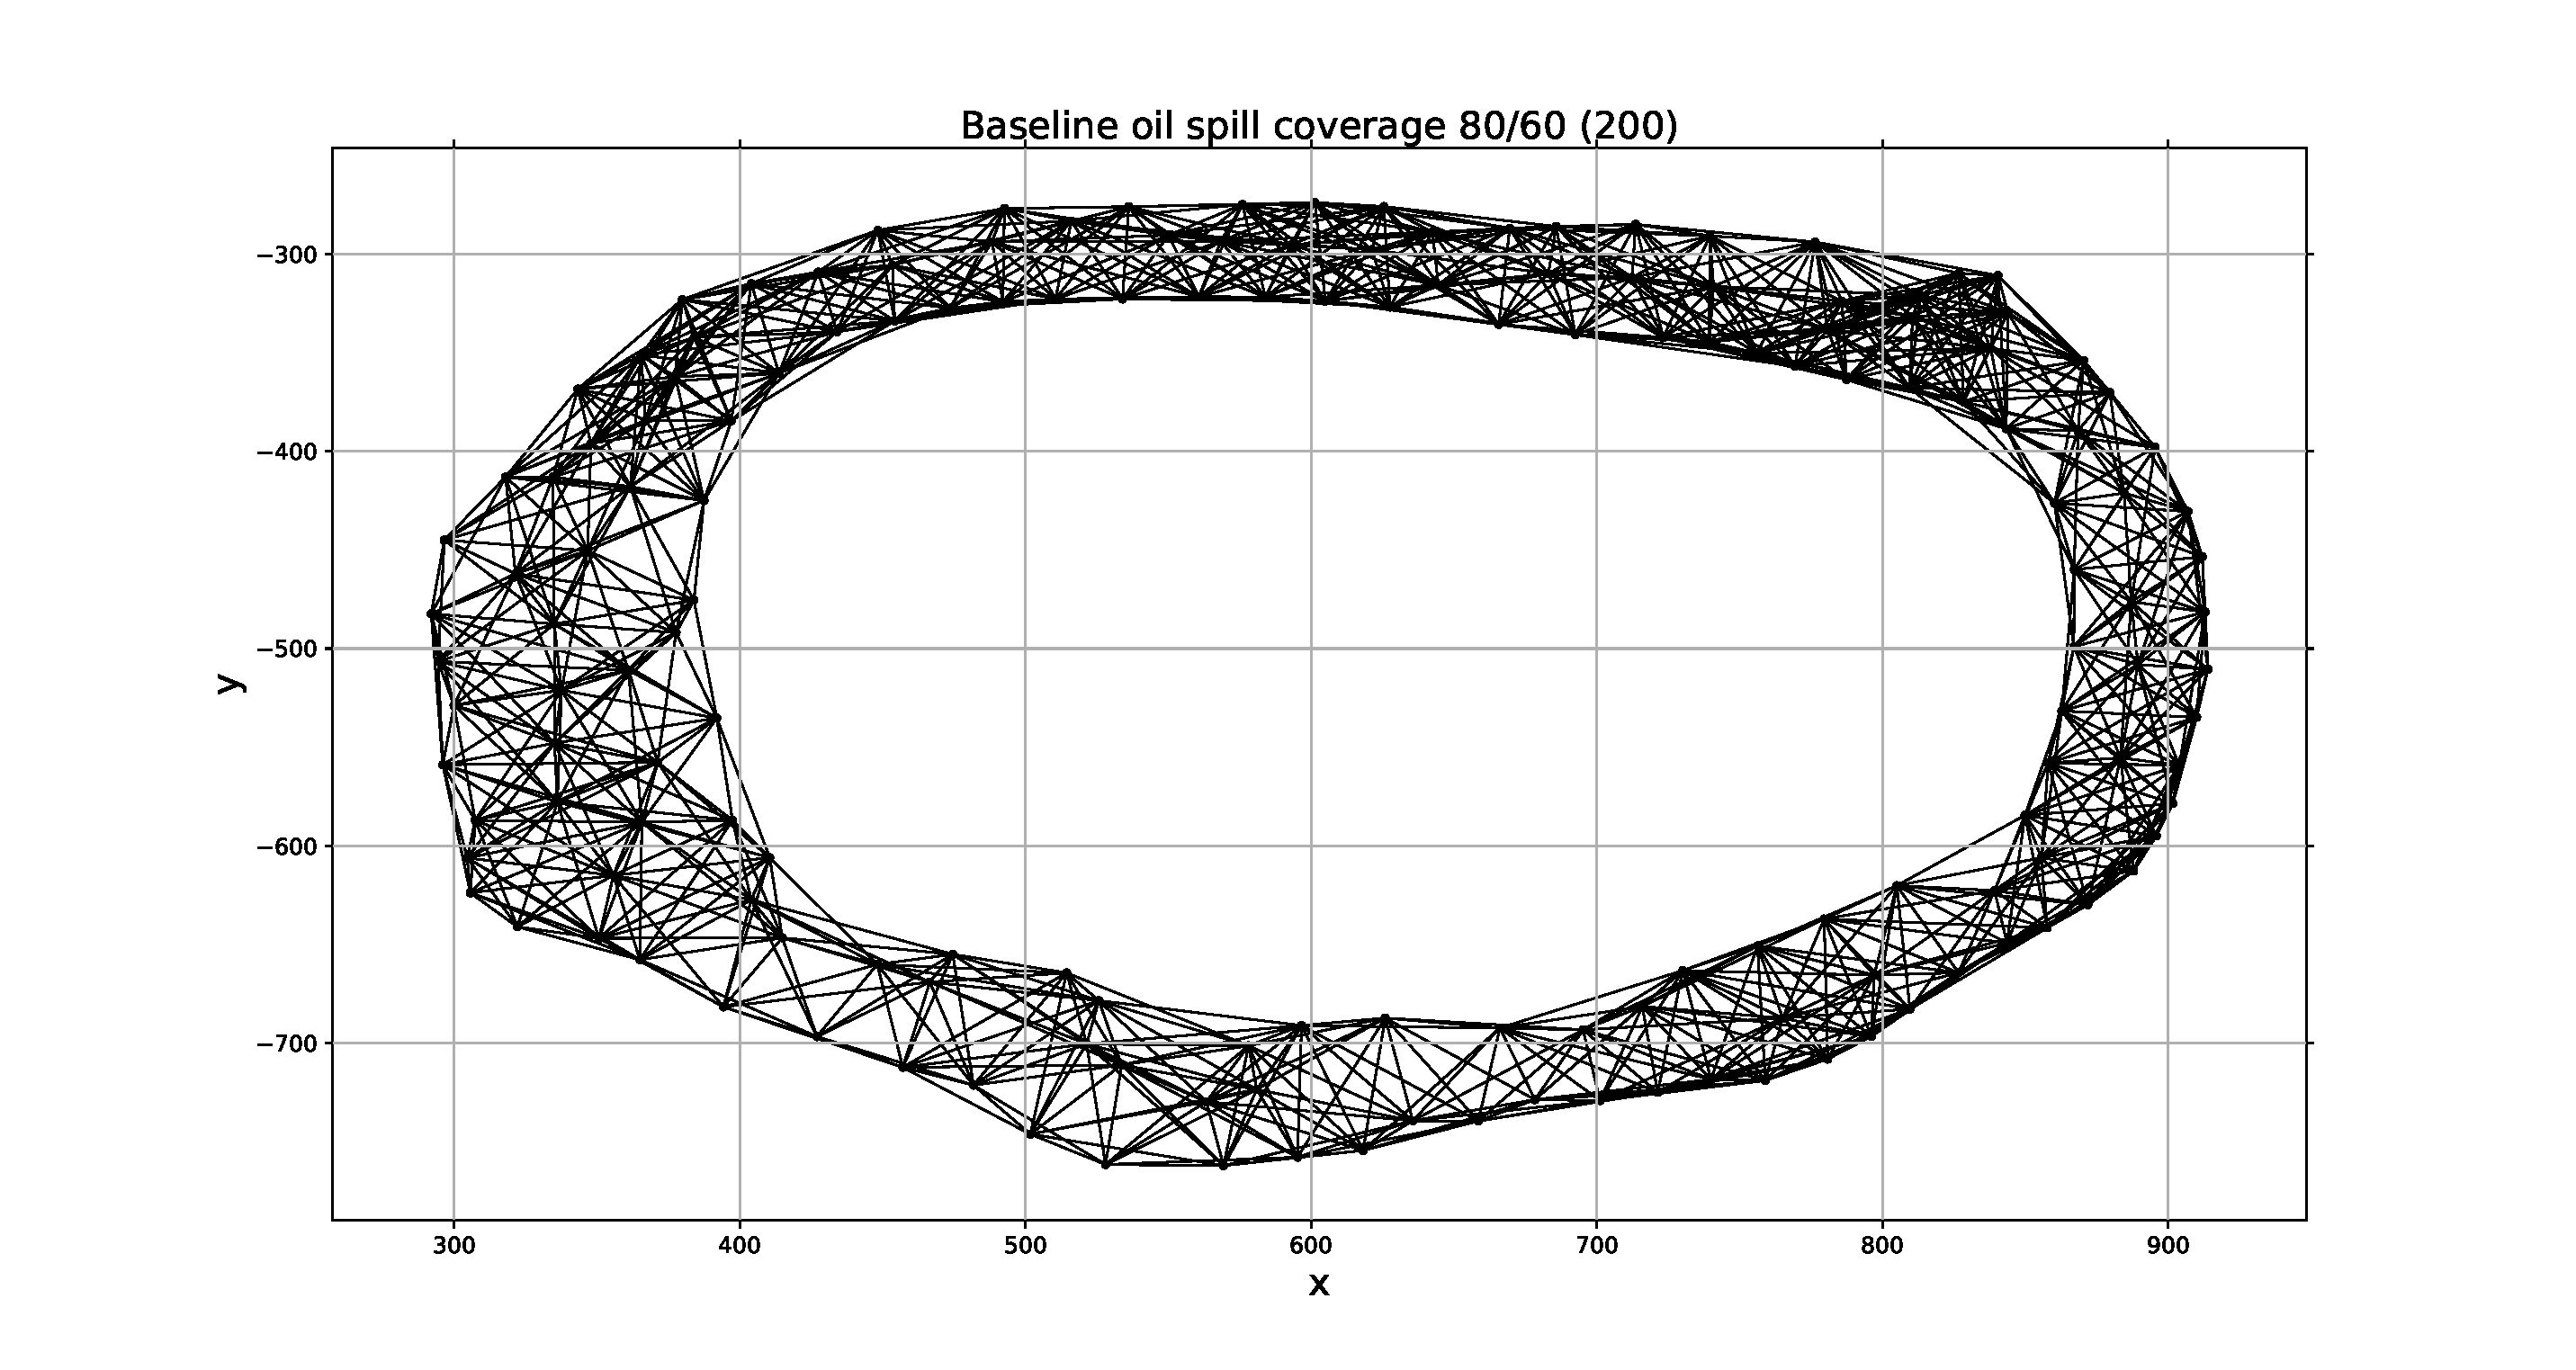
\includegraphics[width=6cm]{CHAPTER-7/figures/OilSpillBase1}
    \label{concave:OilSpillBase1}
}
\subfigure[Partial]{
    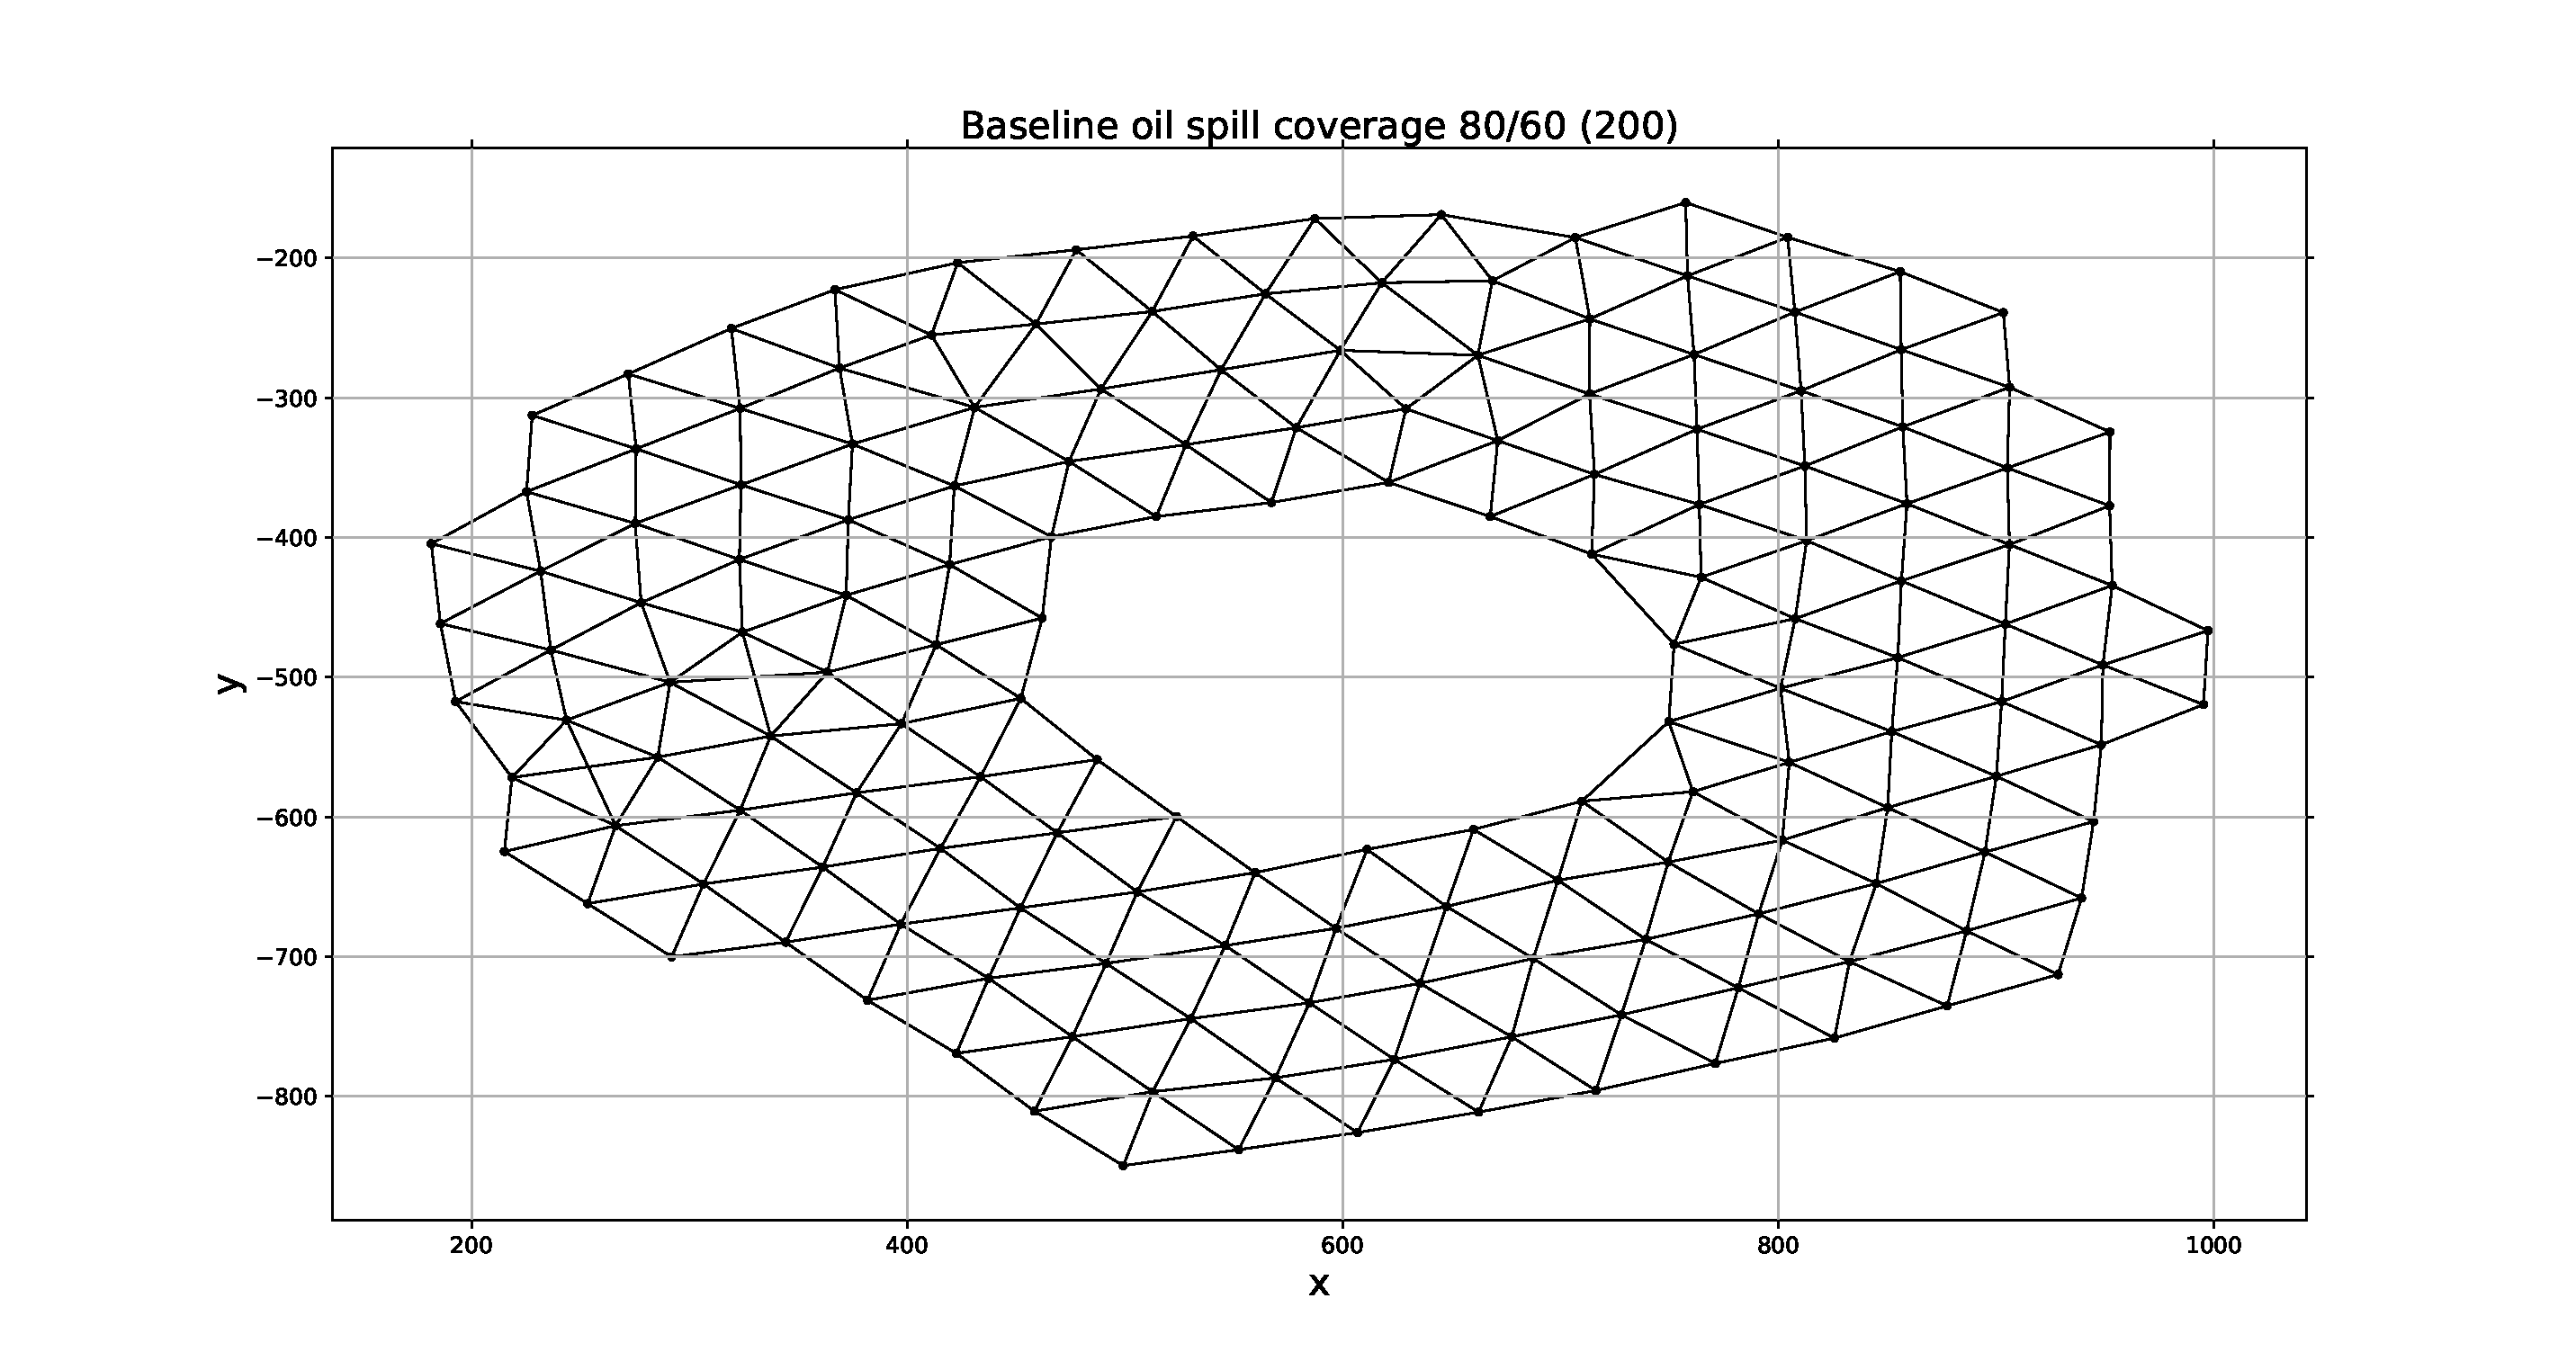
\includegraphics[width=6cm]{CHAPTER-7/figures/OilSpillBase2}
    \label{fig:OilSpillBase2}
}
\subfigure[End]{
    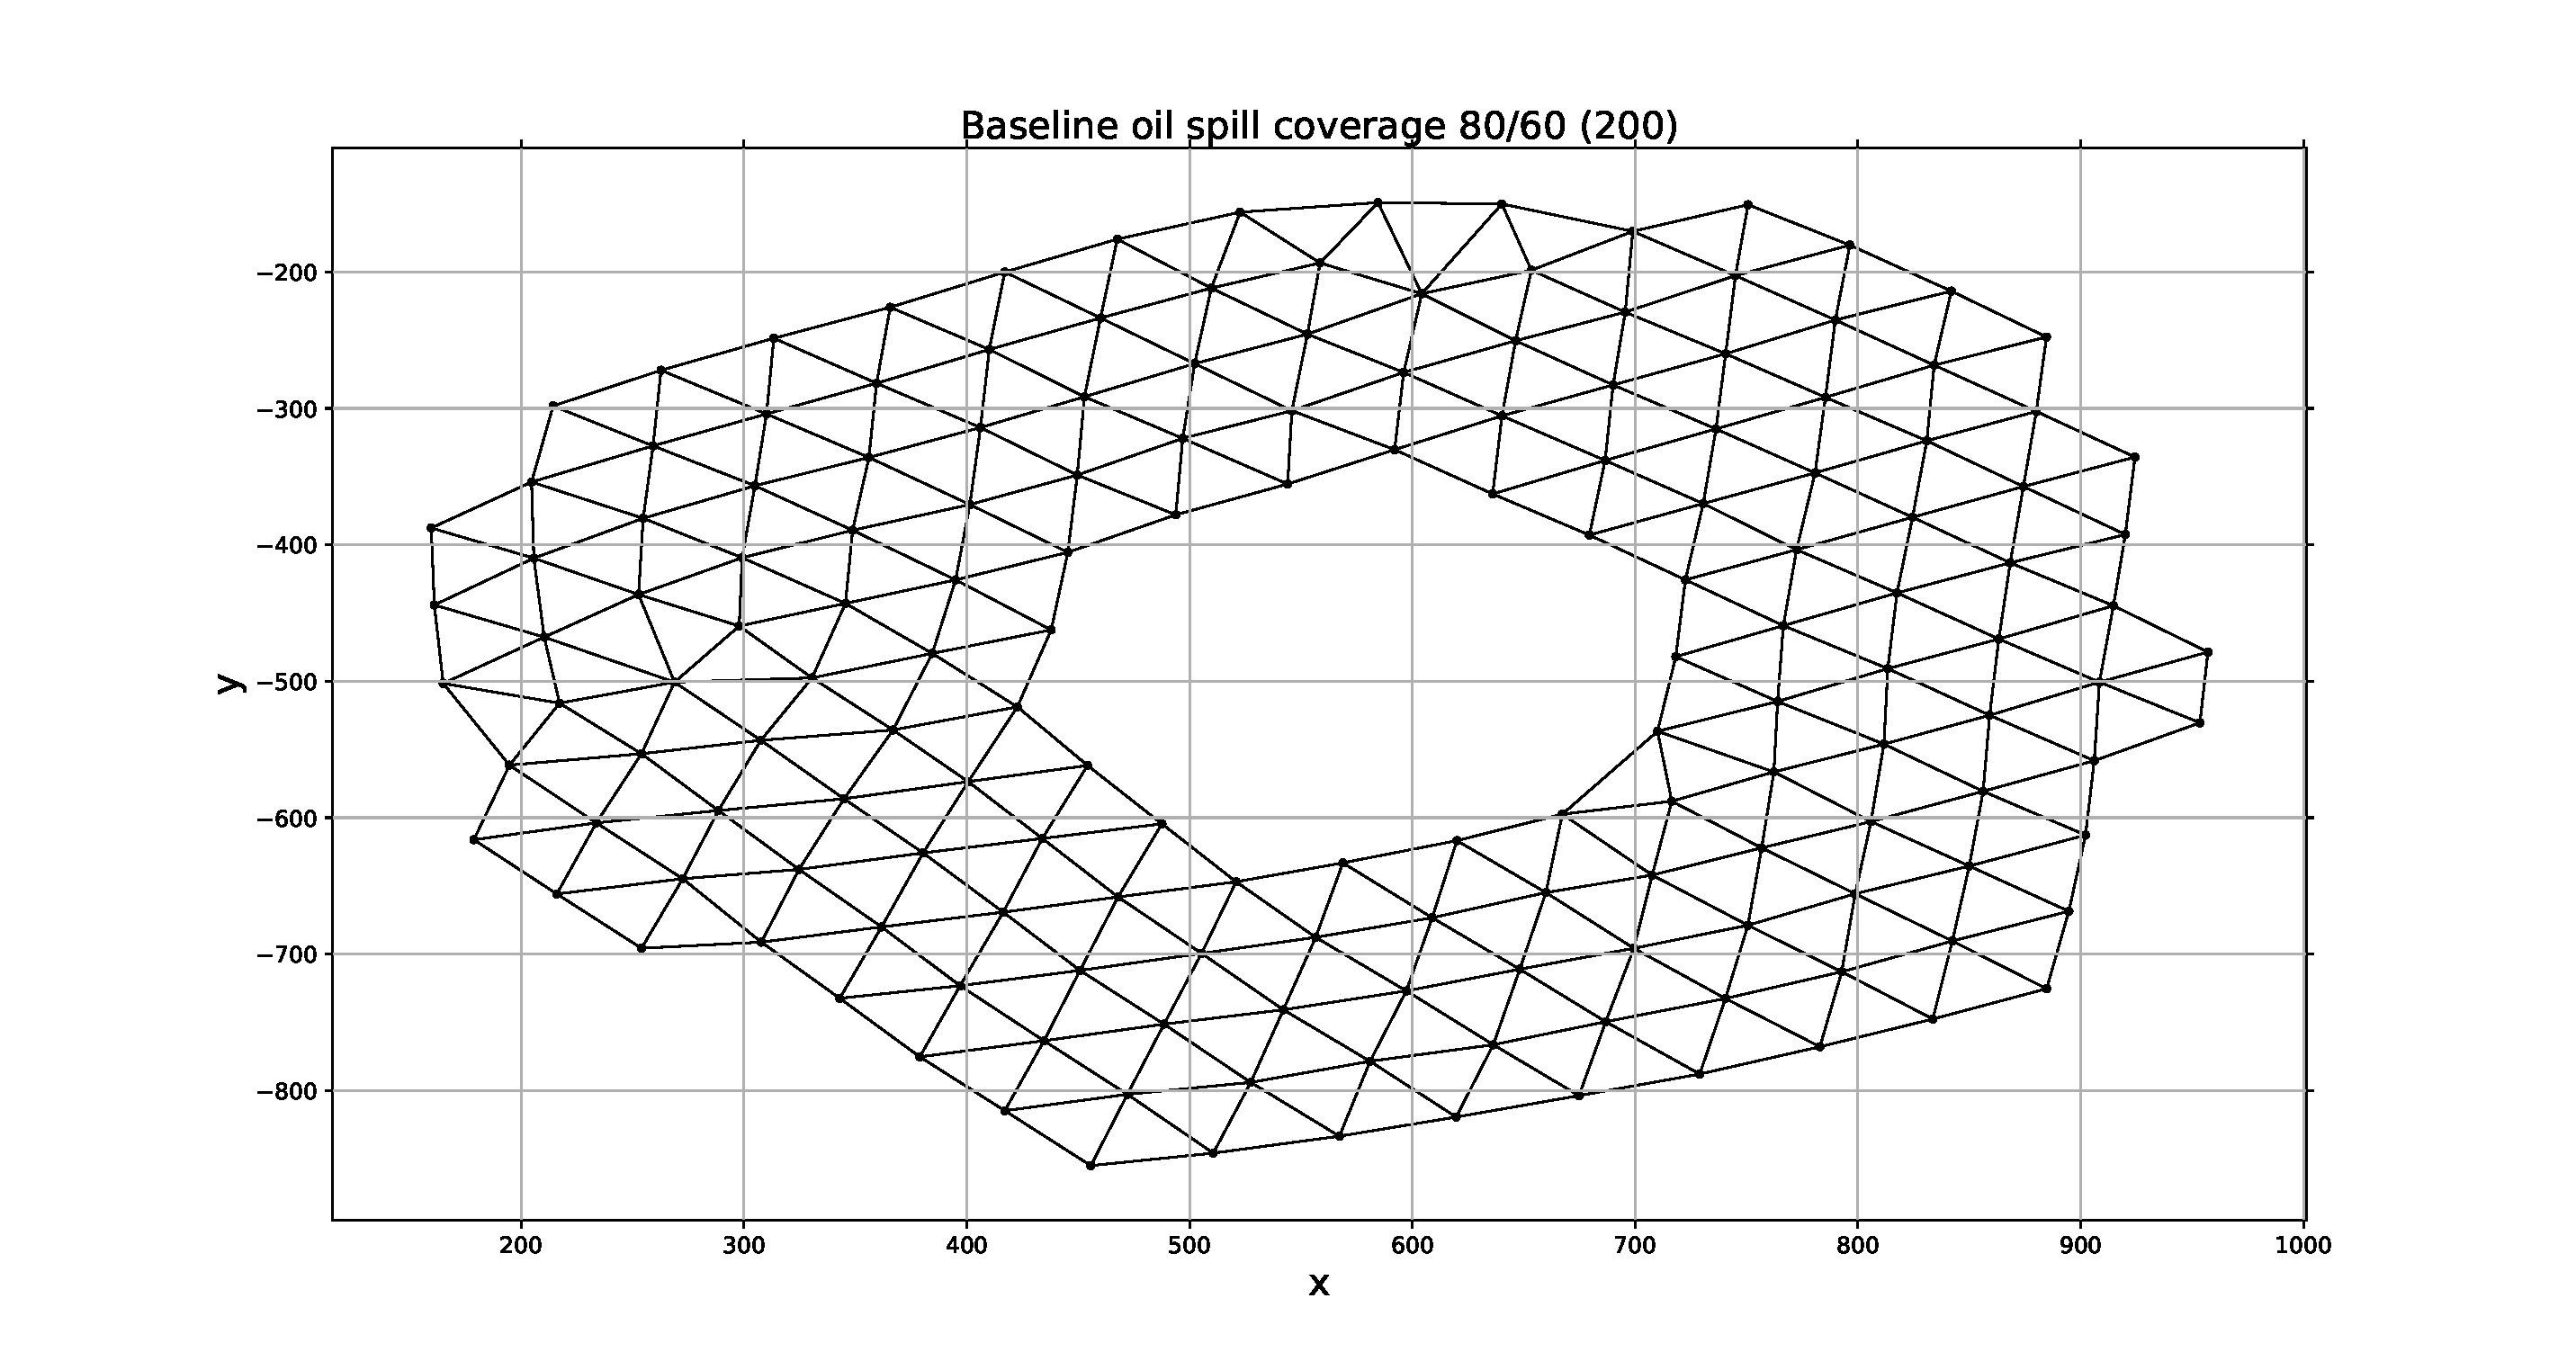
\includegraphics[width=6cm]{CHAPTER-7/figures/OilSpillBase3}
    \label{fig:OilSpillBase3}
}
\caption{Baseline oil spill containment}
\label{fig:OilSpillConcaveReduction1}
\end{figure}

Figure~\ref{fig:VoidConcaveReduction} shows the same simulation with void-reduction activated. The swarm expands as expected due to the field effects but in addition the concave reduction reduces the void within the swarm. This reduction in the void causes the swarm to shrink around the obstacle completely enclosing it at the obstacle perimeter. On the left hand side of~figure~\ref{fig:OilSpillConcave2} the percolation effect can be seen as described in~section~\ref{sec:ApplicationConcavePerimeters}.

\begin{figure}[H]
\centering
\subfigure[Initial]{
    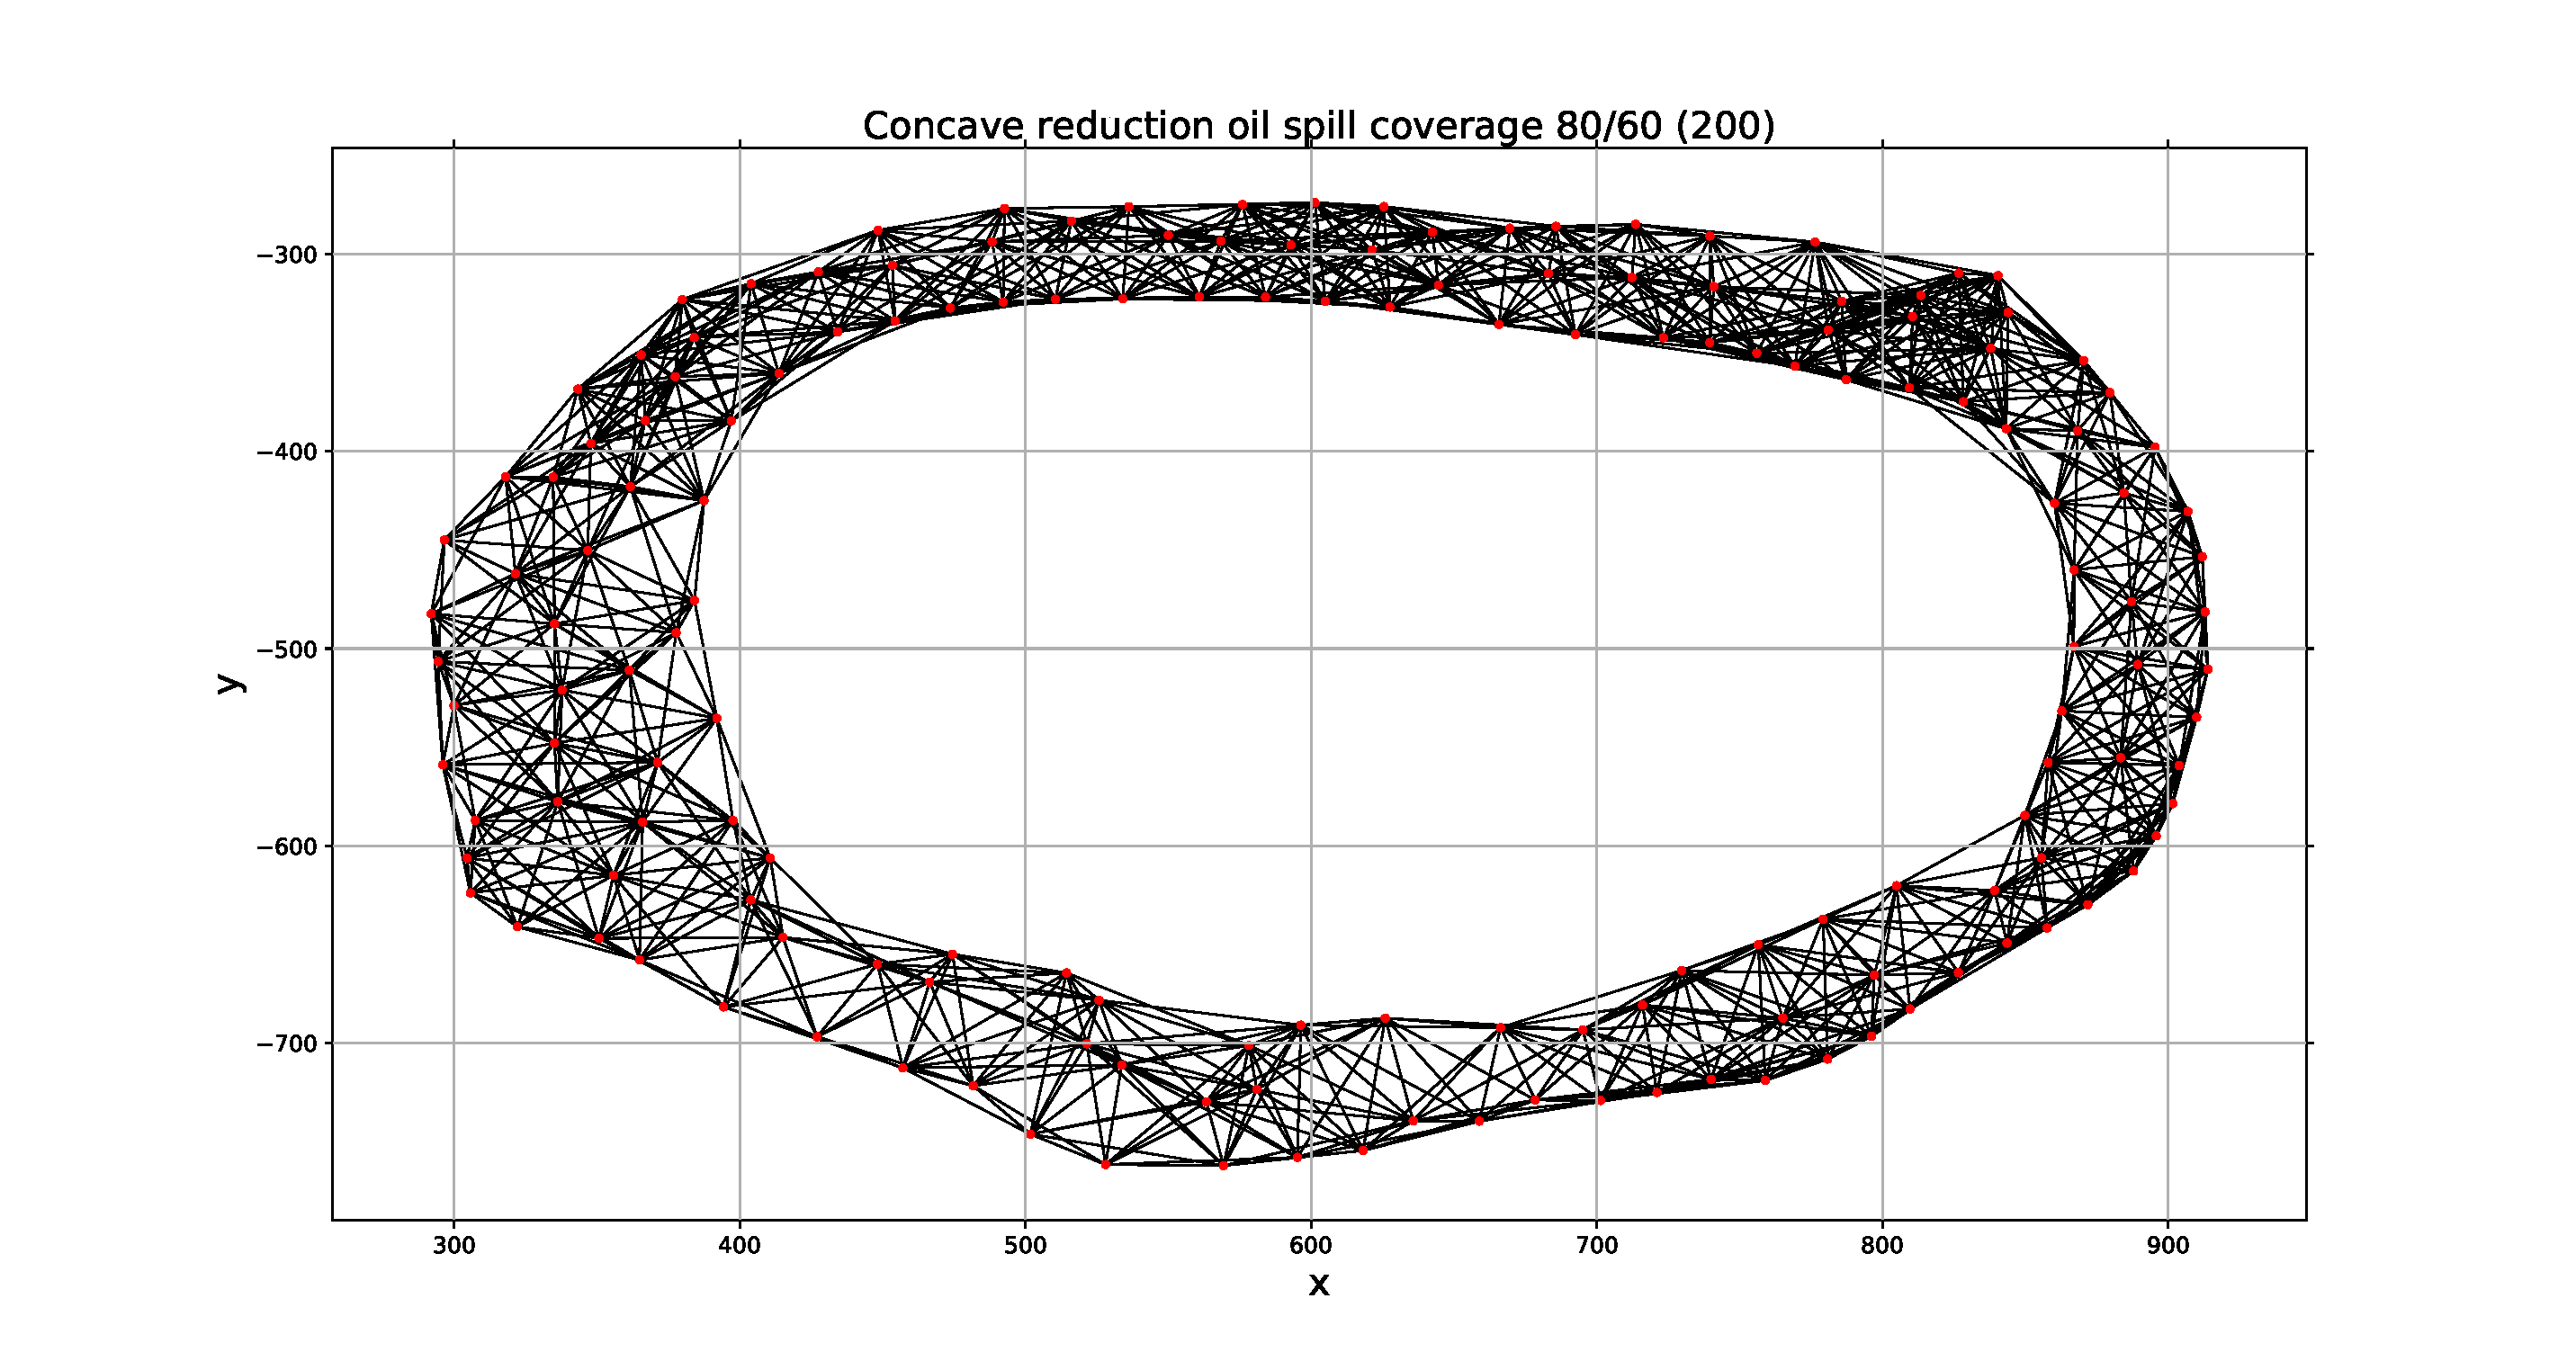
\includegraphics[width=6cm]{CHAPTER-7/figures/OilSpillConcave1}
    \label{concave:OilSpillConcave1}
}
\subfigure[Partial]{
    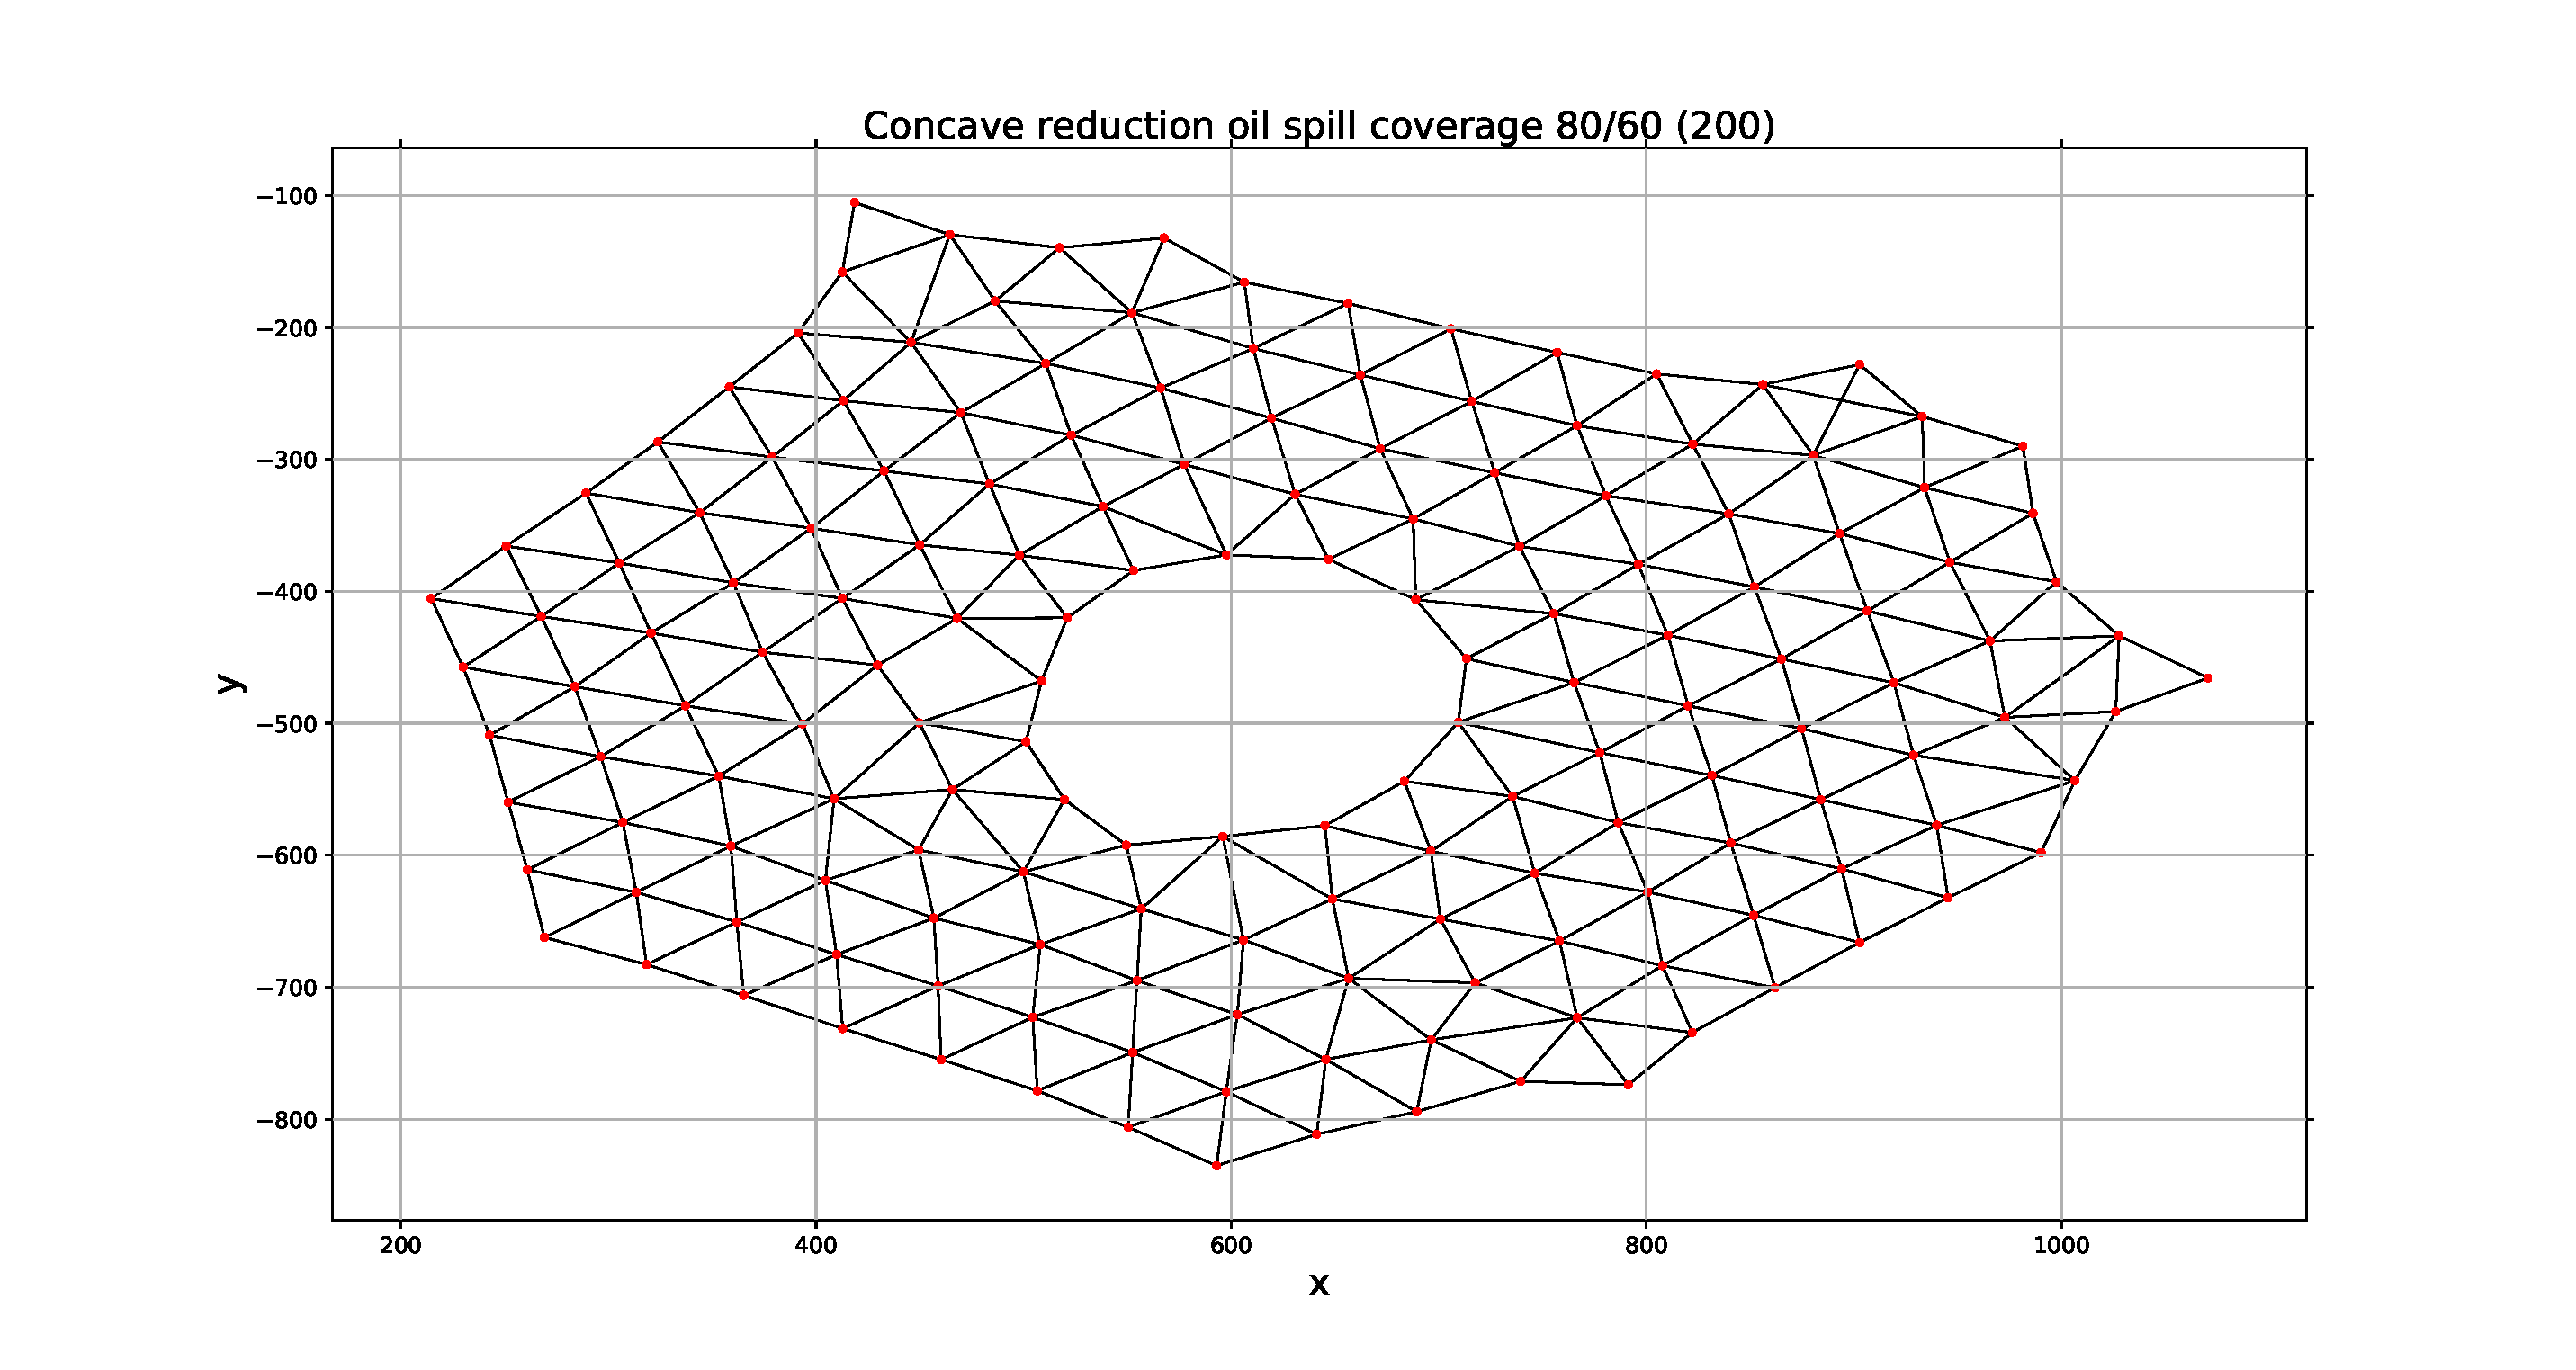
\includegraphics[width=6cm]{CHAPTER-7/figures/OilSpillConcave2}
    \label{fig:OilSpillConcave2}
}
\subfigure[End]{
    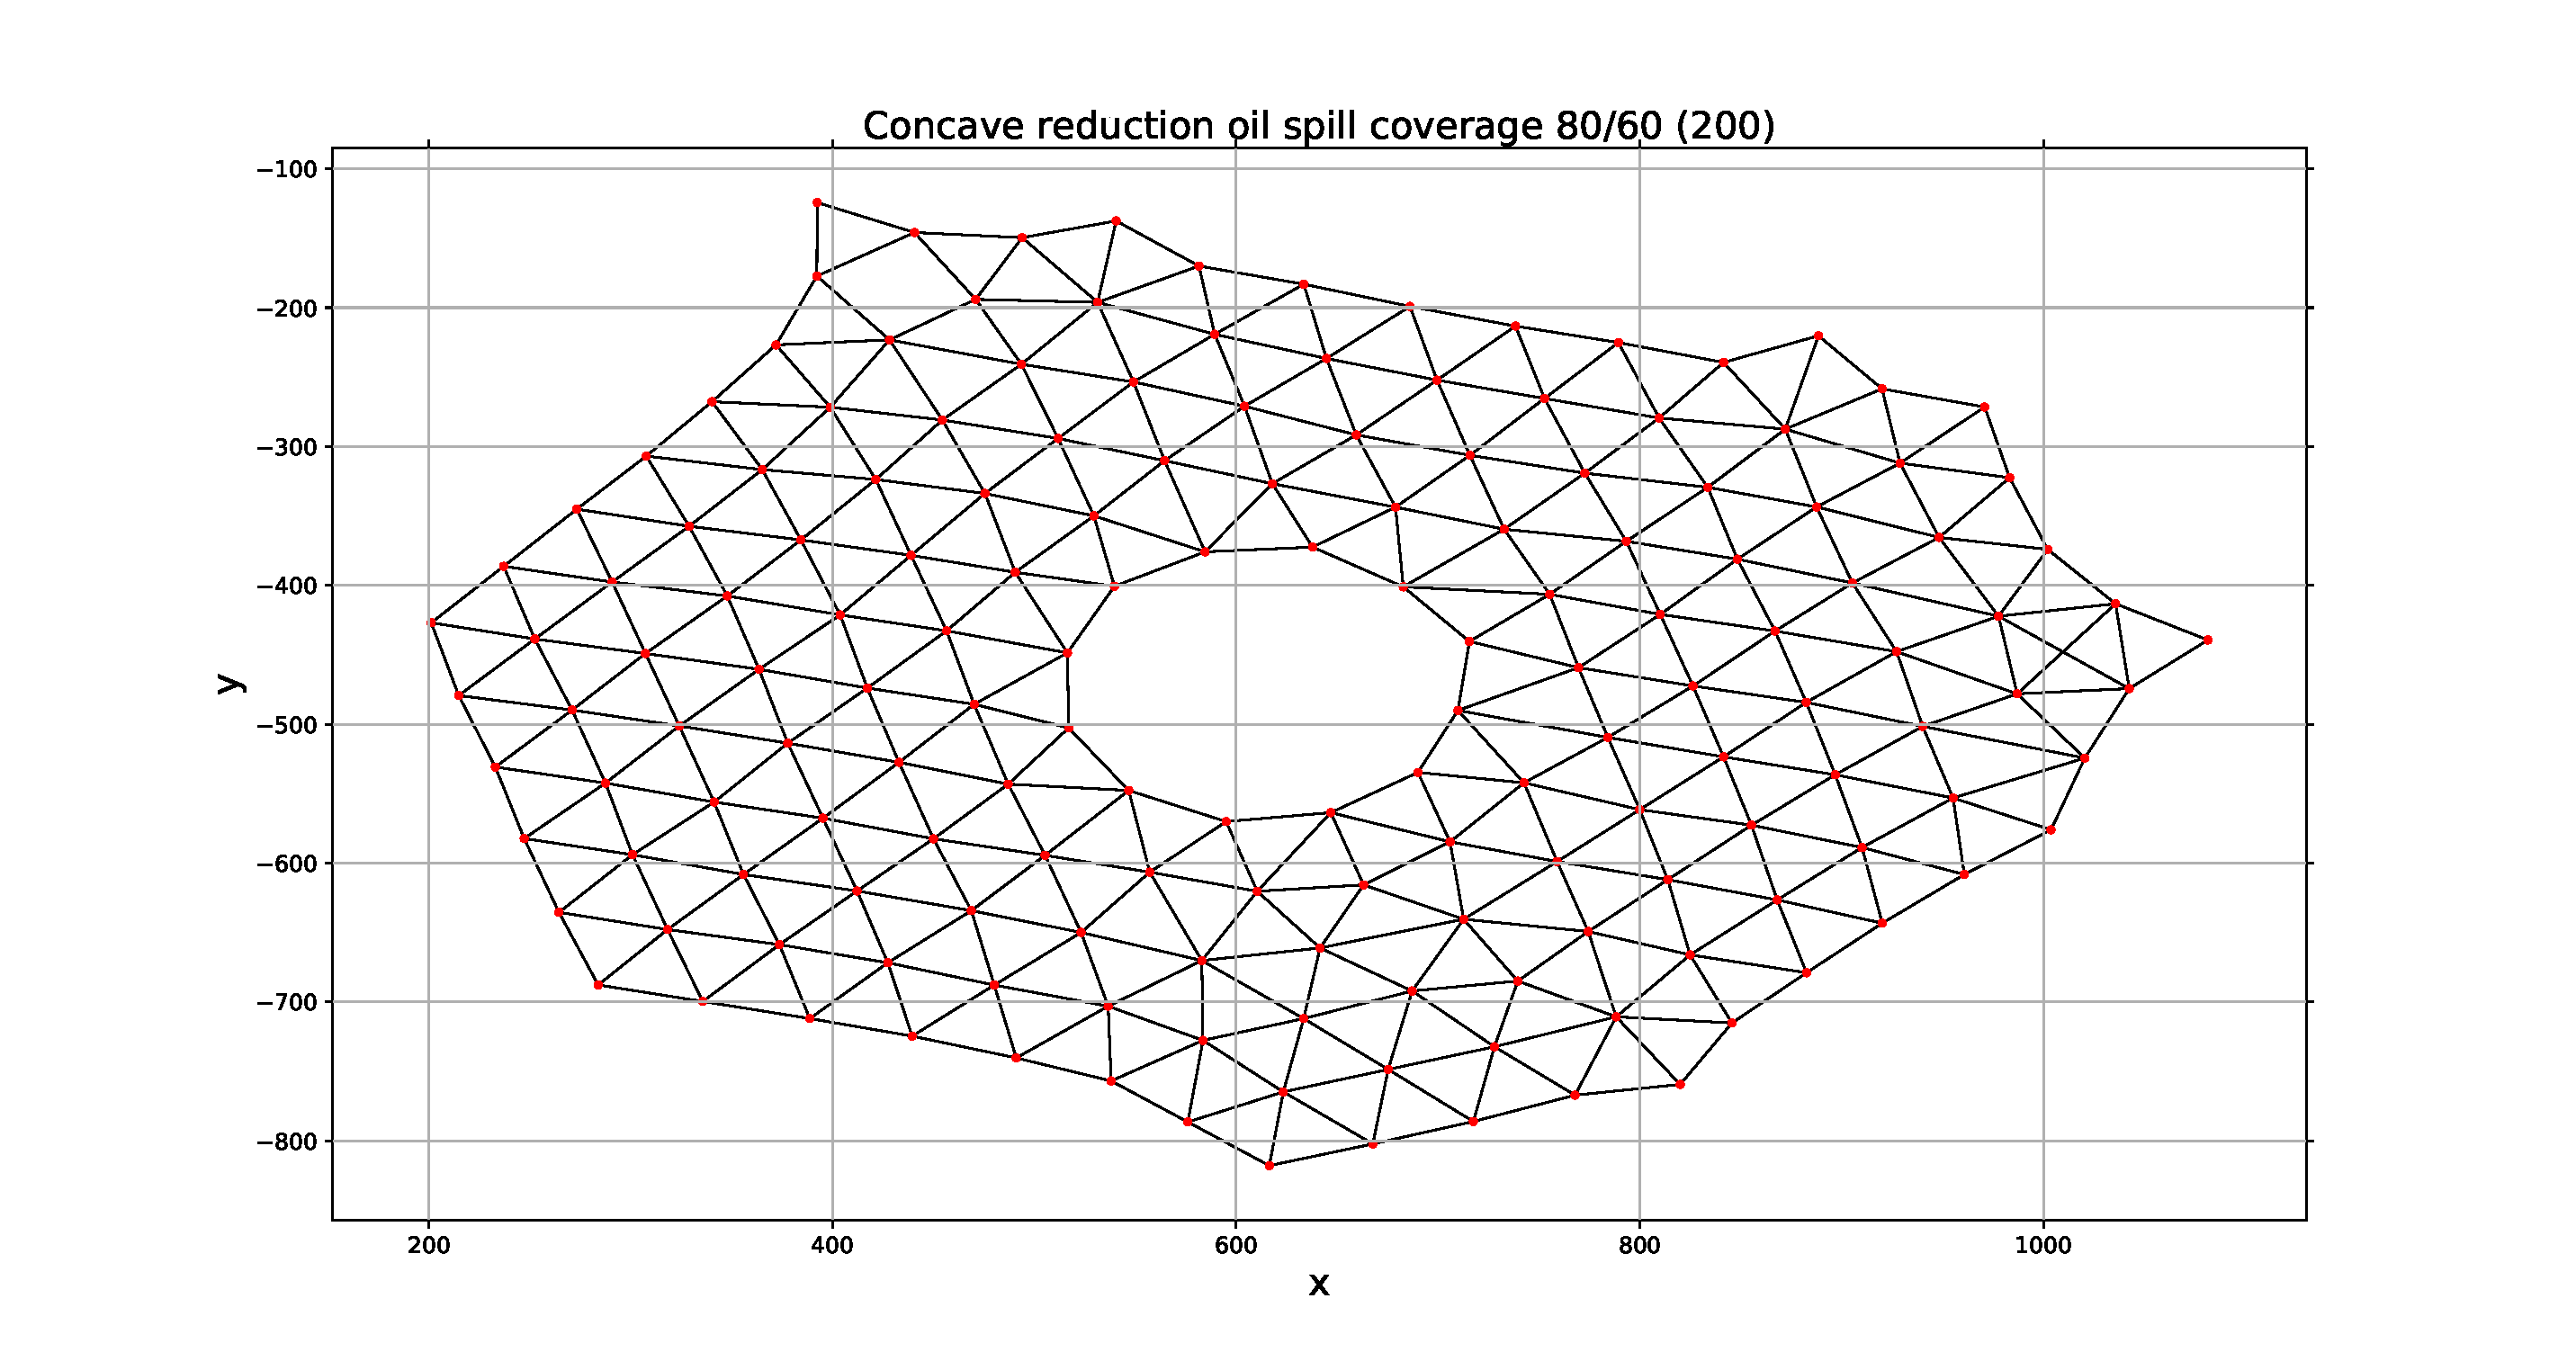
\includegraphics[width=6cm]{CHAPTER-7/figures/OilSpillConcave3}
    \label{fig:OilSpillConcave3}
}
\caption{Concave reduction spill containment}
\label{fig:OilSpillConcaveReduction}
\end{figure}

Figures \ref{concave:OilSpillPerimeter8060-DIST-1} and \ref{concave:OilSpillPerimeter8060-MAG-1} show the effect of the concave reduction on the swarm's agent distribution compared to the baseline for the oil spillage scenario. 

Figure~\ref{concave:OilSpillPerimeter8060-DIST-1} shows distance distribution of the swarm for both the baseline (grey/black) and the concave reduction (red). The baseline expands then settles at approximately 6 seconds. This is also the case for the the concave reduction swarm. The baseline swarm, following the initial expansion, remains relatively slow changing with respect to distance and magnitude. The concave reduction swarm is affected more significantly, at approximately 10 seconds into the simulation the swarm's internal void perimeter makes contact with the oil spillage (obstacle). This has the effect of disrupting the average distance and average \textit{inter-agent magnitudes}. This effect diminishes slightly at approximately 18 seconds where the swarm's \textit{concavity reduction vectors} cause the swarm to surround the spillage. The surrounding is followed by a few remaining changes caused by the agents at the spillage perimeter `snapping', the surrounding process is complete.
%BASELINE-CONCAVE-OIL-DIST.py
\begin{figure}[H]
\begin{center}
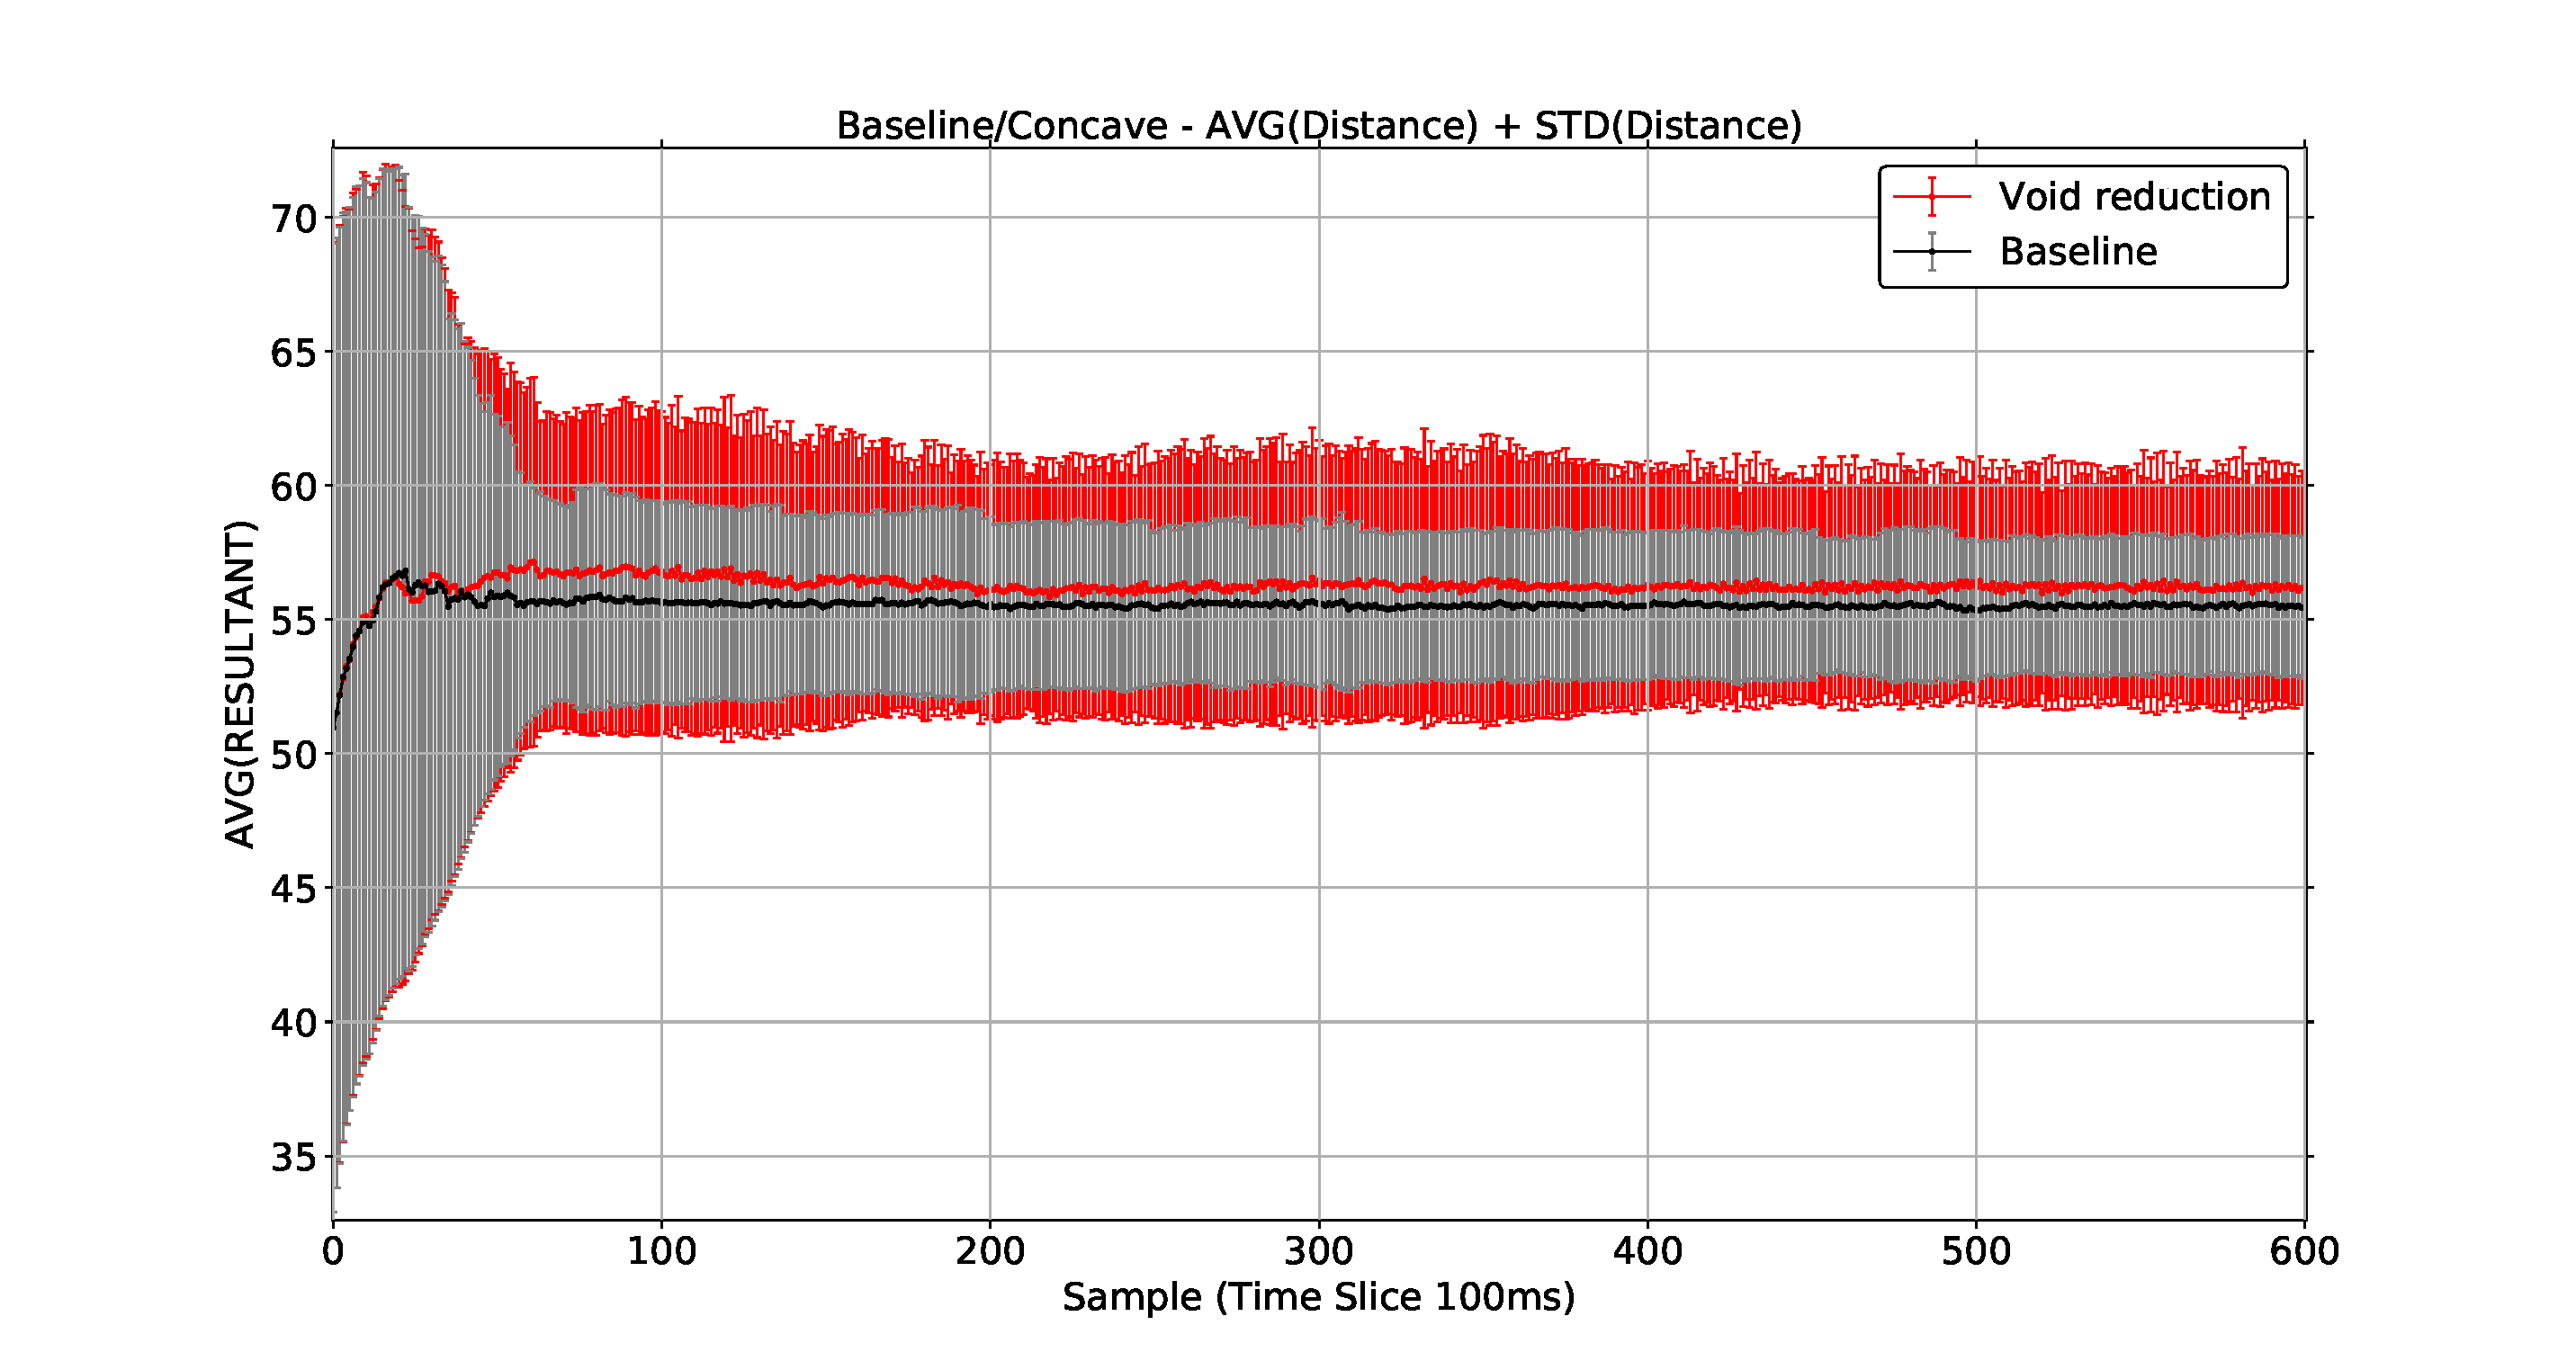
\includegraphics[width=14cm]{CHAPTER-7/figures/OilSpillPerimeter8060-DIST-1}
\end{center}
\caption{Oil spill containment distance\label{concave:OilSpillPerimeter8060-DIST-1}}
\end{figure}

Figure~\ref{concave:OilSpillPerimeter8060-MAG-1} shows the comparison of the \textit{inter-agent magnitudes} for the baseline and concave reduction swarms. The initial deployment of the swarm is so condensed that the average \textit{inter-agent magnitude} is negative which indicates a high level of expansion. Within 2 seconds the expansion has reached a point where the average magnitude is positive which indicates the swarm is cohesive and will therefore remain as a single entity and be capable of surrounding an object without breaking apart.
%BASELINE-CONCAVE-OIL-MAG.py
\begin{figure}[H]
\begin{center}
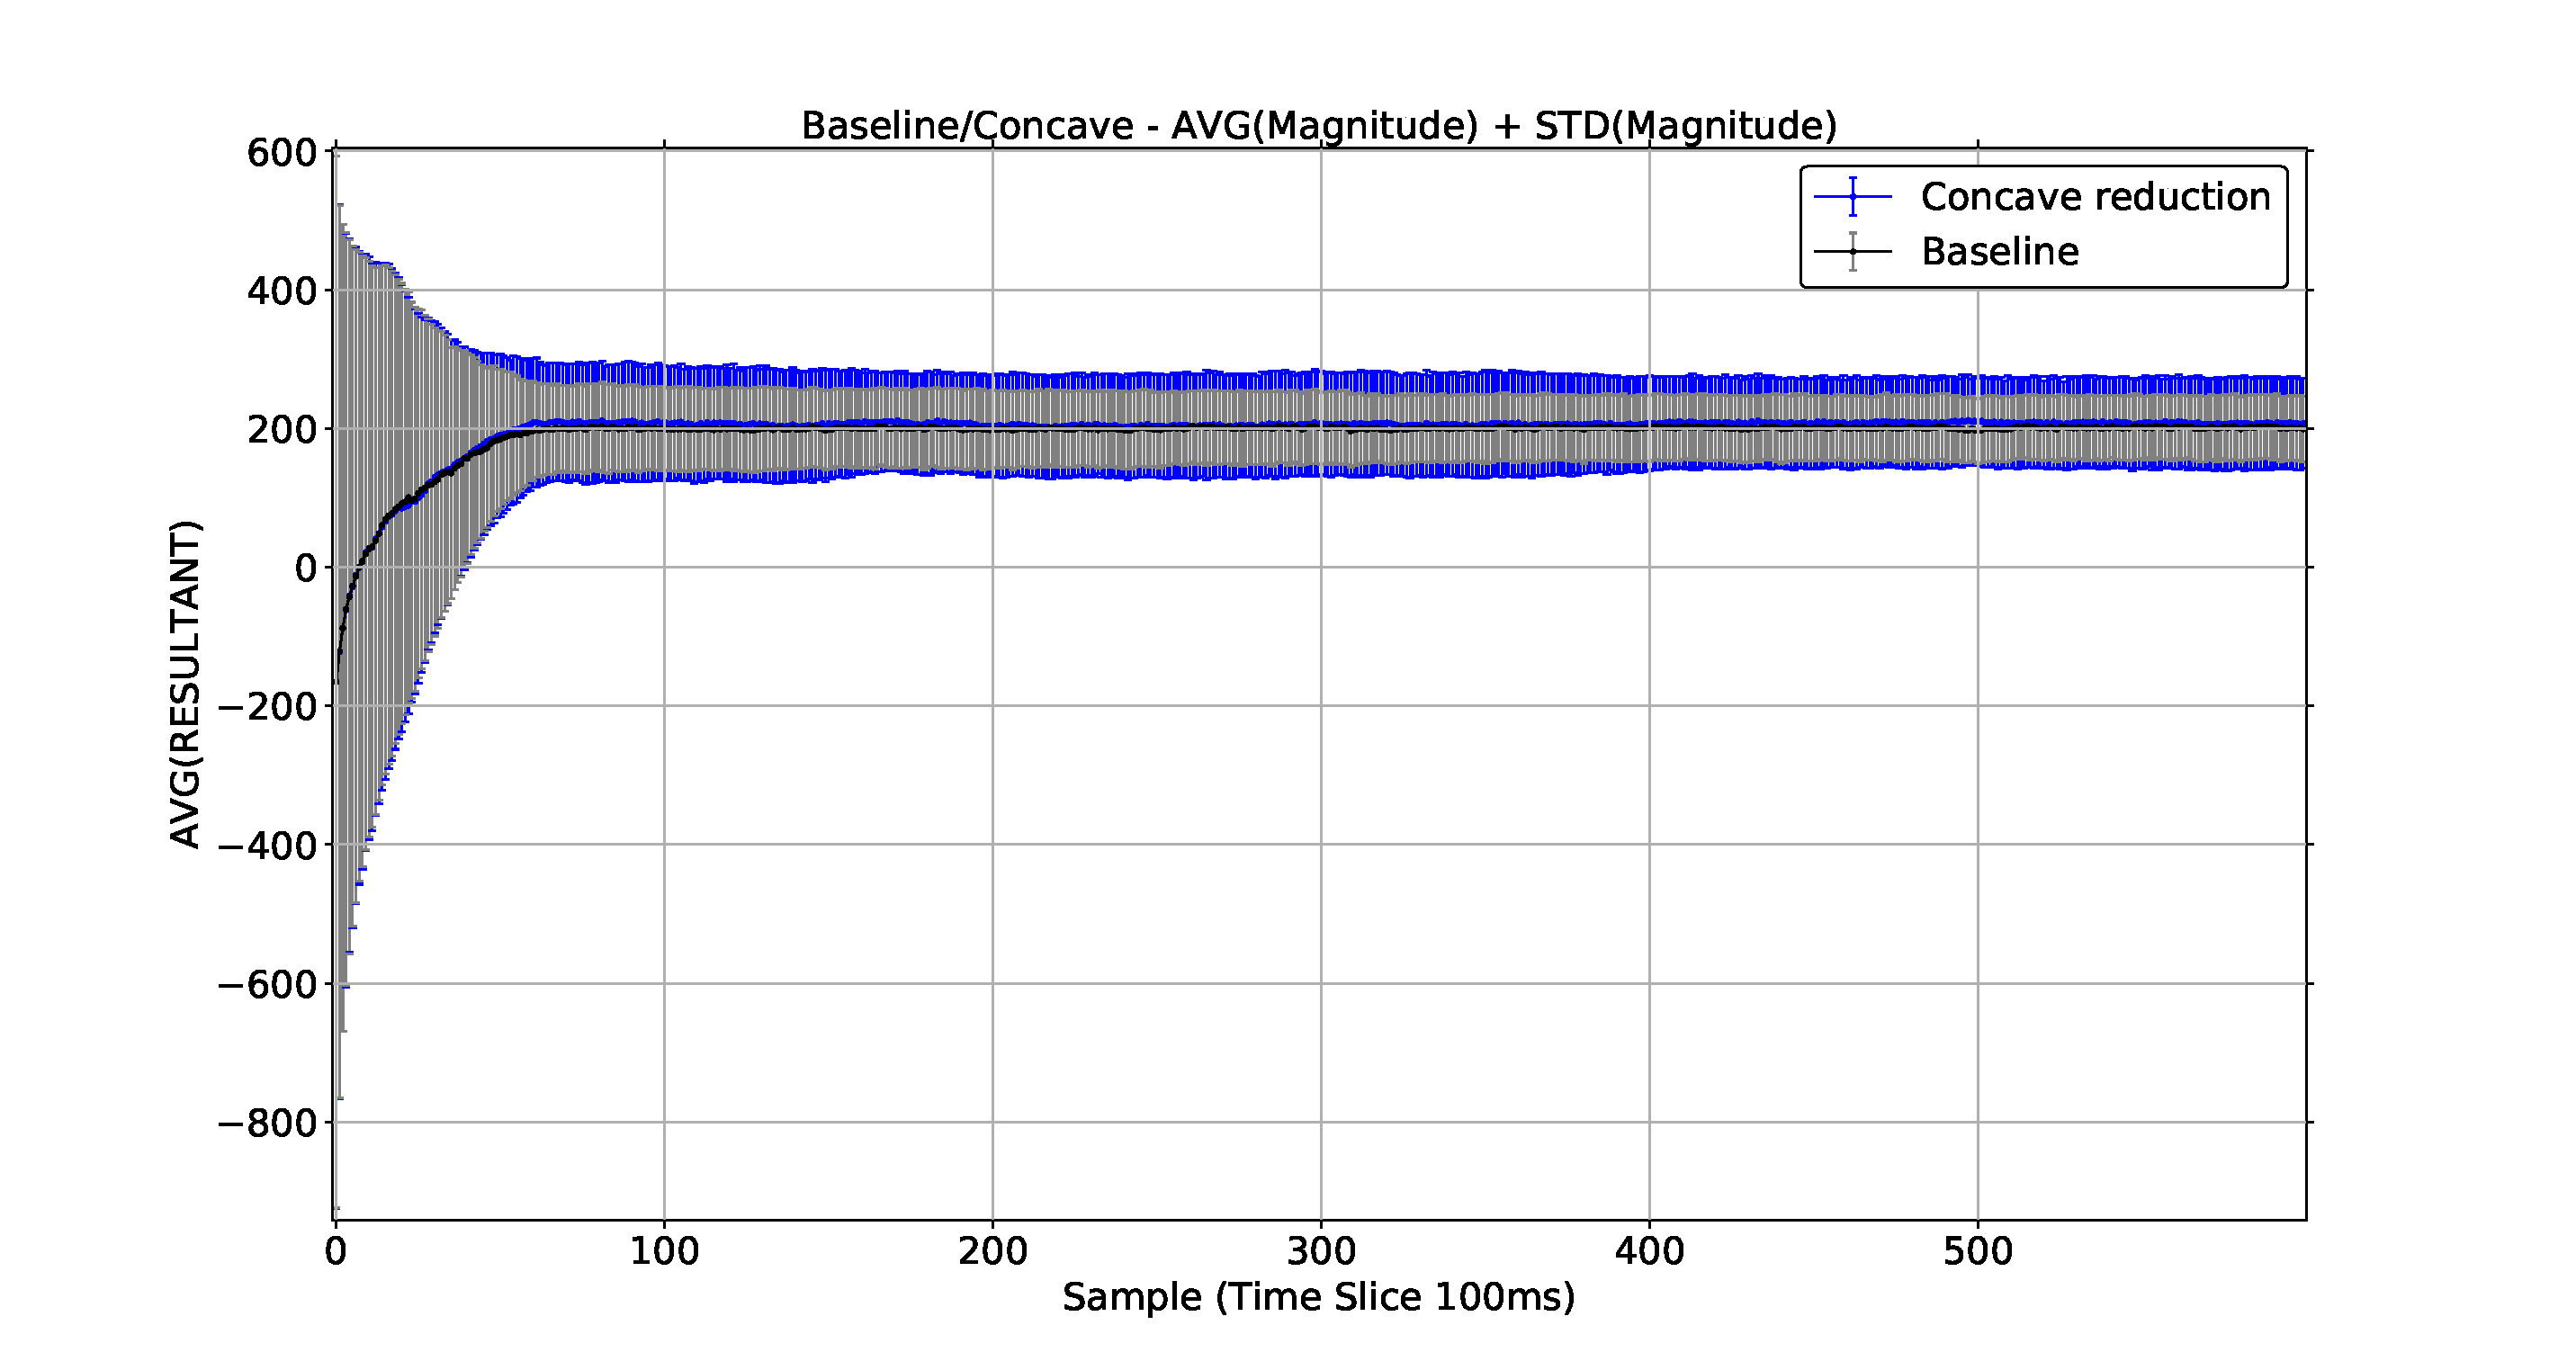
\includegraphics[width=14cm]{CHAPTER-7/figures/OilSpillPerimeter8060-MAG-1}
\end{center}
\caption{Oil spill containment magnitude\label{concave:OilSpillPerimeter8060-MAG-1}}
\end{figure}

When the swarm `shrinks' to surround the obstacle there is an erratic change in the number of perimeter agents. Figure~\ref{concave:OilSpillPerimeter8060-1} shows the number of perimeter agents identified over the duration of the simulation. The graph shows the baseline swarm perimeter size decreases steadily and then settles (The swarm has not enclosed the spillage). The perimeter count has settled but as shown in figures~\ref{concave:OilSpillPerimeter8060-DIST-1} and \ref{concave:OilSpillPerimeter8060-MAG-1} the agents are still moving (magnitude variance and magnitude \textgreater 0) but the movement does not effect the overall structure. 

In the case of the concave reduction swarm the perimeter size is erratic due to the snapping effect~(Figure~\ref{fig:InducedJitter}). When the swarm encounters the obstacle at approximately 10 seconds there is a change due to `snapping' as the agents `fold' around the obstacle. The perimeter size then continues to fall gradually as the void is percolated out of the system, the perimeter size then stabilises as the obstacle is fully surrounded.
%PERIMETEROILSPILL.py
\begin{figure}[H]
\begin{center}
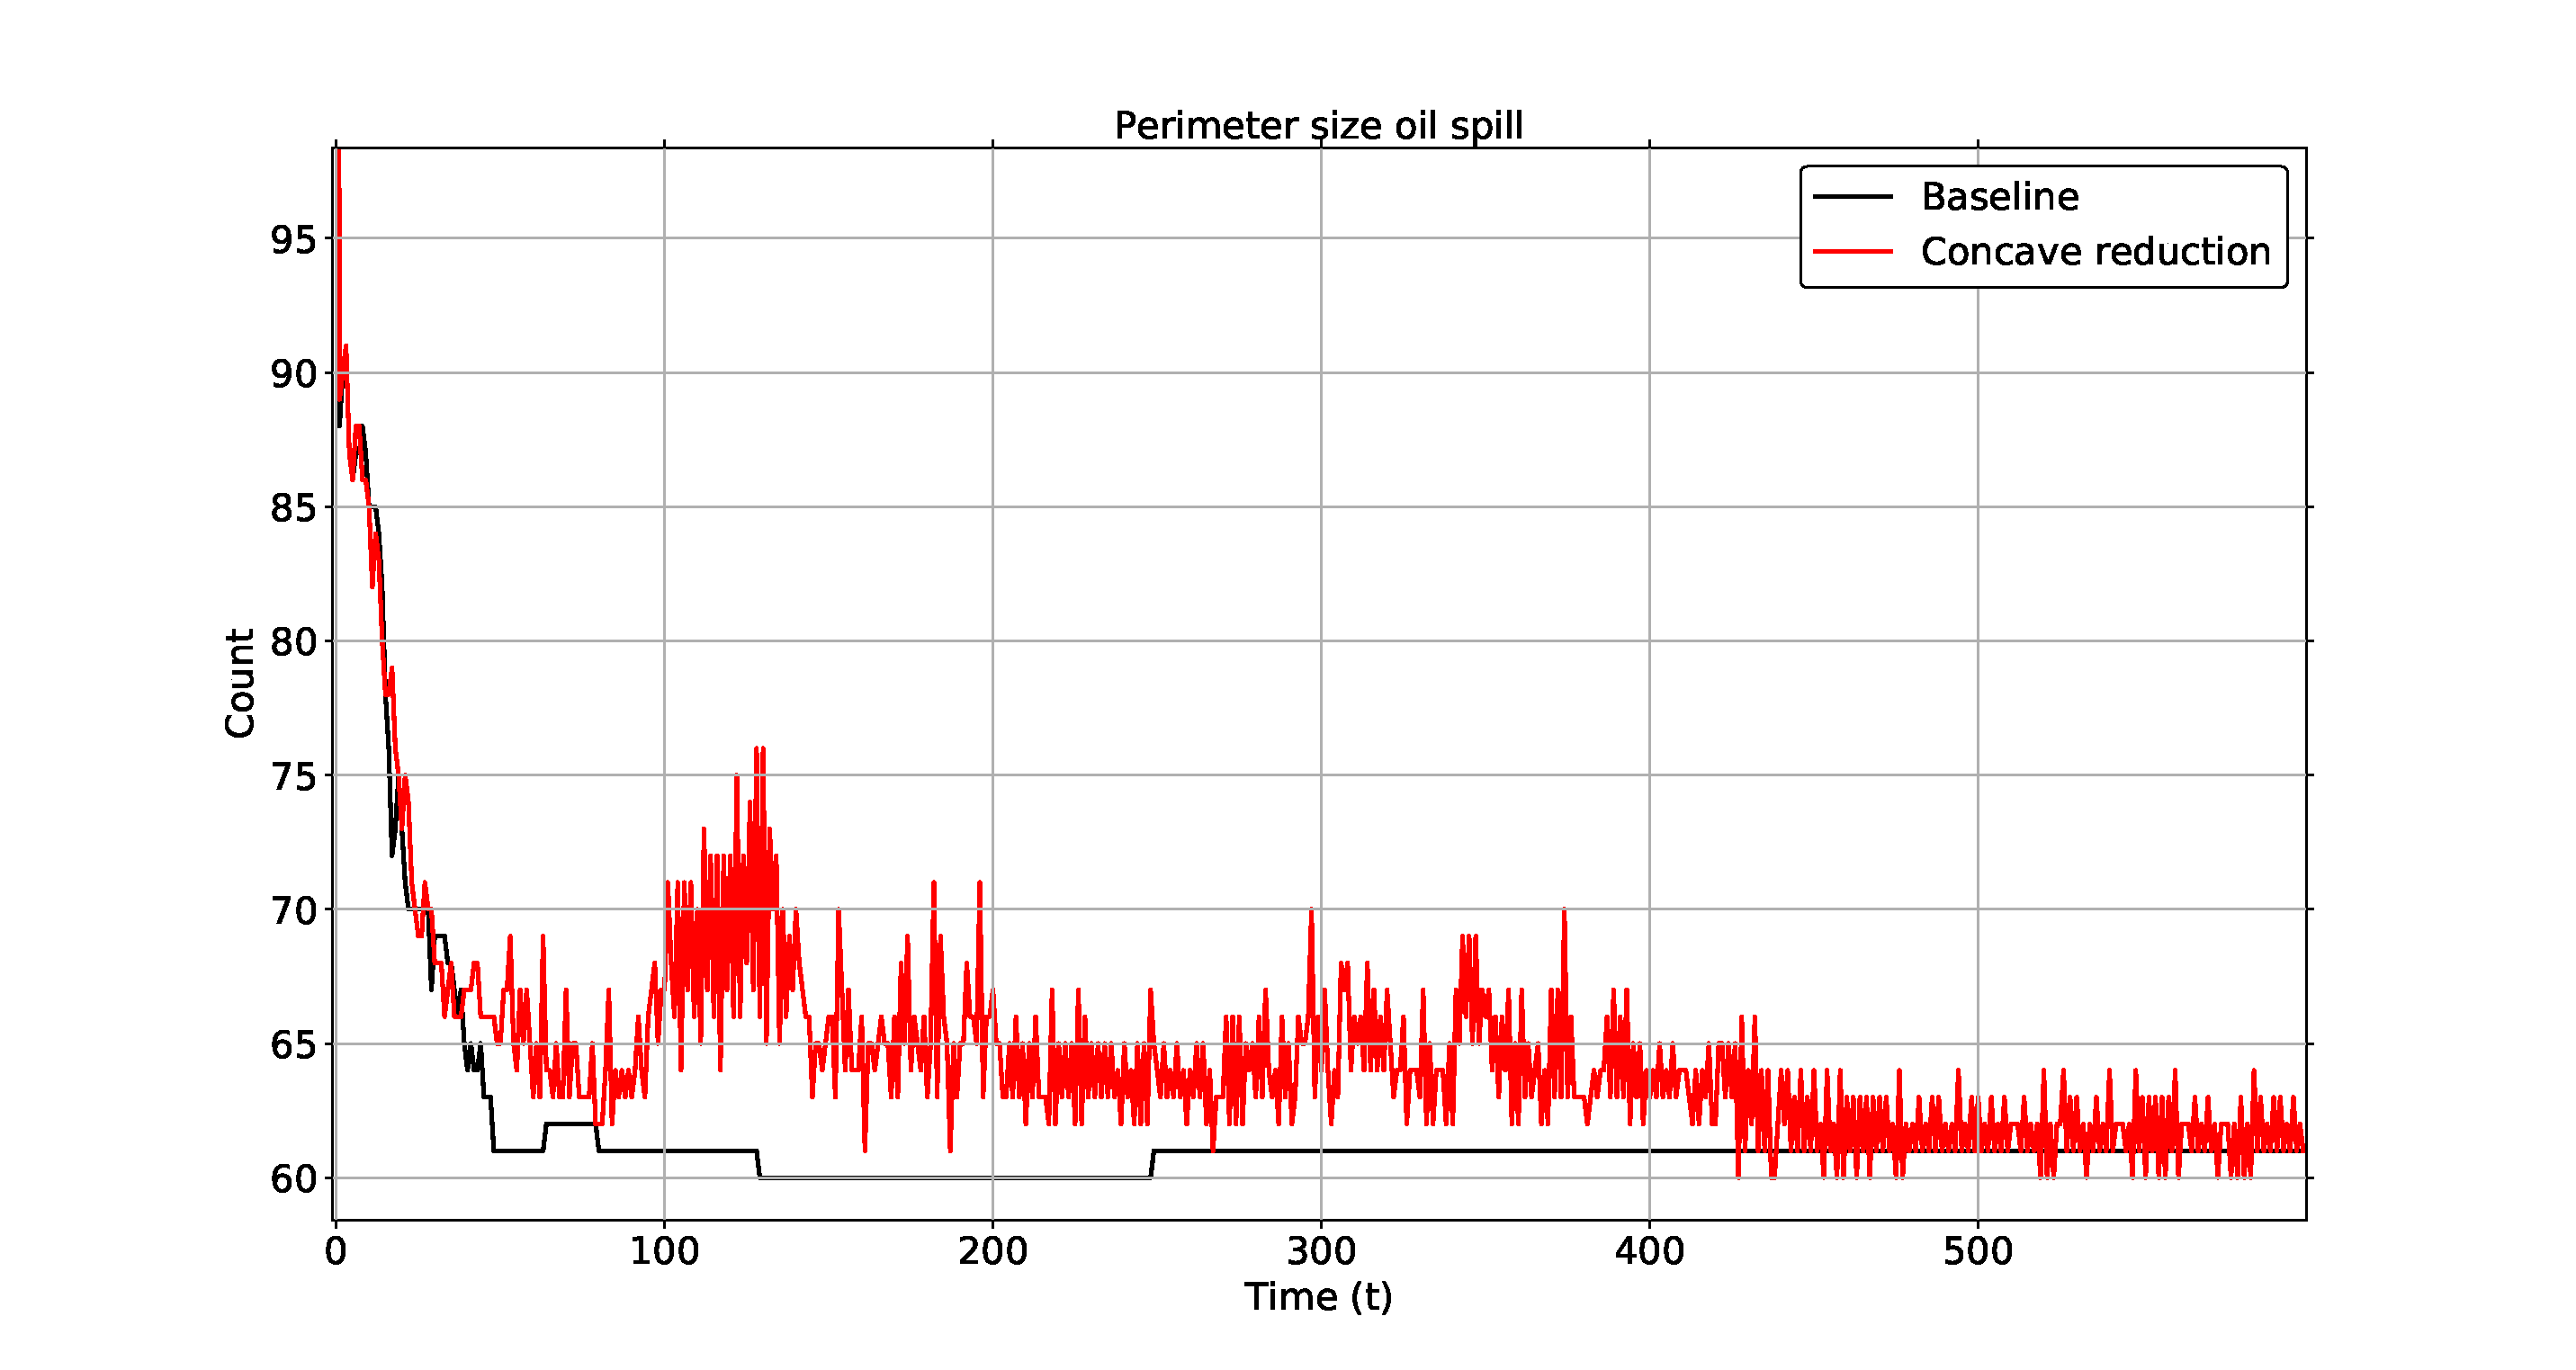
\includegraphics[width=14cm]{CHAPTER-7/figures/OilSpillPerimeter8060-1}
\end{center}
\caption{Swarm perimeter size comparison\label{concave:OilSpillPerimeter8060-1}}
\end{figure}

\section{Concave reduction for destination-based swarms}\label{concave:mobileSwarm1}
A goal based swarm that is travelling between two points can have its path disrupted by an obstacle. This event can cause a swarm to develop an anomaly in the form of a void~(Figure~\ref{concave:PerimeterObject2}) due to agents temporarily separating as the swarm passes the obstacle or the swarm may split entirely if the obstacle is very large~(Figure~\ref{concave:PerimeterObject1}). 

When the object is small the cohesion and repulsion fields may make the swarm naturally reform~(Figure~\ref{concave:PerimeterObject2}), however as the swarm progresses past the obstacle a void is created at the forward edge of the obstacle. If the purpose of the swarm is to deploy fertilizer over crops or carry out a reconnaissance task then the required full area coverage is not achieved. This failure to achieve total coverage reduces the effectiveness of employing a swarm to carry out tasks of this type.

\begin{figure}[H]
\centering
\subfigure[Swarm distortion via an object creating a void]{
	 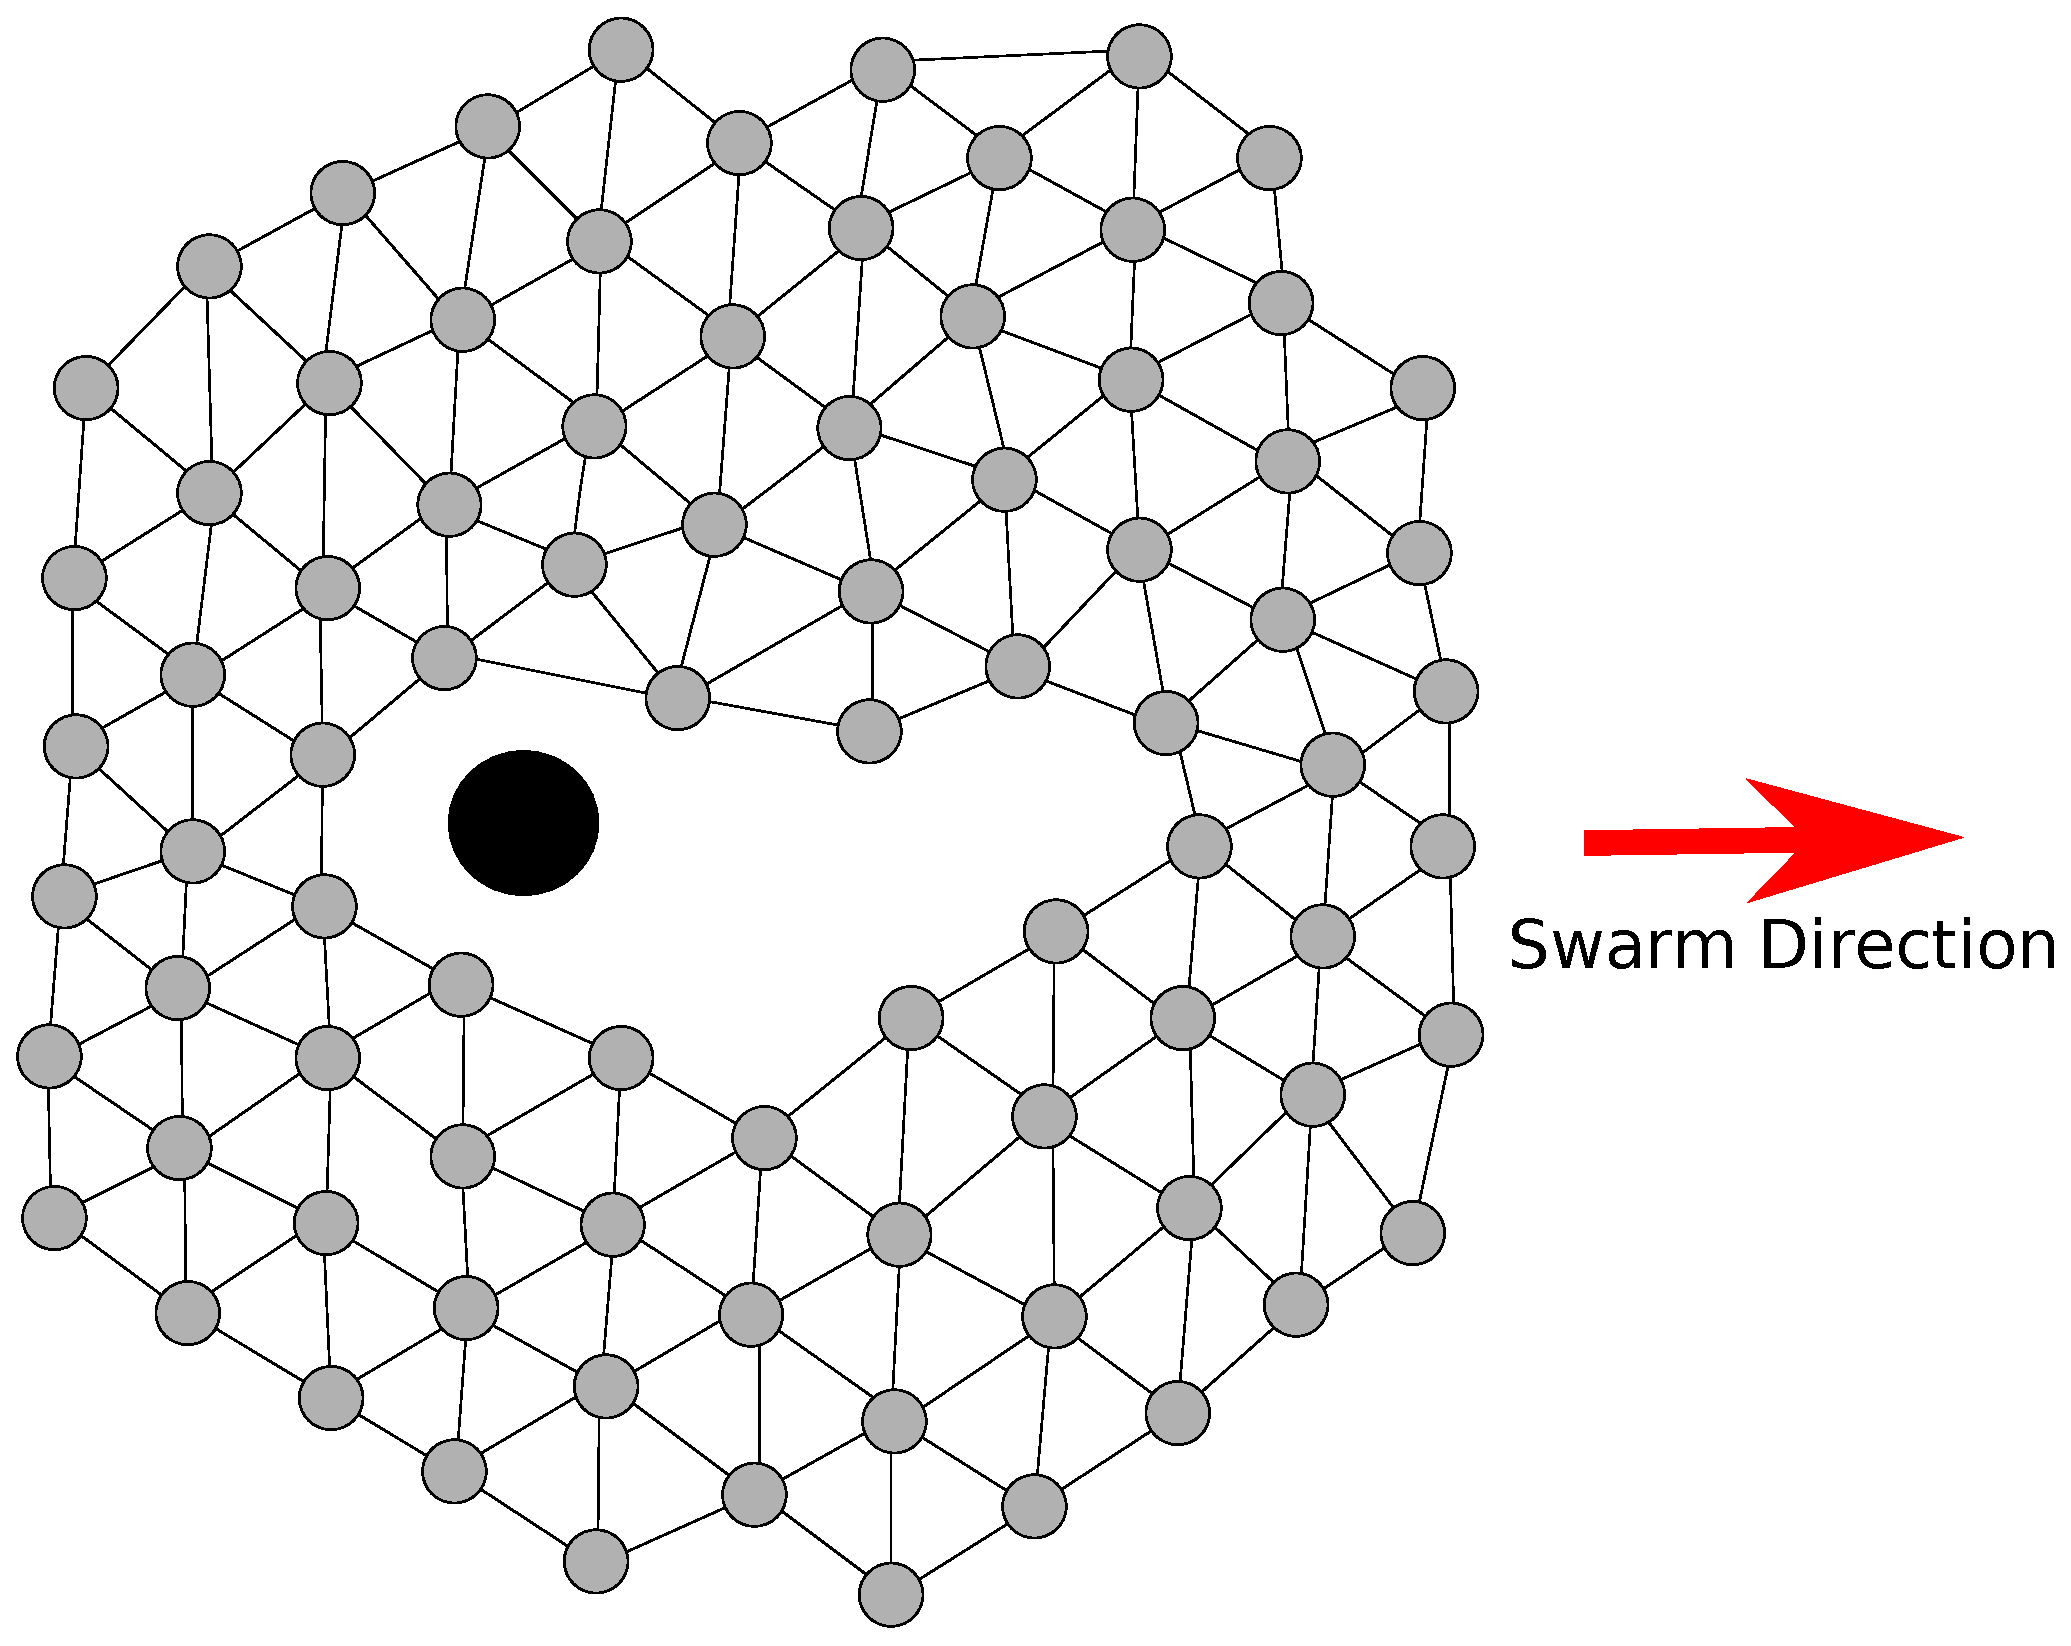
\includegraphics[width=6.2cm]{CHAPTER-7/figures/PerimeterObject2}
    \label{concave:PerimeterObject2}
}
\subfigure[Swarm distortion via a large object]{
    \includegraphics[width=5cm]{CHAPTER-7/figures/PerimeterObject1}
    \label{concave:PerimeterObject1}
}
\caption{Swarm perimeters and voids}
\label{fig:SwarmObjectVoids}
\end{figure}
 
Concave reduction has been shown to remove voids in static swarms in~section~\ref{sec:ApplicationConcavePerimeters}. Concave reduction can also be applied to a goal-based swarm to control coverage when passing small object: `small' means the maximum radius of the obstacle is of the order of the size of the neighbour field of an agent or less. When concave reduction is applied to the swarm it will surround the obstacle. Surrounding the obstacle creates a greater degree of coverage and increases the effectiveness of the swarm.

Taking the baseline swarm from chapter~\ref{chapter:coordination} the swarm environment can be modified to include an obstacle in the path of the swarm. Table~\ref{tab:SwarmCoverageParameters} shows the weightings and field effects for the baseline and concave reduction parameters for the experiment to demonstrate the concave reduction coverage improvement. Figure~\ref{voids:ObstacleTest1} shows the swarm and object setup within the simulator for the experiment.

\begin{table}[H]
\begin{center}
\begin{tabular}{| p{2.3cm} | p{2.3cm} | p{5cm} |}
\hline
\bf Weight \bf component & \bf Baseline \bf swarm & \bf Description \\ \hline
Sample rate & 100 & ms - Unit sampling interval\\  \hline
$k_{cr}$ & 100 & weight adjuster for concavity vector\\  \hline
$k_o$ & 100 & weight adjuster for obstacle field\\  \hline
$k_c$ & 5 & weight adjuster for cohesion field\\  \hline
$k_r$ & 15 & weight adjuster for repulsion  field\\  \hline
$k_d$ & 35 & weight adjuster for destination vector\\  \hline
Repulsion Boundary & 45 & units\\  \hline
Neighbour Distance & 60 & units\\  \hline
Obstacle size & 60 & units\\  \hline
Speed & 20 & units/s\\  \hline
\end{tabular}\caption{Swarm coverage parameters}\label{tab:SwarmCoverageParameters}
\end{center}
\end{table}

\begin{figure}[H]
\begin{center}
\includegraphics[width=10cm]{CHAPTER-7/figures/ObstacleTest}
\end{center}
\caption{Initial configuration\label{voids:ObstacleTest1}}
\end{figure}

The experiment was run for 60 seconds to determine how the swarm is affected by the obstacle. The experiment is executed twice once with and once without concave reduction enabled. For figures~\ref{voids:ObstacleTest2} and \ref{voids:ObstacleTest3} the blue lines are generated by plotting the position of each agent as they progress towards the goal. Figure~\ref{voids:ObstacleTest2} is a path trace of the swarm as it propagates around the obstacle without concave reduction. The agents are repelled by the obstacle and the leading edge `flows' around the perimeter. Due to the compression caused by the agents passing around the obstacles an expansion is experienced at the trailing side and the agents are `pushed' such that the swarm reforms. However the time it takes for the compression to be removed causes the swarm to create a void at the forward side of the obstacle.  

\begin{figure}[H]
\begin{center}
\includegraphics[width=15cm]{CHAPTER-7/figures/SWARMCOVER456060BASELINE}
\end{center}
\caption{Swarm without concave reduction (repulsion field 60 units for obstacle)\label{voids:ObstacleTest2}}
\end{figure}

Figure~\ref{voids:ObstacleTest3} shows the path trace for the same environment settings with concave reduction enabled. In a similar way to the baseline experiment the leading edge agents approach the obstacle and through the repulsion effect of the obstacle the agents travel around the outer edge. Once the agents have passed the mid point of the obstacle the swarm splits in a similar way to the original experiment. The void is created in a similar way but when the split segments converge a change occurs. The meeting edges create a concave edge and the \textit{concavity reduction vectors} affect the agents by `pulling' the `edges' together. This effect propagates back along the edges until the concave perimeter is reduced back to the obstacles forward edge. This effect slows the progress of the swarm's internal movement but closes the void. As the swarm progresses towards the destination the back portion of the swarm moves around the obstacle and swarm continues onto the destination.

\begin{figure}[H]
\begin{center}
\includegraphics[width=12cm]{CHAPTER-7/figures/SWARMCOVER456060CONCAVE}
\end{center}
\caption{Swarm with concave reduction (repulsion field 60 units for obstacle)\label{voids:ObstacleTest3}}
\end{figure}

\section{Conclusion}\label{voids:Conclusion}
This chapter has demonstrated the concept of controlling a swarm's structure through the identification of perimeter anomalies in the form of concave edges. The identification of the anomalies is achieved locally by an individual agent without needing any communications infrastructure. The technique works with arbitrary sized swarms demonstrated here experimentally with a swarm of 200 agents.

Concave reduction is shown to work with static swarms such that a swarm can stablise to a more regular shape. It is possible for a swarm to develop where no concave reduction will be in operation which would allow the swarm to refer back to a baseline condition. Figure~\ref{voids:IdealSwarm} shows an ideal swarm shape that would result in no concave reduction based movement. 

\begin{figure}[H]
\begin{center}
\includegraphics[width=6cm]{CHAPTER-7/figures/IdealSwarm}
\end{center}
\caption{Swarm structure with no concave reduction\label{voids:IdealSwarm}}
\end{figure}

The chapter demonstrates by experiment that by altering the vector calculations for an agent based upon a set of stimuli it is possible to improve the coverage of an area and also create a `compression' effect that can increase the application landscape for swarming technologies that incorporate concave reduction.
